\documentclass{beamer}
\usetheme{Madrid}
\usepackage{graphicx}
\usepackage{amsmath}
\usepackage{hyperref}
\usepackage{graphicx}
\usepackage{amsmath}
\usepackage{amsfonts}
\usepackage{tikz}
\usetikzlibrary{shapes, arrows, positioning, calc}
\usepackage{multirow}
\usepackage{subcaption}

\title[NoMaD]{NoMaD: \textbf{N}avigati\textbf{o}n with Goal-\textbf{Ma}sked \textbf{D}iffusion}
\author{Abhishek,Namashivayaa, \\ Sehaj, Shobhnik}
\institute{IISc Bengaluru \newline BTech. Mathematics and Computing}
\date{April 2025}

\begin{document}

\begin{frame}
\titlepage
\end{frame}

\begin{frame}{Motivation and Goal}
    \textbf{Robotic navigation in unfamiliar environments requires:}
    \begin{itemize}
        \item Task-oriented navigation — reaching specified goals
        \item Task-agnostic exploration — discovering and mapping new areas
    \end{itemize}
    \pause
    \begin{block}{The Challenge}
        These two objectives are typically handled by \textit{separate systems}.\\[1ex]
        Exploration can be decomposed into:
        \begin{itemize}
            \item \textbf{Local Exploration:} Learning short-horizon control policies for diverse actions
            \item \textbf{Global Planning:} Using those policies to achieve long-horizon, goal-directed behavior
        \end{itemize}
    \end{block}
    \pause
    \begin{block}{Key Question}
        Can a \textit{single model} unify both tasks — exploration and navigation?
    \end{block}~
    \end{frame}
    \begin{frame}{What is NoMaD?}
        \textbf{NoMaD} is a transformer-based diffusion policy designed for long-horizon, memory-efficient navigation.\\[0.5em]
        It supports both:
        \begin{itemize}
            \item \textbf{Goal-conditioned navigation} — moving towards a specified visual goal
            \item \textbf{Open-ended exploration} — learning diverse behaviors without explicit goals
        \end{itemize}
        \pause
        \bigskip
        \texttt{NoMaD = \{EfficientNet + Vision Transformer\} $\leftarrow$ \textbf{ViNT} \\+ Diffusion Policies}
        \pause
        \bigskip
        \begin{block}{}
            It combines a transformer backbone to encode the high-dimensional visual stream, with diffusion models that predict a sequence of future actions in a generative manner.
        \end{block}
        \end{frame}

\begin{frame}{Overview of NoMaD Architecture}
    \begin{block}{Visual Goal-Conditioned Navigation}
        Backbone: ViNT (Visual Navigation Transformer)\\
        How does ViNT work?
        \begin{itemize}
            \item Recieves: A sequence of past and current observations $o_t$=$o_{t-P:t}$
            \item \textbf{Visual Encoder:} Each observation is processed using an EfficientNet-B0 encoder to extract feature embeddings.
        \end{itemize}
        \pause
        \texttt{EfficientNet?}
        \begin{itemize}
            \item A new method of Scaling CNNs to improve accuracy and efficiency
            \item It uses a \textbf{compound scaling} to uniformly scale all dimensions of depth, width, and resolution.
        \end{itemize}
    \end{block}
\end{frame}
\begin{frame}
    \begin{figure}
        \centering
        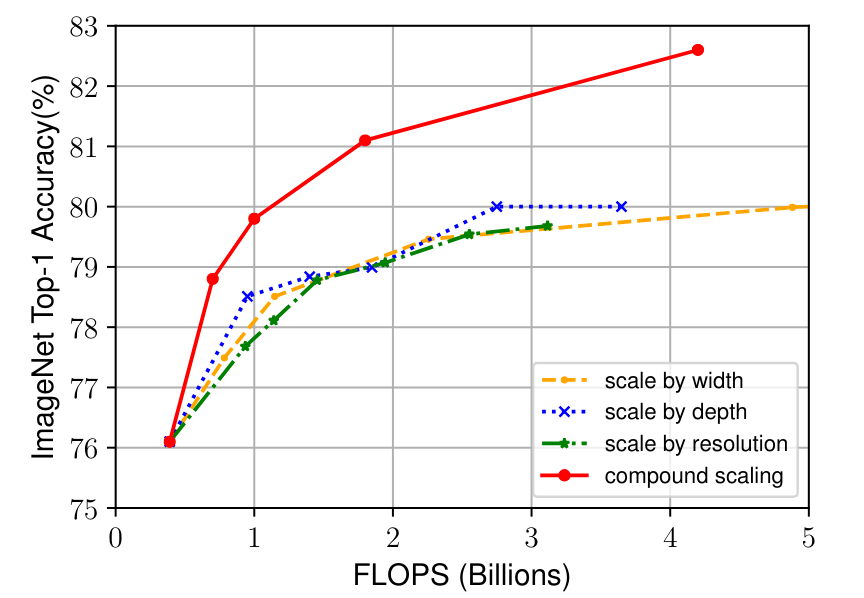
\includegraphics[width=0.8\linewidth]{effnet_scaling.png}
        \caption{Compound Scaling}
        \label{fig:efficientnet}
    \end{figure}
\end{frame}
\begin{frame}{EfficientNet}
    \begin{block}{}
        Use Network Architecture Search (NAS) to find the best baseline network (EfficientNet-B0)\\
        \bigskip
        \textbf{Optimization Objective:}
    \[
    \text{ACC}(m) \times \left[\frac{\text{FLOPS}(m)}{T}\right]^w
    \]
    \begin{itemize}
        \item $\text{ACC}(m)$: accuracy of model $m$
        \item $\text{FLOPS}(m)$: floating point operations
        \item $T$: target FLOPS
        \item $w = -0.07$: controls trade-off between accuracy and FLOPS
    \end{itemize}
    \end{block}
\end{frame}
\begin{frame}{EfficientNet Scaling}
    \begin{block}{\textbf{Compound Scaling}}
        EfficientNet introduces a principled way to scale up CNNs using a single compound coefficient $\phi$.
        \begin{itemize}
            \item Simultaneously scales:
            \begin{itemize}
                \item Network depth $d$
                \item Width $w$
                \item Input resolution $r$
            \end{itemize}
            \item Scaling formulas:
            \[
            d = \alpha^\phi, \quad w = \beta^\phi, \quad r = \gamma^\phi
            \]
            \item Constants $\alpha$, $\beta$, and $\gamma$ are determined via grid search.
        \end{itemize}
        \vspace{0.3em}
        \textbf{Subject to constraint:}
        \[
        \alpha \cdot \beta^2 \cdot \gamma^2 \approx 2
        \]
        Ensures that the model scales within a fixed computational budget.
    \end{block}
\end{frame}
\begin{frame}
    \begin{figure}
        \centering
        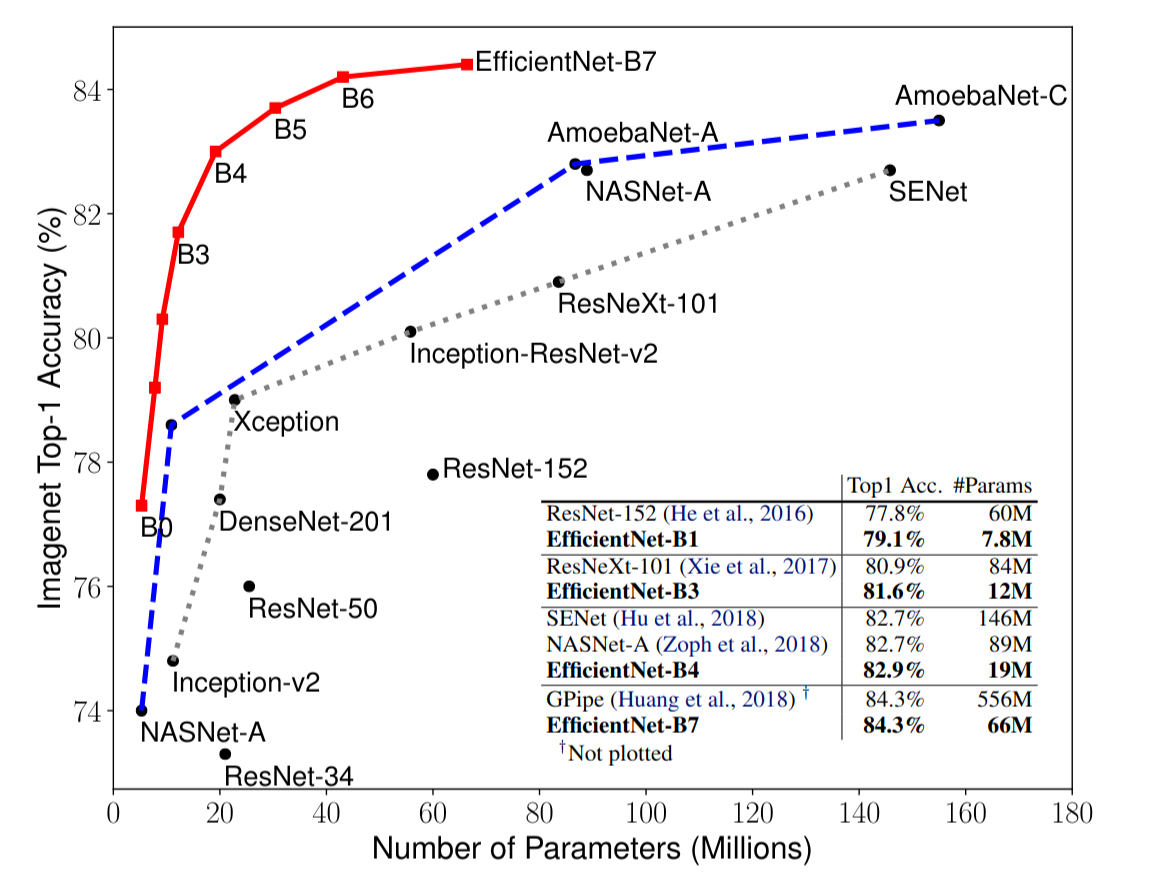
\includegraphics[width=0.8\linewidth]{effnet_imagenet.png}
        \caption{Accuracy on imagenet}
        \label{fig:efficientnet}
    \end{figure}
\end{frame}


\begin{frame}{Overview of NoMaD Architecture}
    \begin{block}{Visual Goal-Conditioned Navigation}
        Backbone: ViNT (Visual Navigation Transformer)\\
        How does ViNT work?
        \begin{itemize}
            \item Recieves: A sequence of past and current observations $o_t$=$o_{t-P:t}$
            \item \textbf{Visual Encoder:} Each observation is processed using an EfficientNet-B0 encoder to extract feature embeddings.
            \pause
            \item \textbf{Goal Fusion:} The current and goal images are combined using a goal-fusion encoder.
            \item \textbf{Transformer Attention:} These fused features (tokens) are passed through a Transformer model to generate a context vector $c_t$.
            \item \textbf{Predictions:} The context vector is used to predict:\\
            -A distribution over future actions: $a_t = f_a(c_t)$\\
            -An estimate of temporal distance to the goal: $d(o_t, o_g) = f_d(c_t)$
        \end{itemize}
    \end{block}
\end{frame}
\begin{frame}{Extending to Long-Horizon Planning with Topological Memory}
    \alert{However, ViNT is inherently goal-conditioned—it cannot operate in the absence
    of a goal image, limiting its ability to explore autonomously.}
    \pause
    \begin{block}{Solution}
        To enable open-ended exploration, NoMaD incorporates a Topological Memory $\mathcal{M}$:
        \begin{enumerate}
            \item Nodes represent previously encountered visual observations.
            \item Edges represent traversable paths, established using ViNT's predicted distances.
        \end{enumerate}
        This enables:
        \begin{itemize}
            \item \textbf{Subgoal Planning:} The model can plan a sequence of subgoals to reach a target location.
            \item \textbf{Frontier Exploration:} The model can autonomously explore new areas by identifying frontiers in the topological map.
        \end{itemize}
    \end{block}
\end{frame}
\begin{frame}{Overview of NoMaD Architecture}
    \texttt{NoMaD = \{\textcolor{green}{EfficientNet + Vision Transformer}\} $\leftarrow$ \textbf{ViNT} \\+ Diffusion Policies}\\
    Nomad builds upon ViNT by:\\
    \textbf{Attention based Goal Masking:}\\
    Introduces a binary mask $m$, and modifies the context vector $c_t$ as:
    \[c_t = f(\psi(o_i),\phi(o_t,o_g),m)\]
    \begin{figure}
        \centering
        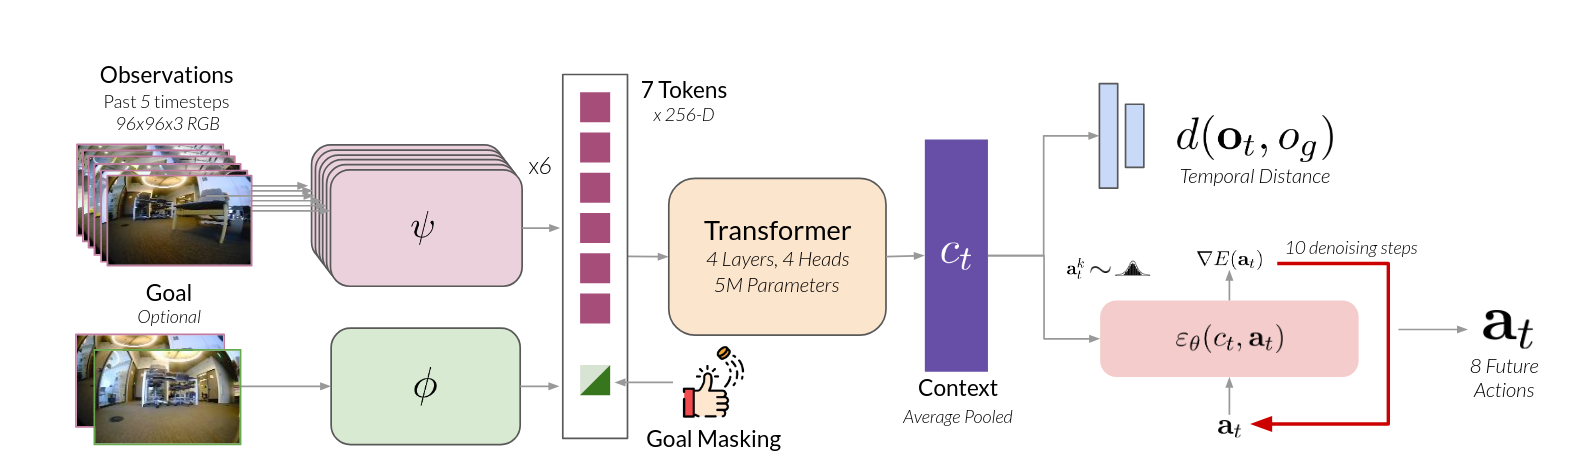
\includegraphics[width=1.01\linewidth]{nomad_diagram.png}
    \end{figure}
\end{frame}

\begin{frame}{Overview of NoMaD Architecture}
    \texttt{NoMaD = \{EfficientNet + Vision Transformer\} $\leftarrow$ \textbf{ViNT} \\+ \textcolor{green}{Diffusion Policies}}\\
    \textbf{Diffusion Policies:}\\
    To model complex, multimodal action distributions, NoMaD employs a diffusion model to approximate the conditional distri-
    bution of the next action as: $p(a_t|c_t)$.\\
    \textbf{1. Forward Process}: Start with a real action $a^{0}_t$ and add gaussian noise to it over multiple steps.
        \begin{center}
            $a^{k}_t = \sqrt{\alpha_k} a^{k-1}_t + (\sqrt{1 - \alpha_k}) \epsilon$
        \end{center}
        where:\\
    \begin{itemize}
        \item $\epsilon$ $\sim$ $\mathcal{N}$(0,I) is a random noise
        \item $\alpha_k$ is a noise scheduler (eg square cosine)
        \item By step K, the action is almost pure noise.
    \end{itemize}
\end{frame}
\begin{frame}{Overview of NoMaD Architecture}
    \texttt{NoMaD = \{EfficientNet + Vision Transformer\} $\leftarrow$ \textbf{ViNT} \\+ \textcolor{green}{Diffusion Policies}}\\
    \textbf{2. Reverse Denoising:} starting from pure noise $a^{k}_t$ $\sim$ $\mathcal{N}(0,I)$, it denoises step by step to recover the final clean action $a^{0}_t$.\\
    Each denoising step is :
    \begin{center}
        \[a^{k-1}_t = \alpha(\alpha^{k}_t-\gamma_k.\epsilon_{\theta}(c_t, a^{k}_t,k)) + \mathcal{N}(0,\sigma^2.I)\]
    \end{center}
    Where:
    \begin{itemize}
        \item Here, $\epsilon_\theta$ is the noise prediction network conditioned on the context $c_t$, which may or may not include the goal depending on $m$.
        \begin{itemize}
            \item It is a 1D conditional U-Net with 15 CNN layers.
            \item Input:Noisy action $a^{k}_t$, Context vector $c_t$, and the diffusion step k.
            \item the predicted noise vector $\hat{\epsilon}_k$,During training, it is compared to the true noise added earlier.
        \end{itemize}
        \item $\gamma, \alpha ,\sigma$ are scheduler constants.
    \end{itemize}
     
\end{frame}

\begin{frame}{Overview of NoMaD Architecture}
    \texttt{NoMaD = \{EfficientNet + Vision Transformer\} $\leftarrow$ \textbf{ViNT} \\+ \textcolor{green}{Diffusion Policies}}\\
    \textbf{3. Action Decoder:} The denoised action $a^{0}_t$ is then passed through a low-level action decoder to generate the final action $a_t$.
    \begin{itemize}
        \item The decoder maps the denoised action to a low-level control command for the robot.
        \item It can be a simple feedforward network or a more complex recurrent network.
    \end{itemize}
    \begin{figure}
        \centering
        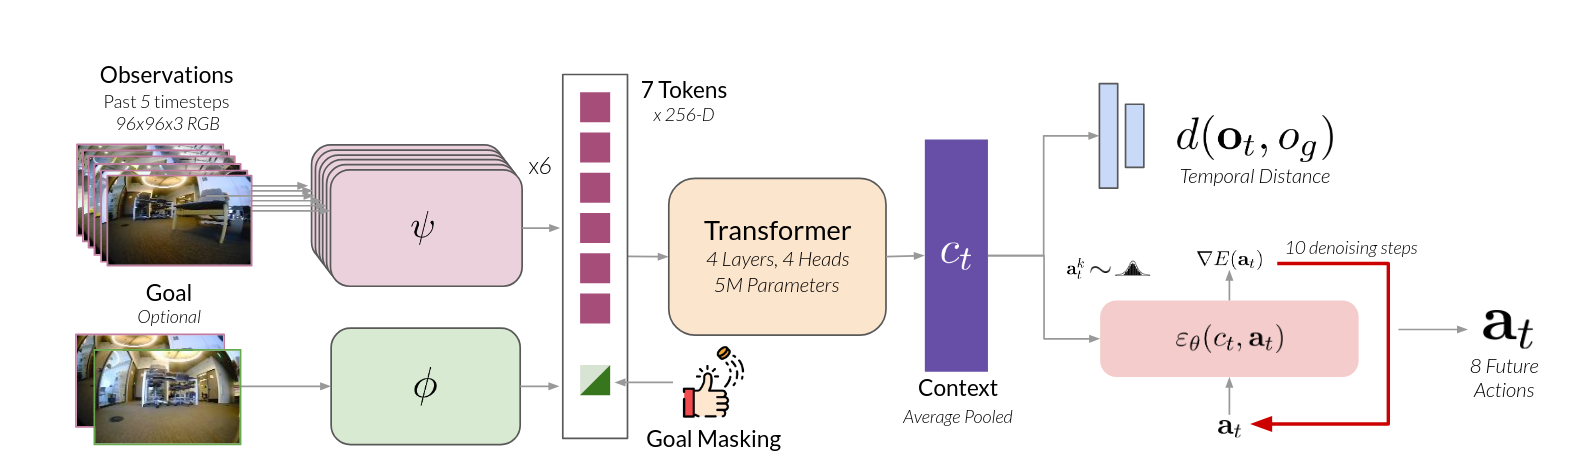
\includegraphics[width=1.01\linewidth]{nomad_diagram.png}
    \end{figure}
\end{frame}

\begin{frame}{Training Details and Experiments}
\begin{itemize}
    \item Datasets used: Sacson/HuRoN, parts of RECON and SCAND
    \item Batch size: 47, Epochs: 10
    \item Optimizer: AdamW, Lr: $10^{-4}$ 
    \item Scheduler: Cosine annealing
\end{itemize}
\begin{figure}
    \centering
    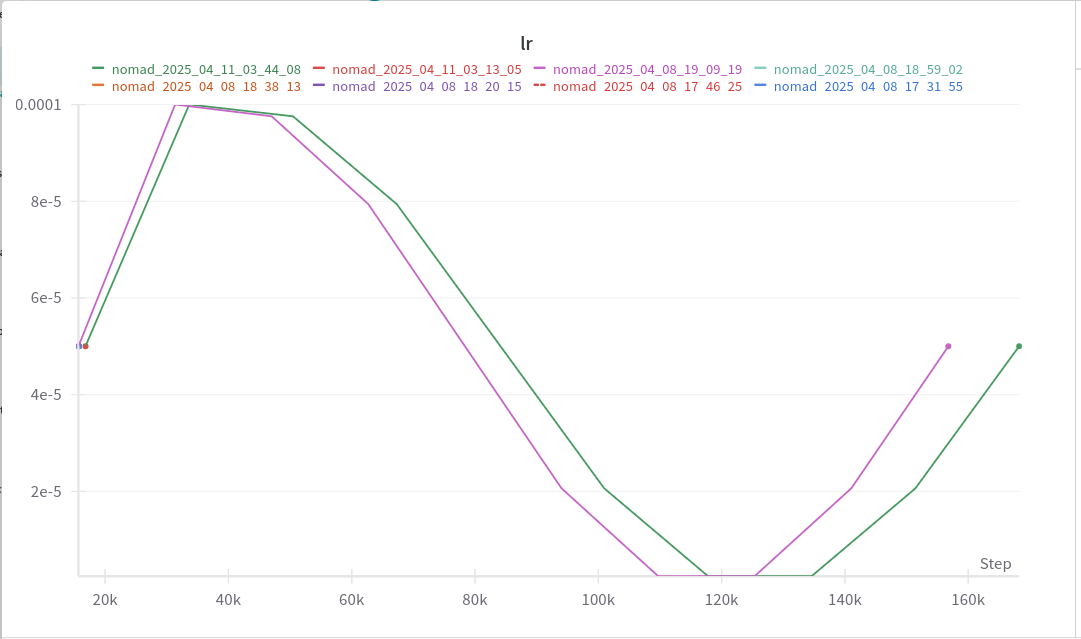
\includegraphics[width=0.8\linewidth]{lrdecay.png}
    \caption{Lr decay using cosine annealing}
    \label{fig:lrdecay}
\end{figure}
\end{frame}
\begin{frame}{Training Details and Experiments}
    \begin{itemize}
        \item Goal Masking Probability: $p_m$ = 0.5
        \item Diffusion Steps: 10
        \item Noise Scheduler: Square Cosine
    \end{itemize}
    \pause
    \begin{block}{Training Objective}
        \begin{itemize}
            \item \textbf{Diffusion Loss:} Measures the difference between the predicted and true noise.
            \item \textbf{Distance Loss:} Measures the difference between the predicted and true distance to the goal.
        \end{itemize}
    \end{block}
    \[ \mathcal{L}_{NoMaD}(\phi,\psi,f,\theta,f_d) = MSE(\epsilon^{k}, \epsilon_{\theta}(c_t, a^{0}_t + \epsilon^{k},k)) + \lambda .MSE(d(o_t, o_g), f_{d}(c_t))\]
    where:\\
    \begin{itemize}
        \item We set $\lambda$ to $10^{-4}$
        \item $\psi$,\ $\phi$ correspond to the visual encoders for the observation and goal images.
        \item $f$ corresponds to the transformer layers, $\theta$ to diffusion parameters,
        \item $f_d$ corresponds to the temporal distance predictor.
    \end{itemize}
\end{frame}

\begin{frame}{Training Visualization with \texttt{wandb}}

    \begin{block}{Why \texttt{Weights \& Biases (wandb)}?}
        We used \texttt{wandb} to log training progress, visualize losses, and monitor both model behavior and system resources (e.g., GPU/CPU utilization) throughout experimentation. 
        Metrics such as \textbf{action loss}, \textbf{goal prediction error}, and the \textbf{learning rate schedule} were automatically tracked and visualized, 
        which helped with debugging and plotting out results.
    \end{block}

    \begin{columns}
        \begin{column}{0.4\textwidth}
            \begin{figure}
                
\includegraphics[width=0.5\textwidth]{images/qr_project.png}
                \caption{QR code to project webpage}
            \end{figure}
        \end{column}
        \begin{column}{0.6\textwidth}
            \begin{figure}
                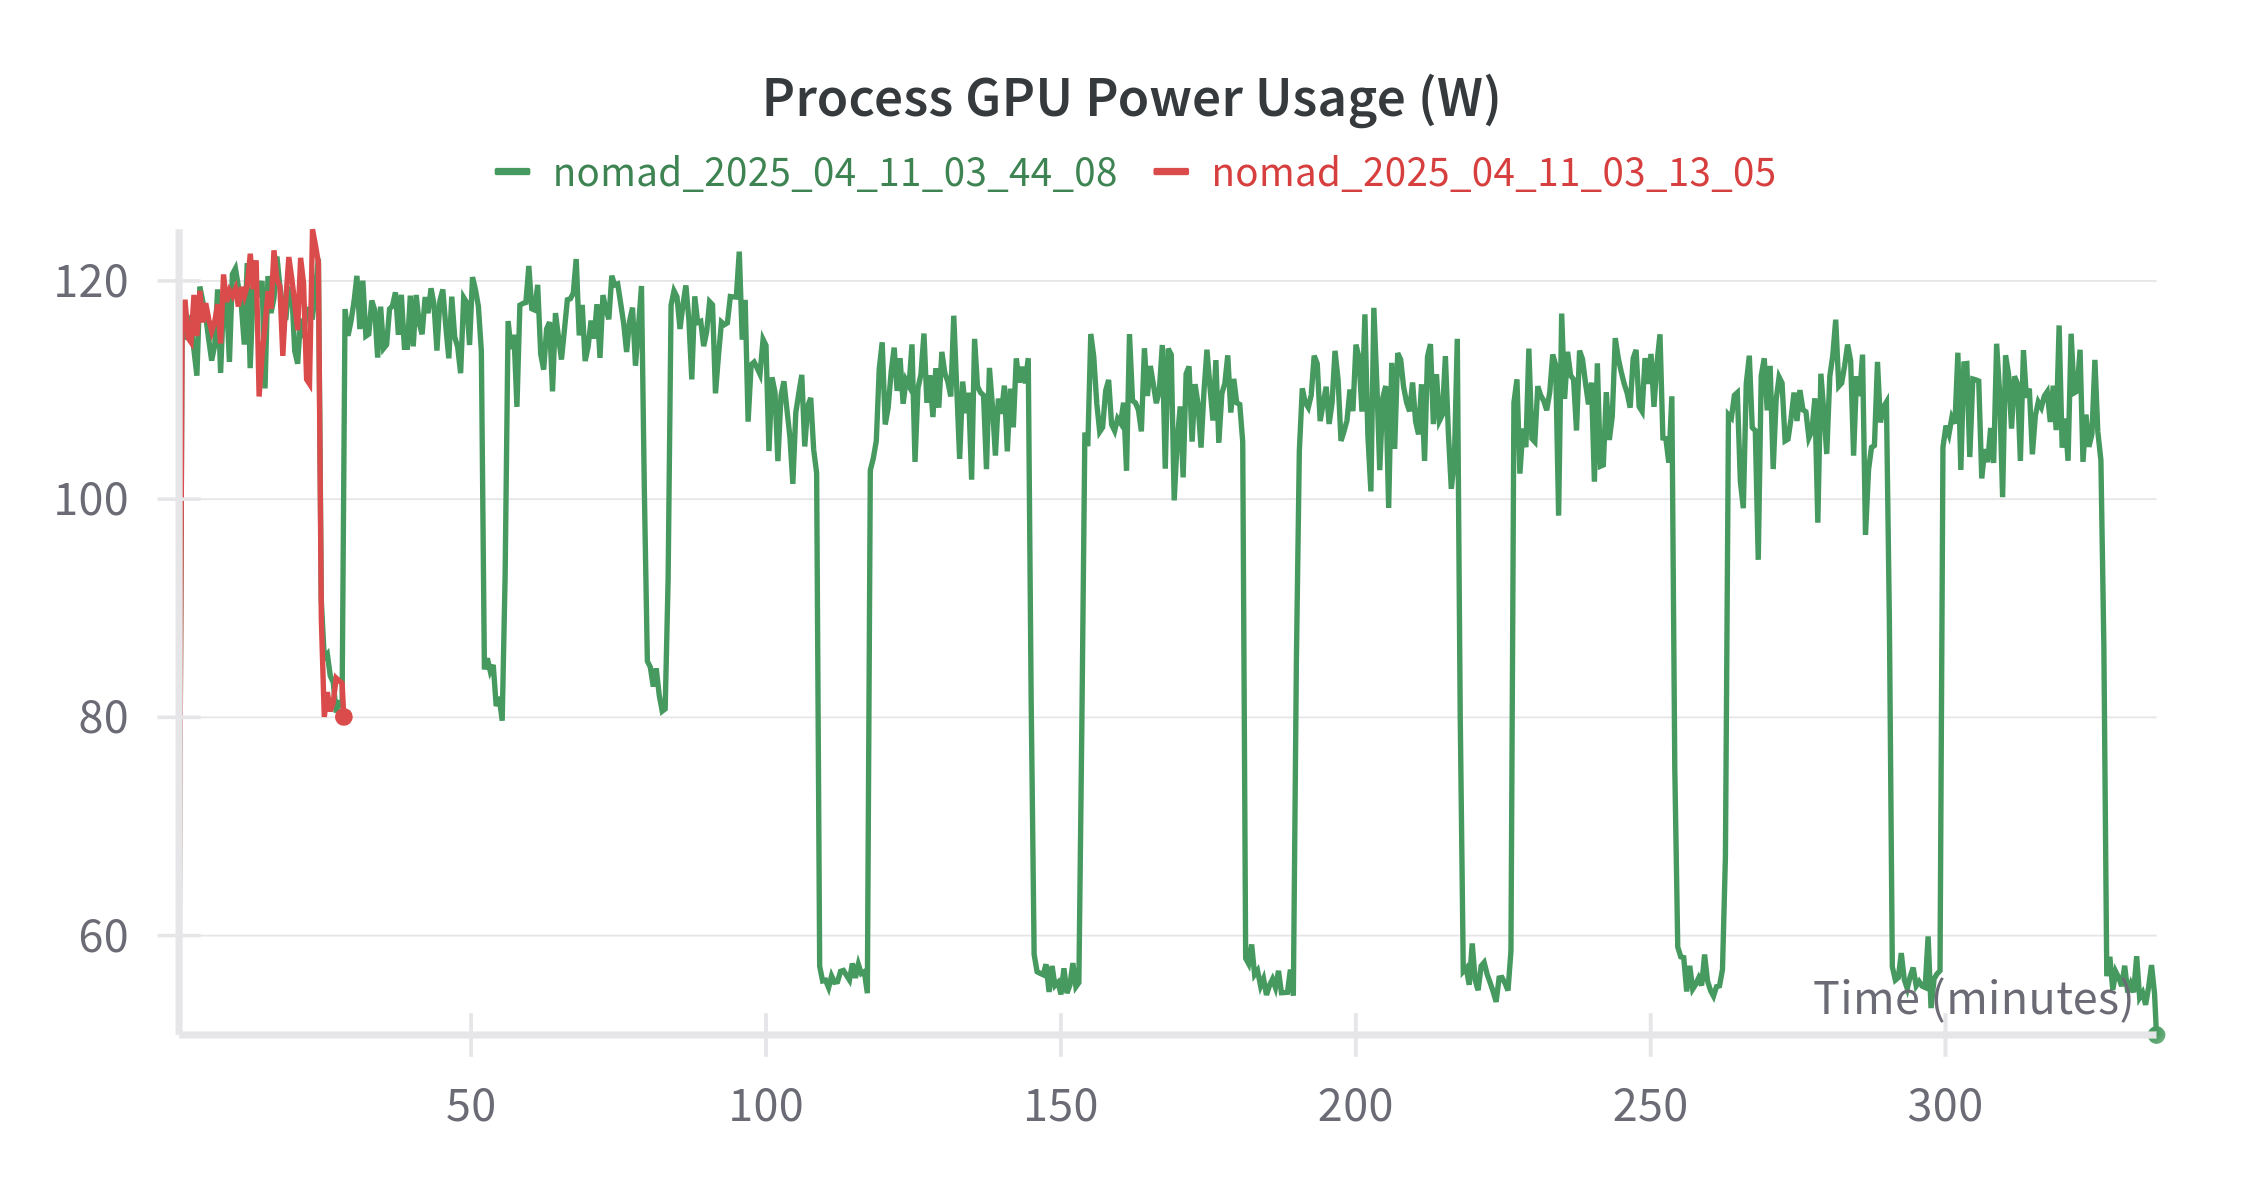
\includegraphics[width=0.8\textwidth]{images/gpu_powerusage.png}
                \caption{GPU power usage during training}
            \end{figure}
        \end{column}
    \end{columns}

\end{frame}
\begin{frame}{Action Samples generated by NoMaD}
The figure illustrates a robot is trying to navigate towards a specific goal.\\
\begin{itemize}
    \item The left plot shows action trajectories sampled by the diffusion model in 2D space.
    \item Green and red lines represent different stages of the diffusion process (noisy vs. denoised).
    \item The pink line shows the final selected action sequence
\end{itemize}    
    \begin{block}{During Training}
        \begin{figure}
            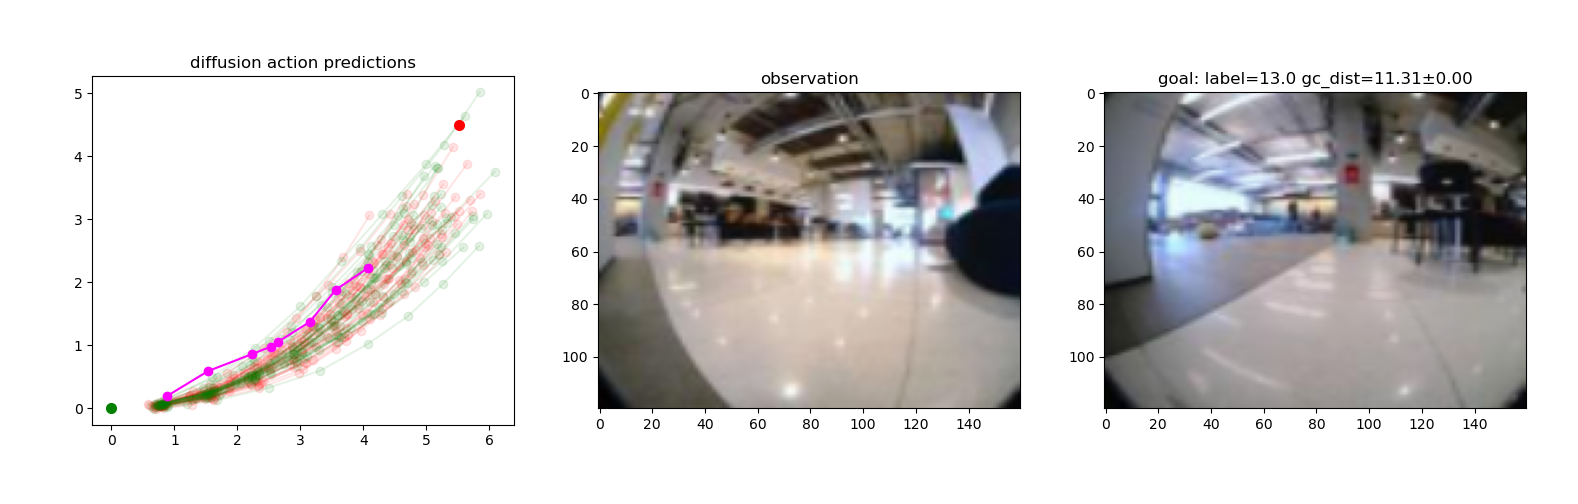
\includegraphics[width=1\linewidth]{images/train_action_samples_2.png}        \end{figure}
    \end{block}
\end{frame}
\begin{frame}{Action Samples generated by NoMaD}
    The figure illustrates a robot is trying to navigate towards a specific goal.\\
    \begin{itemize}
        \item The left plot shows action trajectories sampled by the diffusion model in 2D space.
        \item Green and red lines represent different stages of the diffusion process (noisy vs. denoised).
        \item The pink line shows the final selected action sequence
    \end{itemize}    
    \begin{block}{During Testing}
        \begin{figure}
            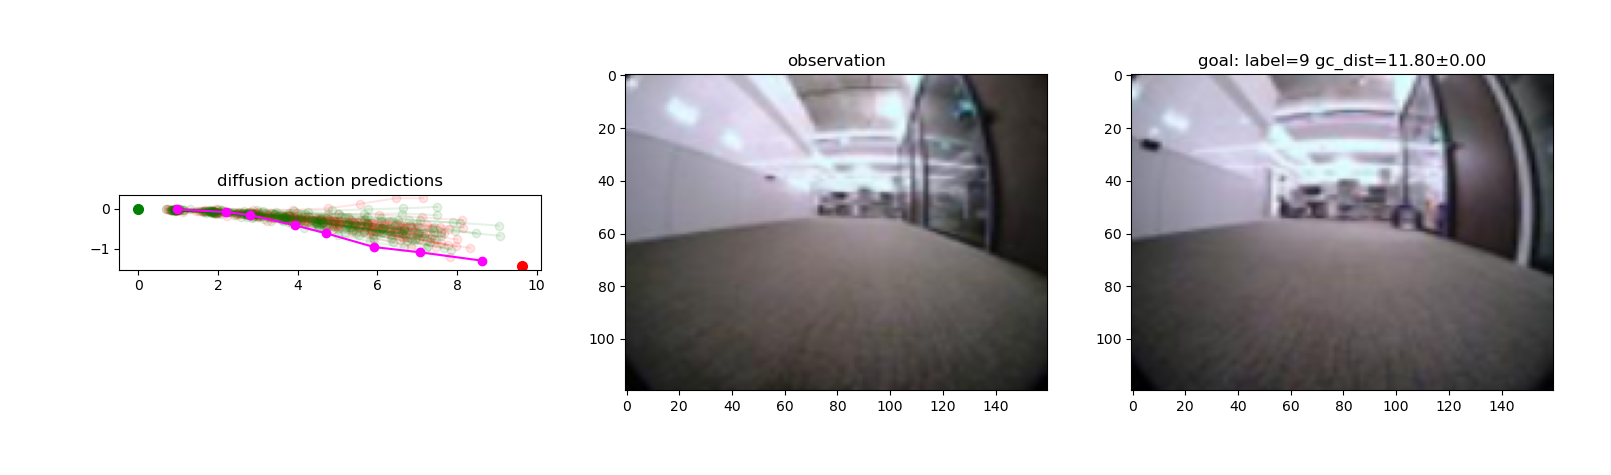
\includegraphics[width=1\linewidth]{images/sacson_test_action_samples_1.png}        \end{figure}
    \end{block}
\end{frame}
\begin{frame}{Experiments and Results: (Goal Conditioned)}
We set the goal mask $m = 0$ to evaluate the model's performance in goal-directed navigation.
\begin{block}{Distance Loss}
    \begin{figure}[H]
        \centering
        \begin{subfigure}[b]{0.48\textwidth}
            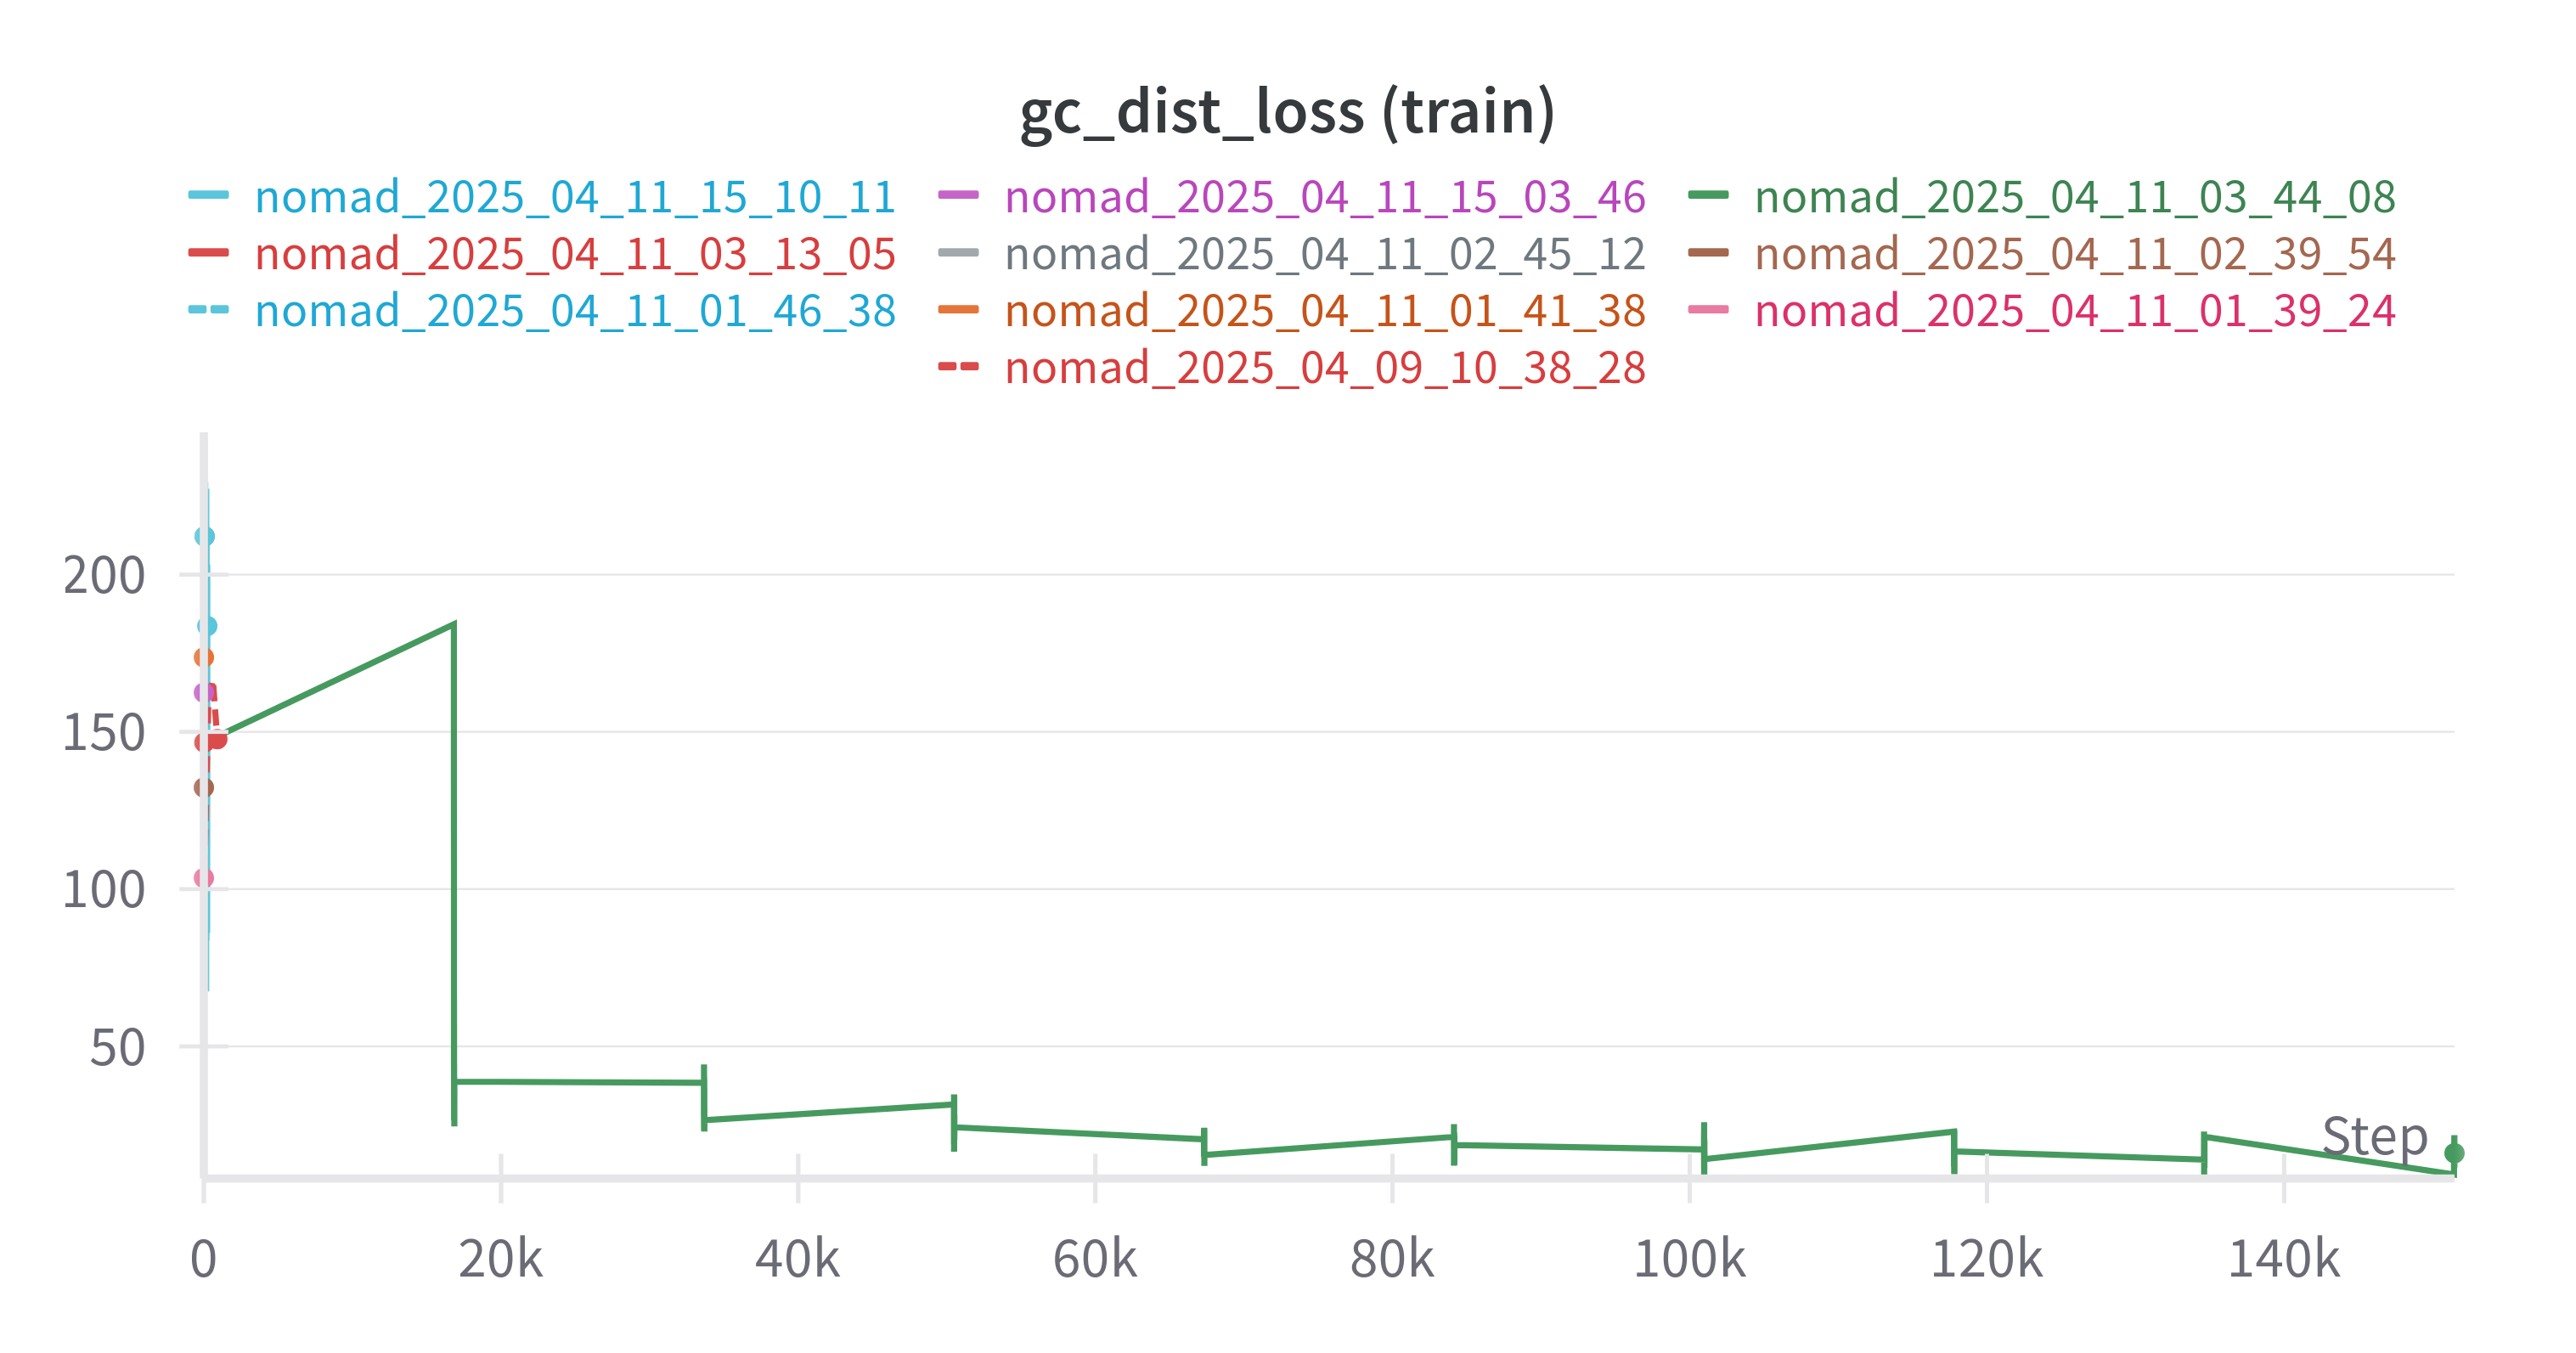
\includegraphics[width=\textwidth]{images/gc_distloss_nomad.png}
            \caption{Distance Loss on Training Set}
            \label{fig:gc_dist_loss_train}
        \end{subfigure}
        \hfill
        \begin{subfigure}[b]{0.48\textwidth}
            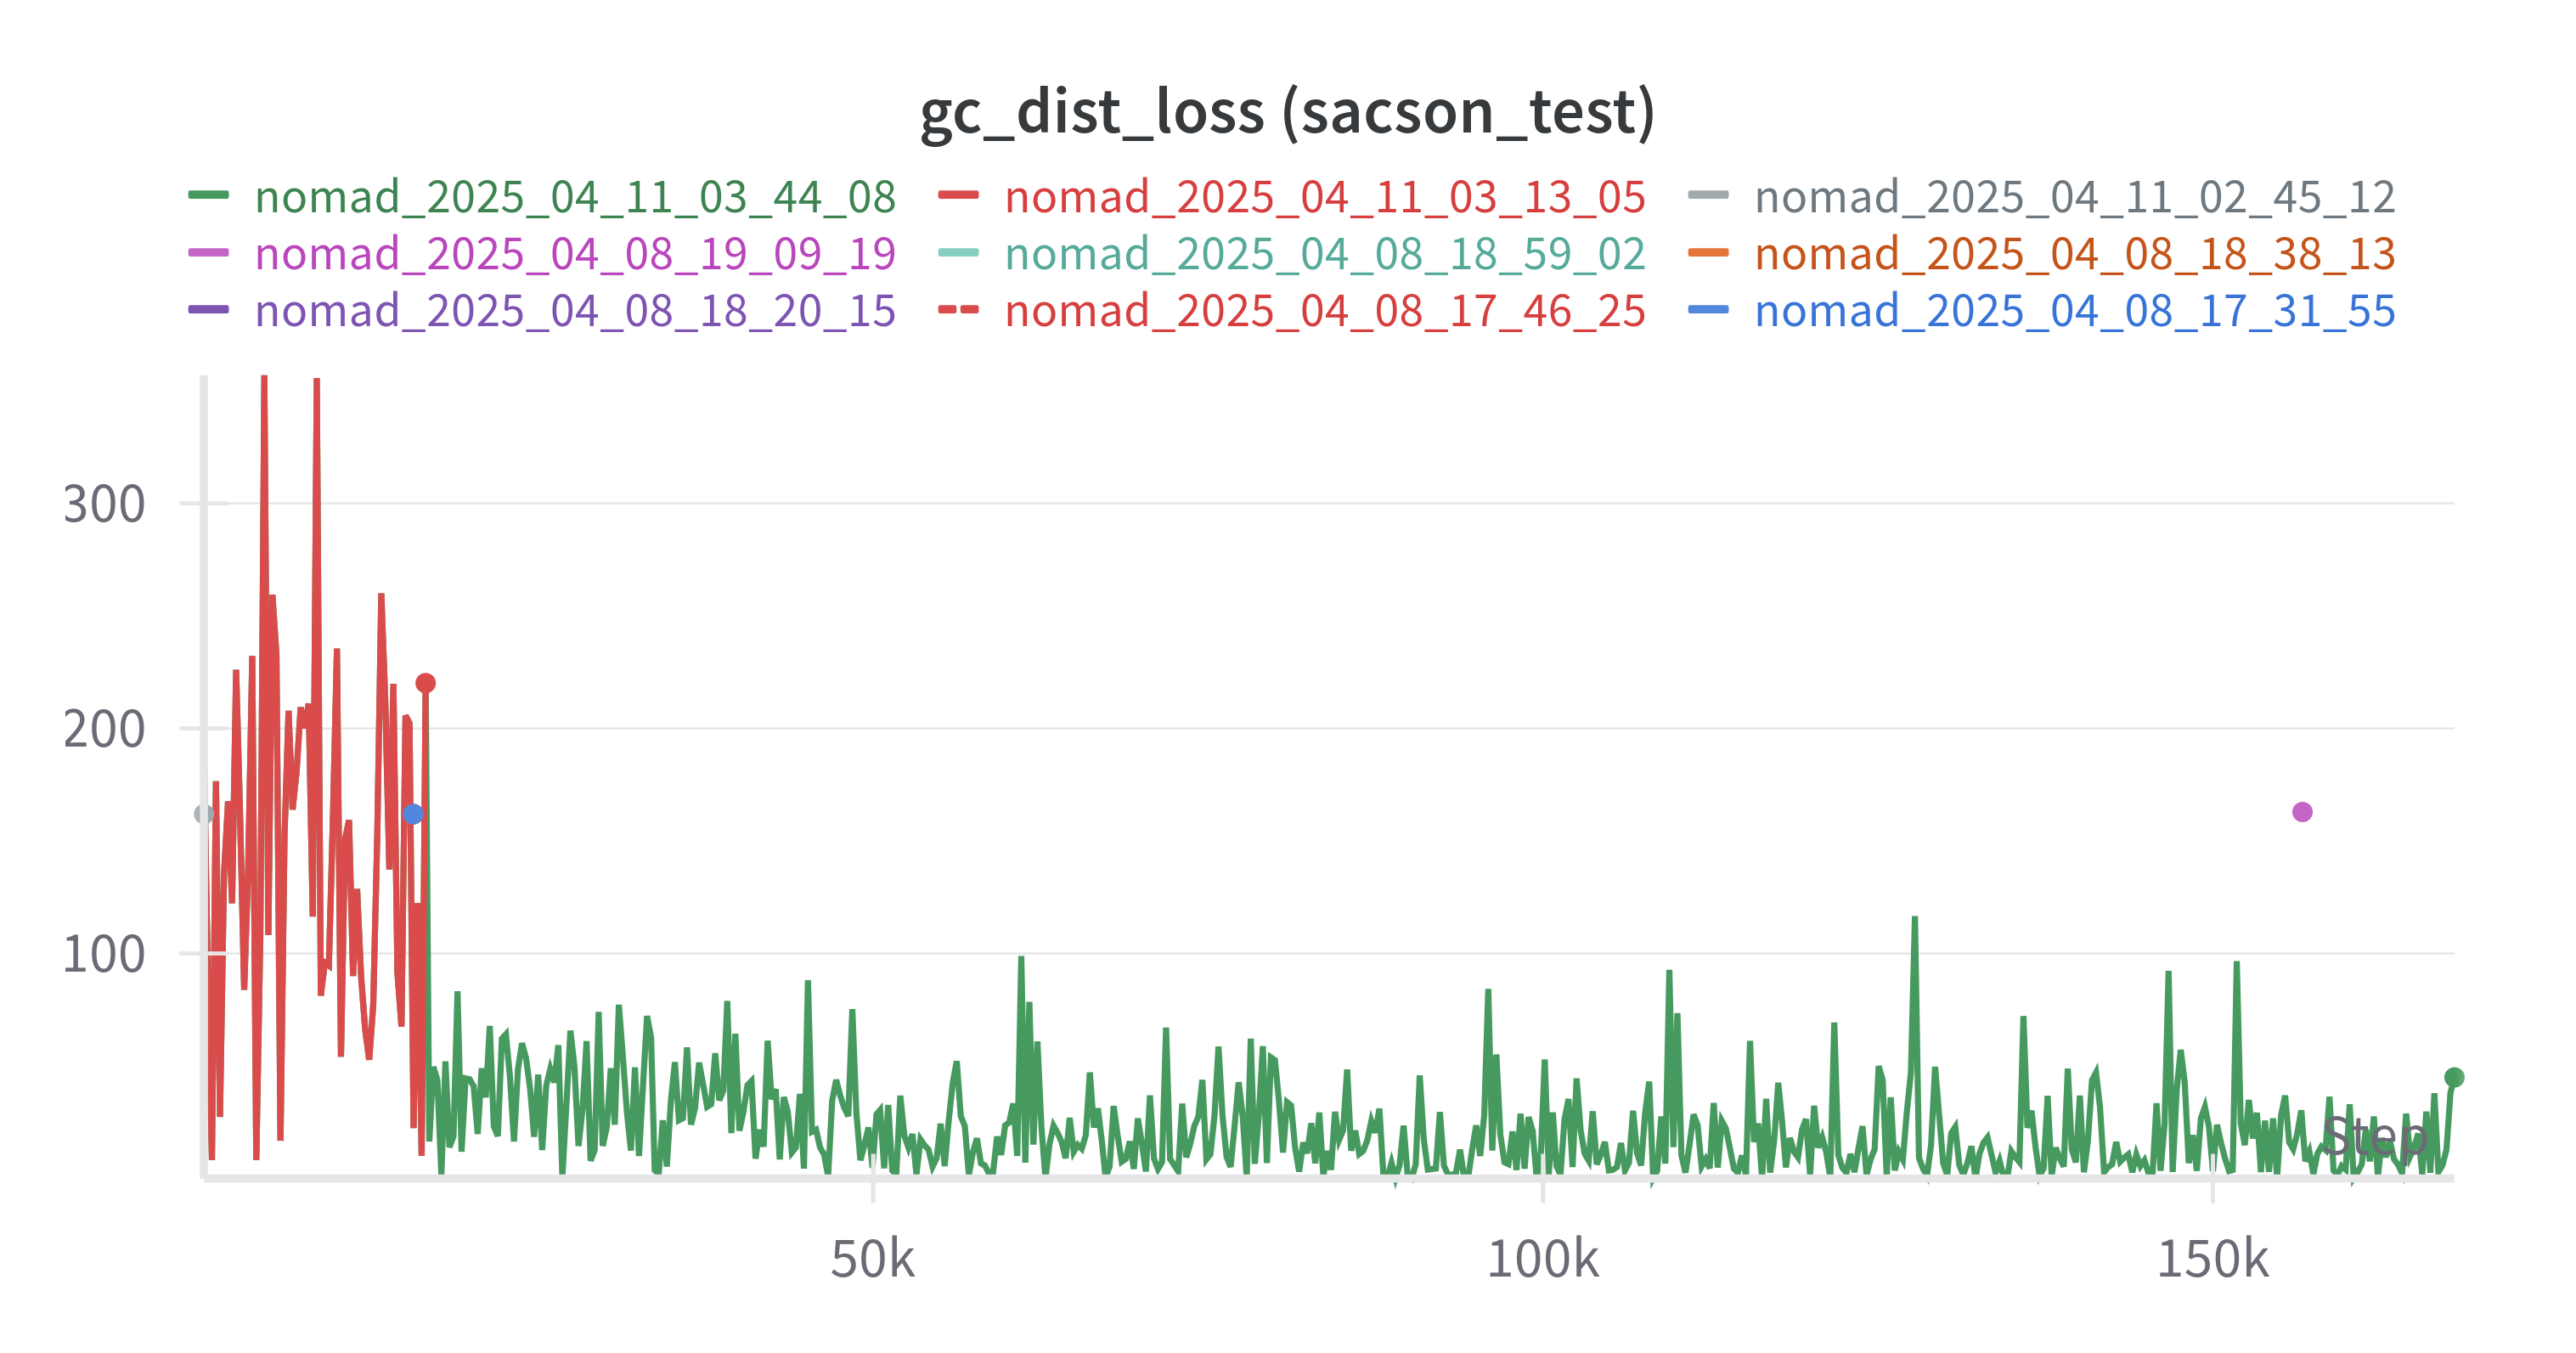
\includegraphics[width=\textwidth]{images/gc_dist_loss_test.png}
            \caption{Distance Loss on Validation Set}
            \label{fig:gc_dist_loss_val}
        \end{subfigure}
        \caption{Distance loss comparison between training and validation sets under goal-conditioned evaluation.}
    \end{figure}
\end{block}

\end{frame}
\begin{frame}{Experiments and Results: (Goal Conditioned)}
We set the goal mask $m = 0$ to evaluate the model's performance in goal-directed navigation.
    \begin{block}{Action Loss}
        \begin{figure}[H]
            \centering
            \begin{subfigure}[b]{0.48\textwidth}
                \centering
                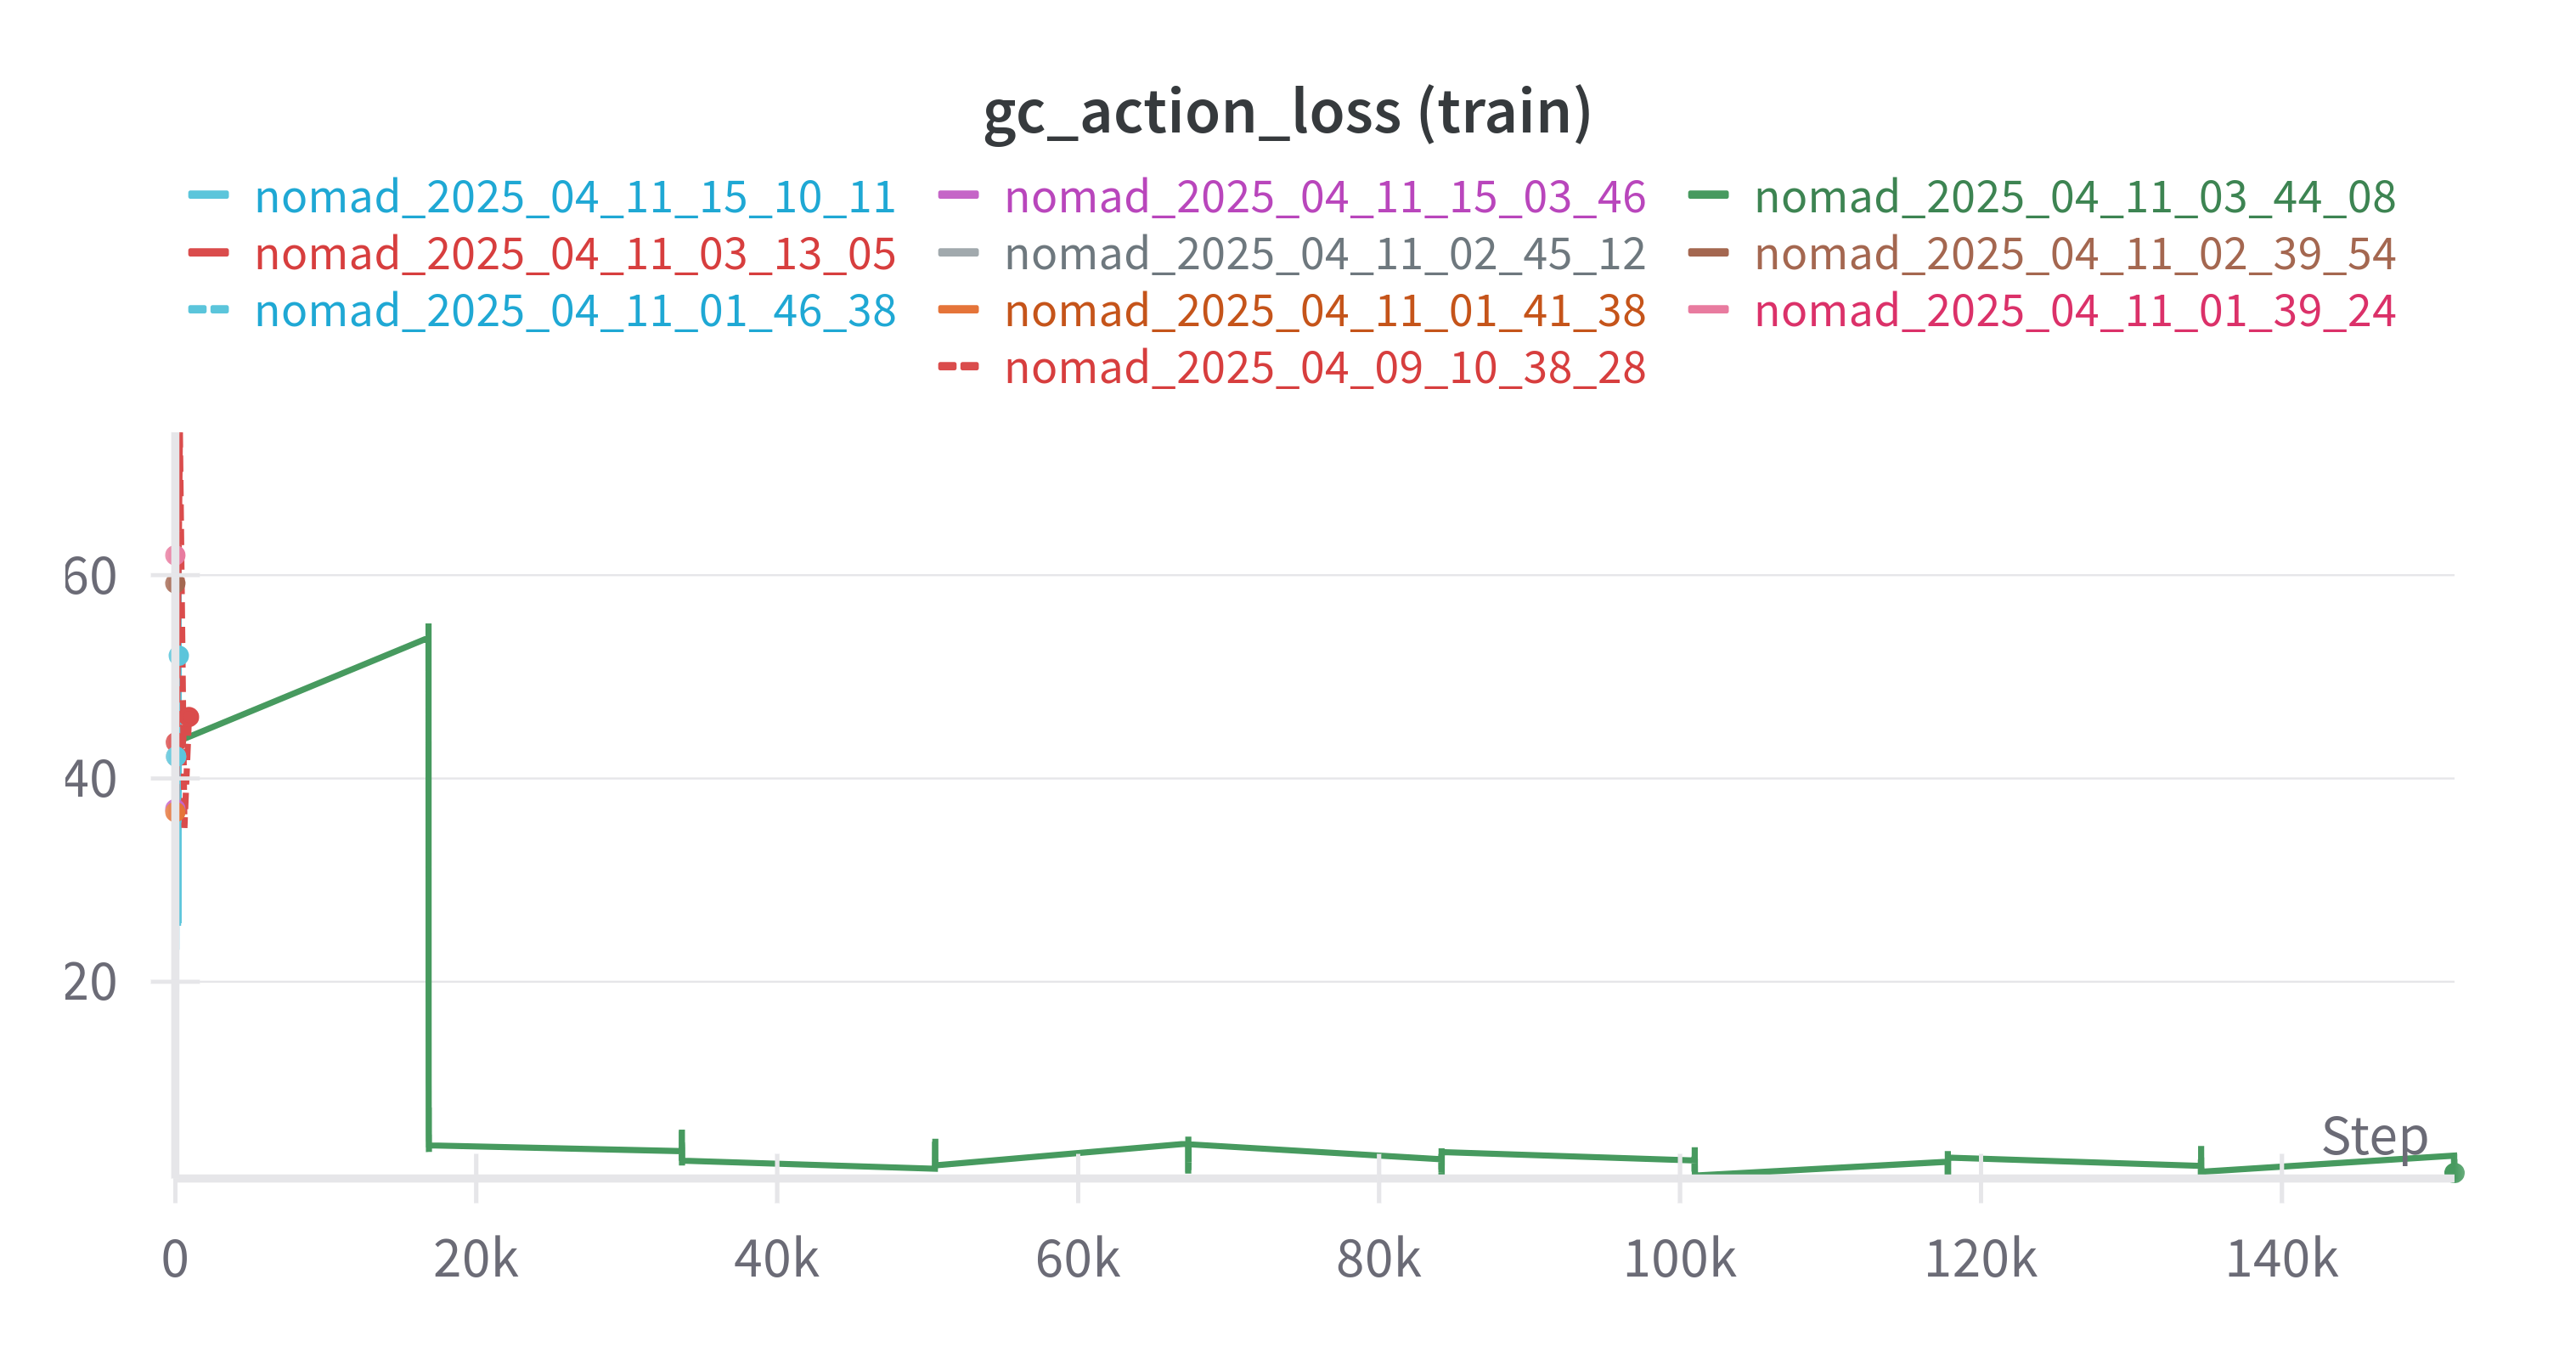
\includegraphics[width=\textwidth]{images/gc_actionloss_nomad.png}
                \caption{Action Loss on Training Set}
                \label{fig:gc_action_loss_train}
            \end{subfigure}
            \hfill
            \begin{subfigure}[b]{0.48\textwidth}
                \centering
                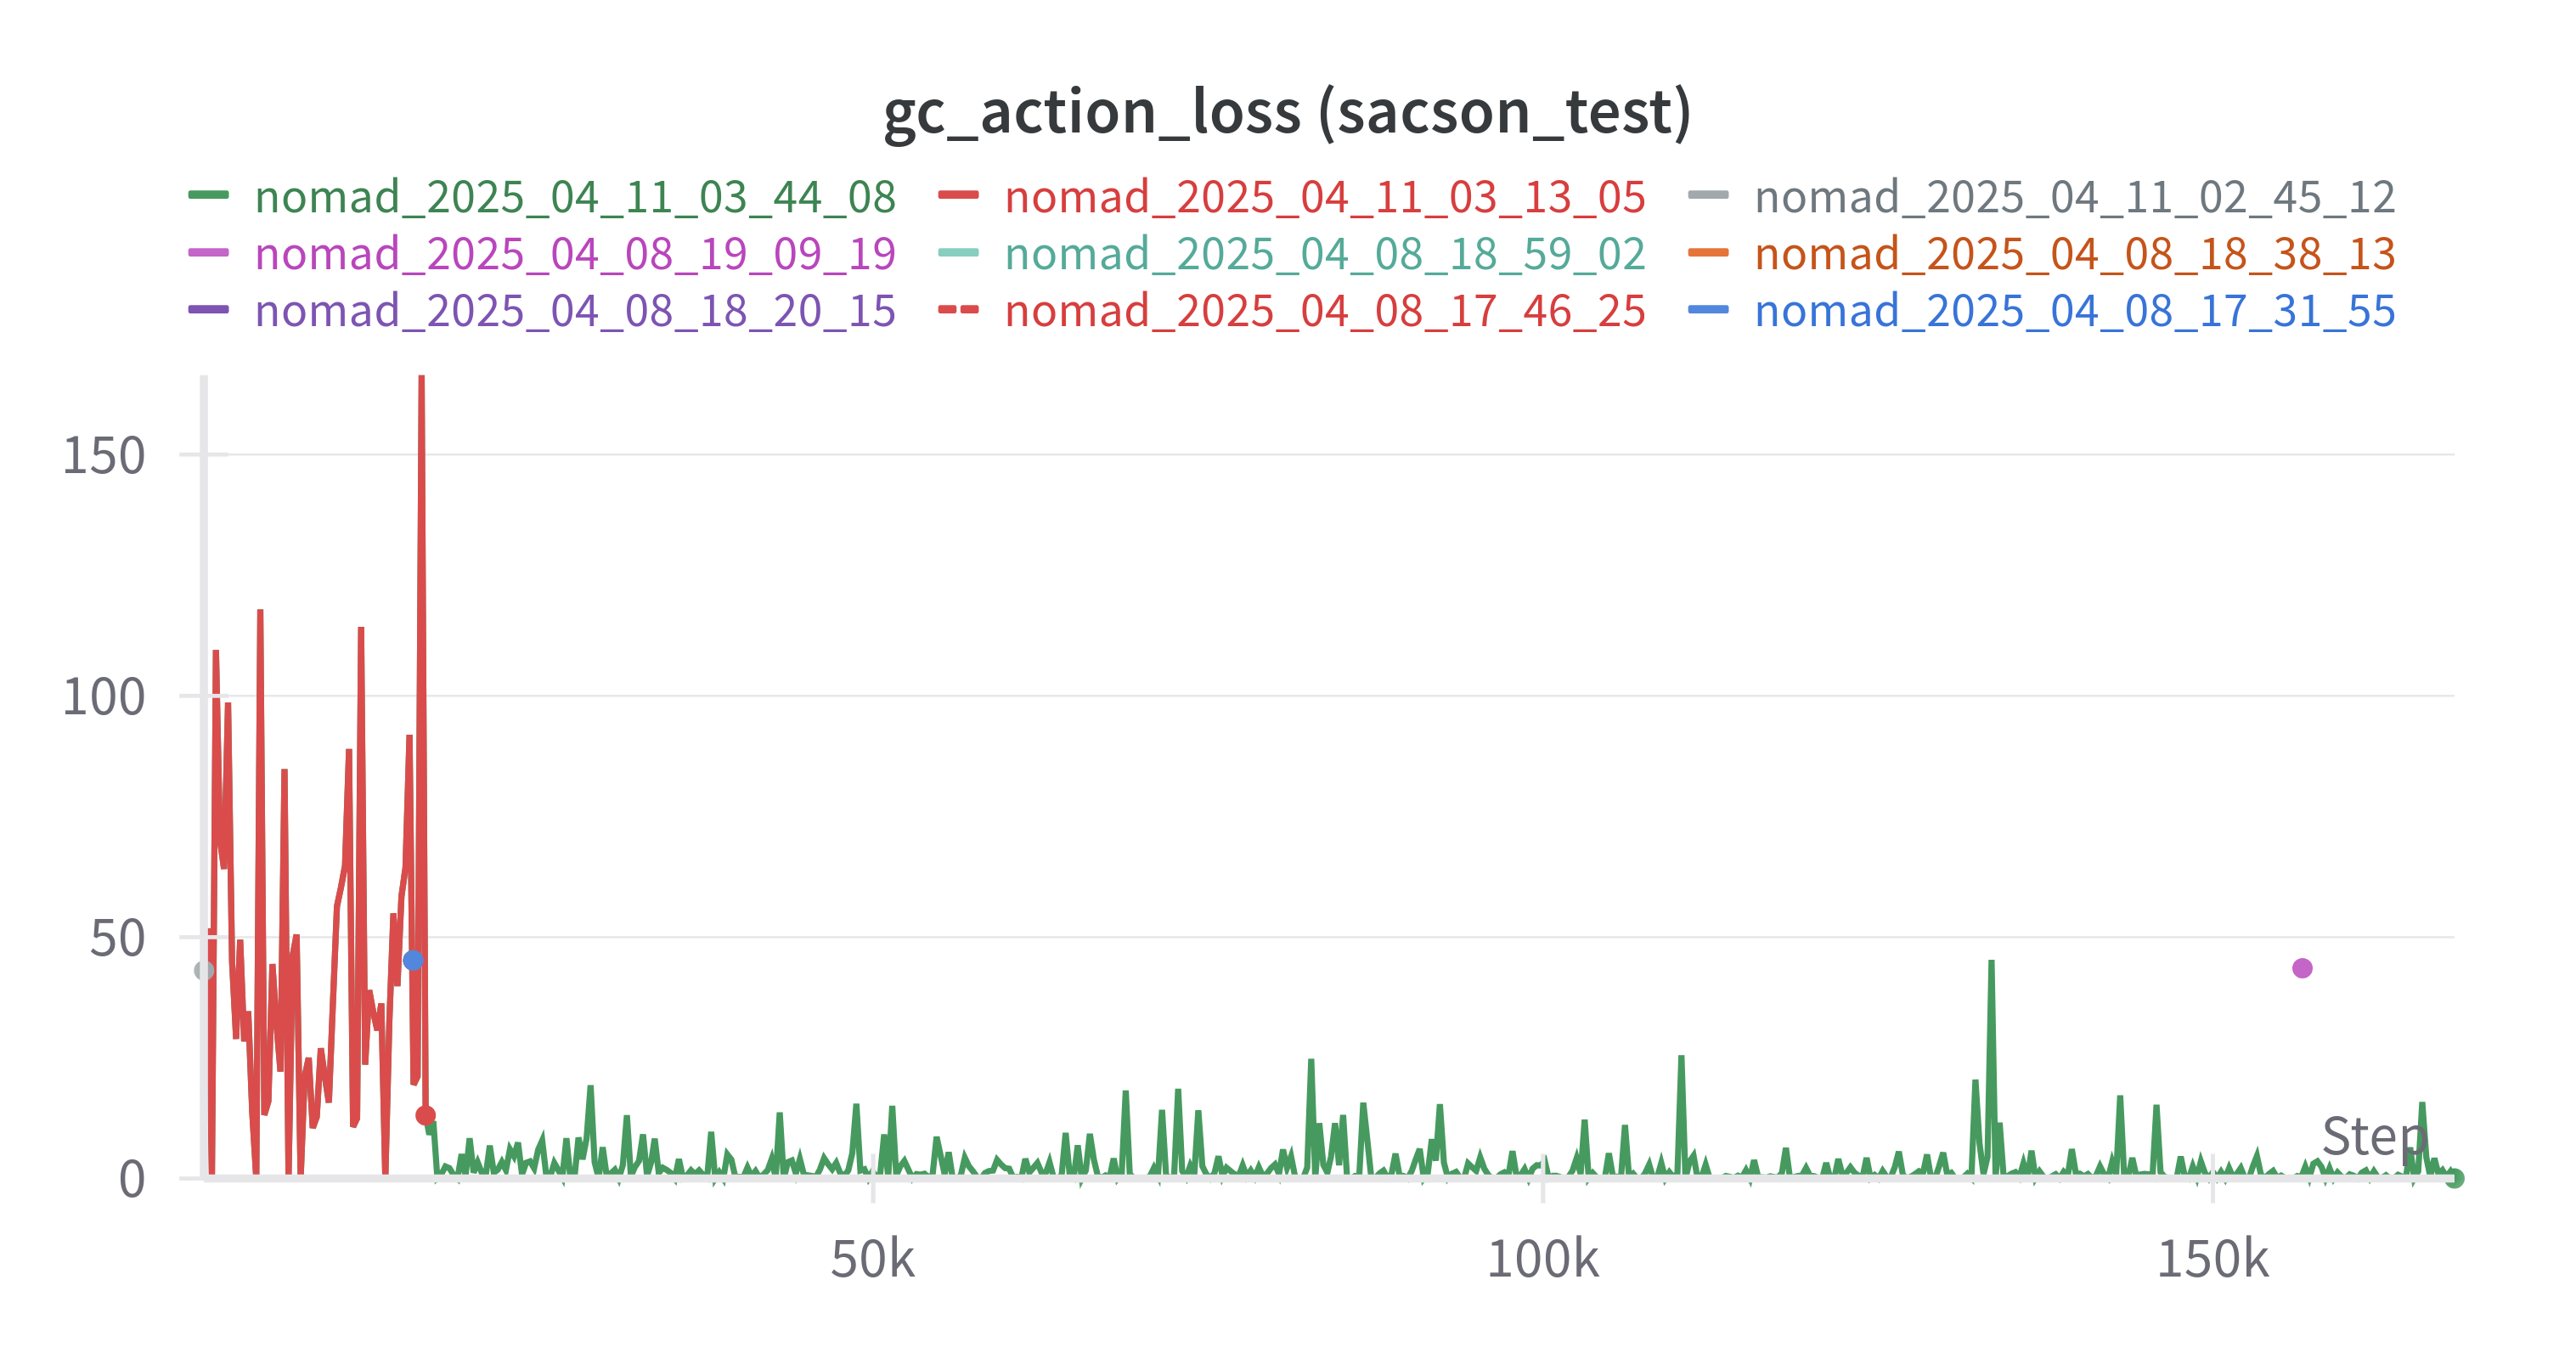
\includegraphics[width=\textwidth]{images/gc_actionloss_test_nomad.png}
                \caption{Action Loss on Validation Set}
                \label{fig:gc_action_loss_val}
            \end{subfigure}
            \caption{Action loss comparison between training and validation sets under goal-conditioned evaluation.}
        \end{figure}
    \end{block}
    \end{frame}
    \begin{frame}{Experiments and Results: (Unconditioned Setting)}
        \begin{block}{Action Loss Evaluation}
            \begin{minipage}{0.48\textwidth}
                \centering
                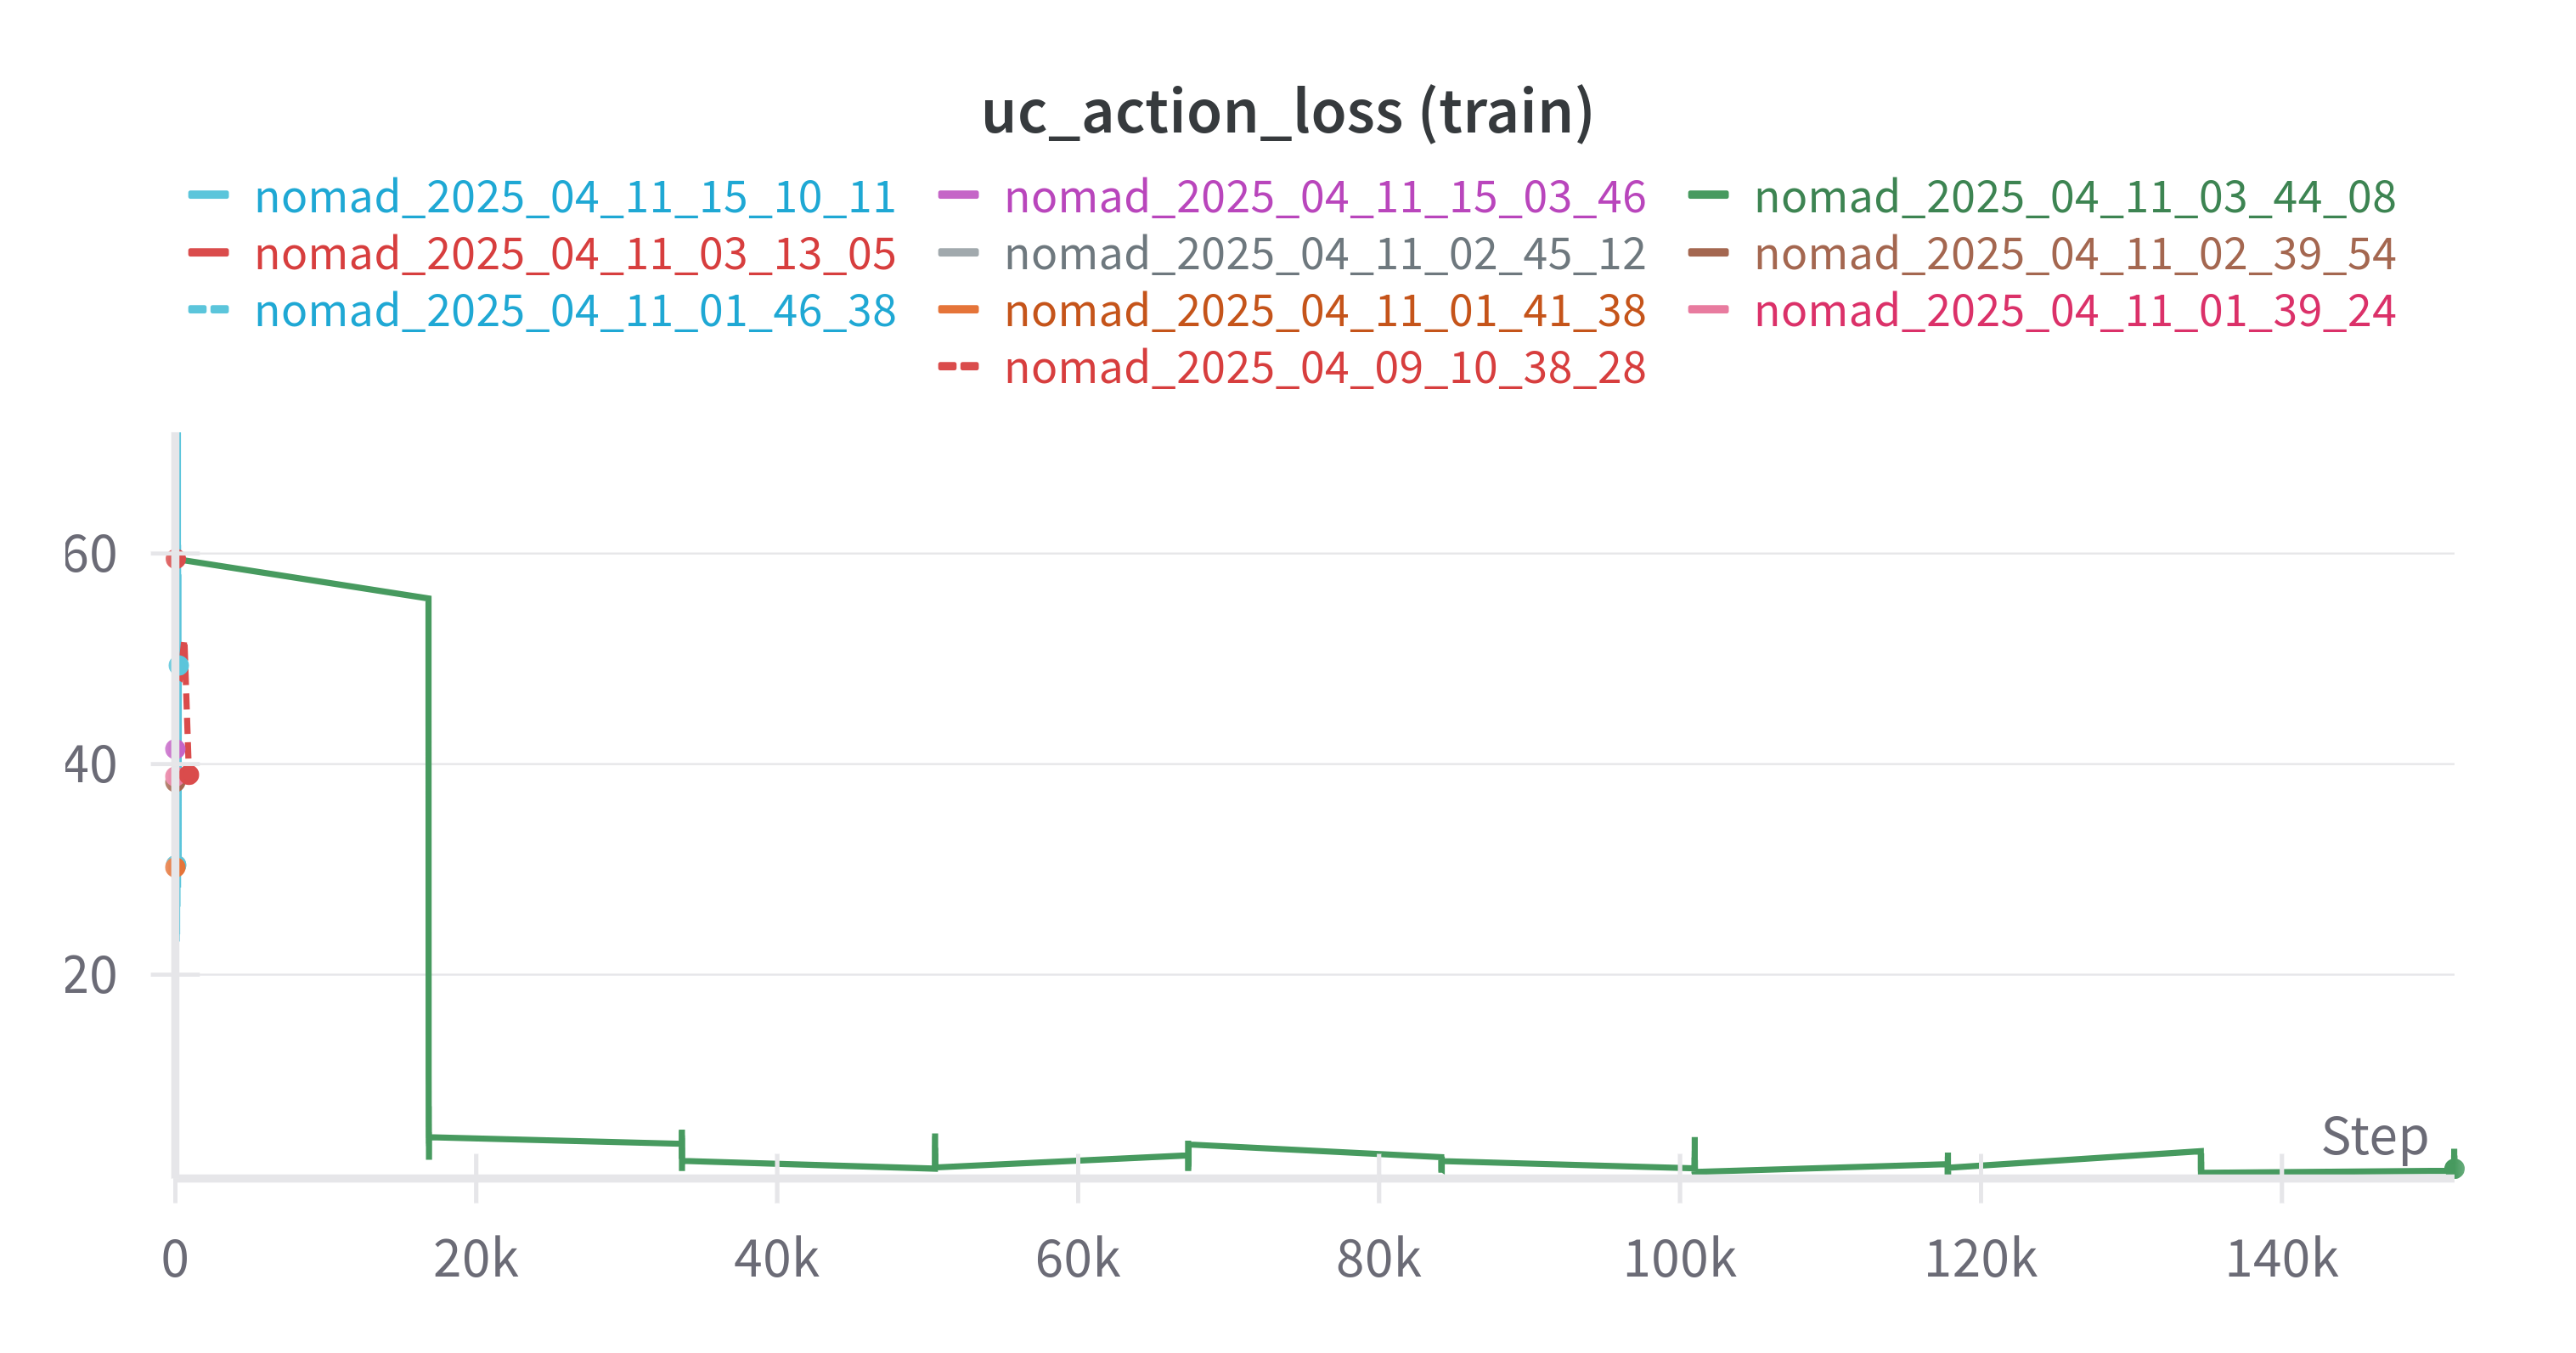
\includegraphics[width=\textwidth]{images/uc_action_train.png}
                
                \textbf{Training Set}
            \end{minipage}
            \hfill
            \begin{minipage}{0.48\textwidth}
                \centering
                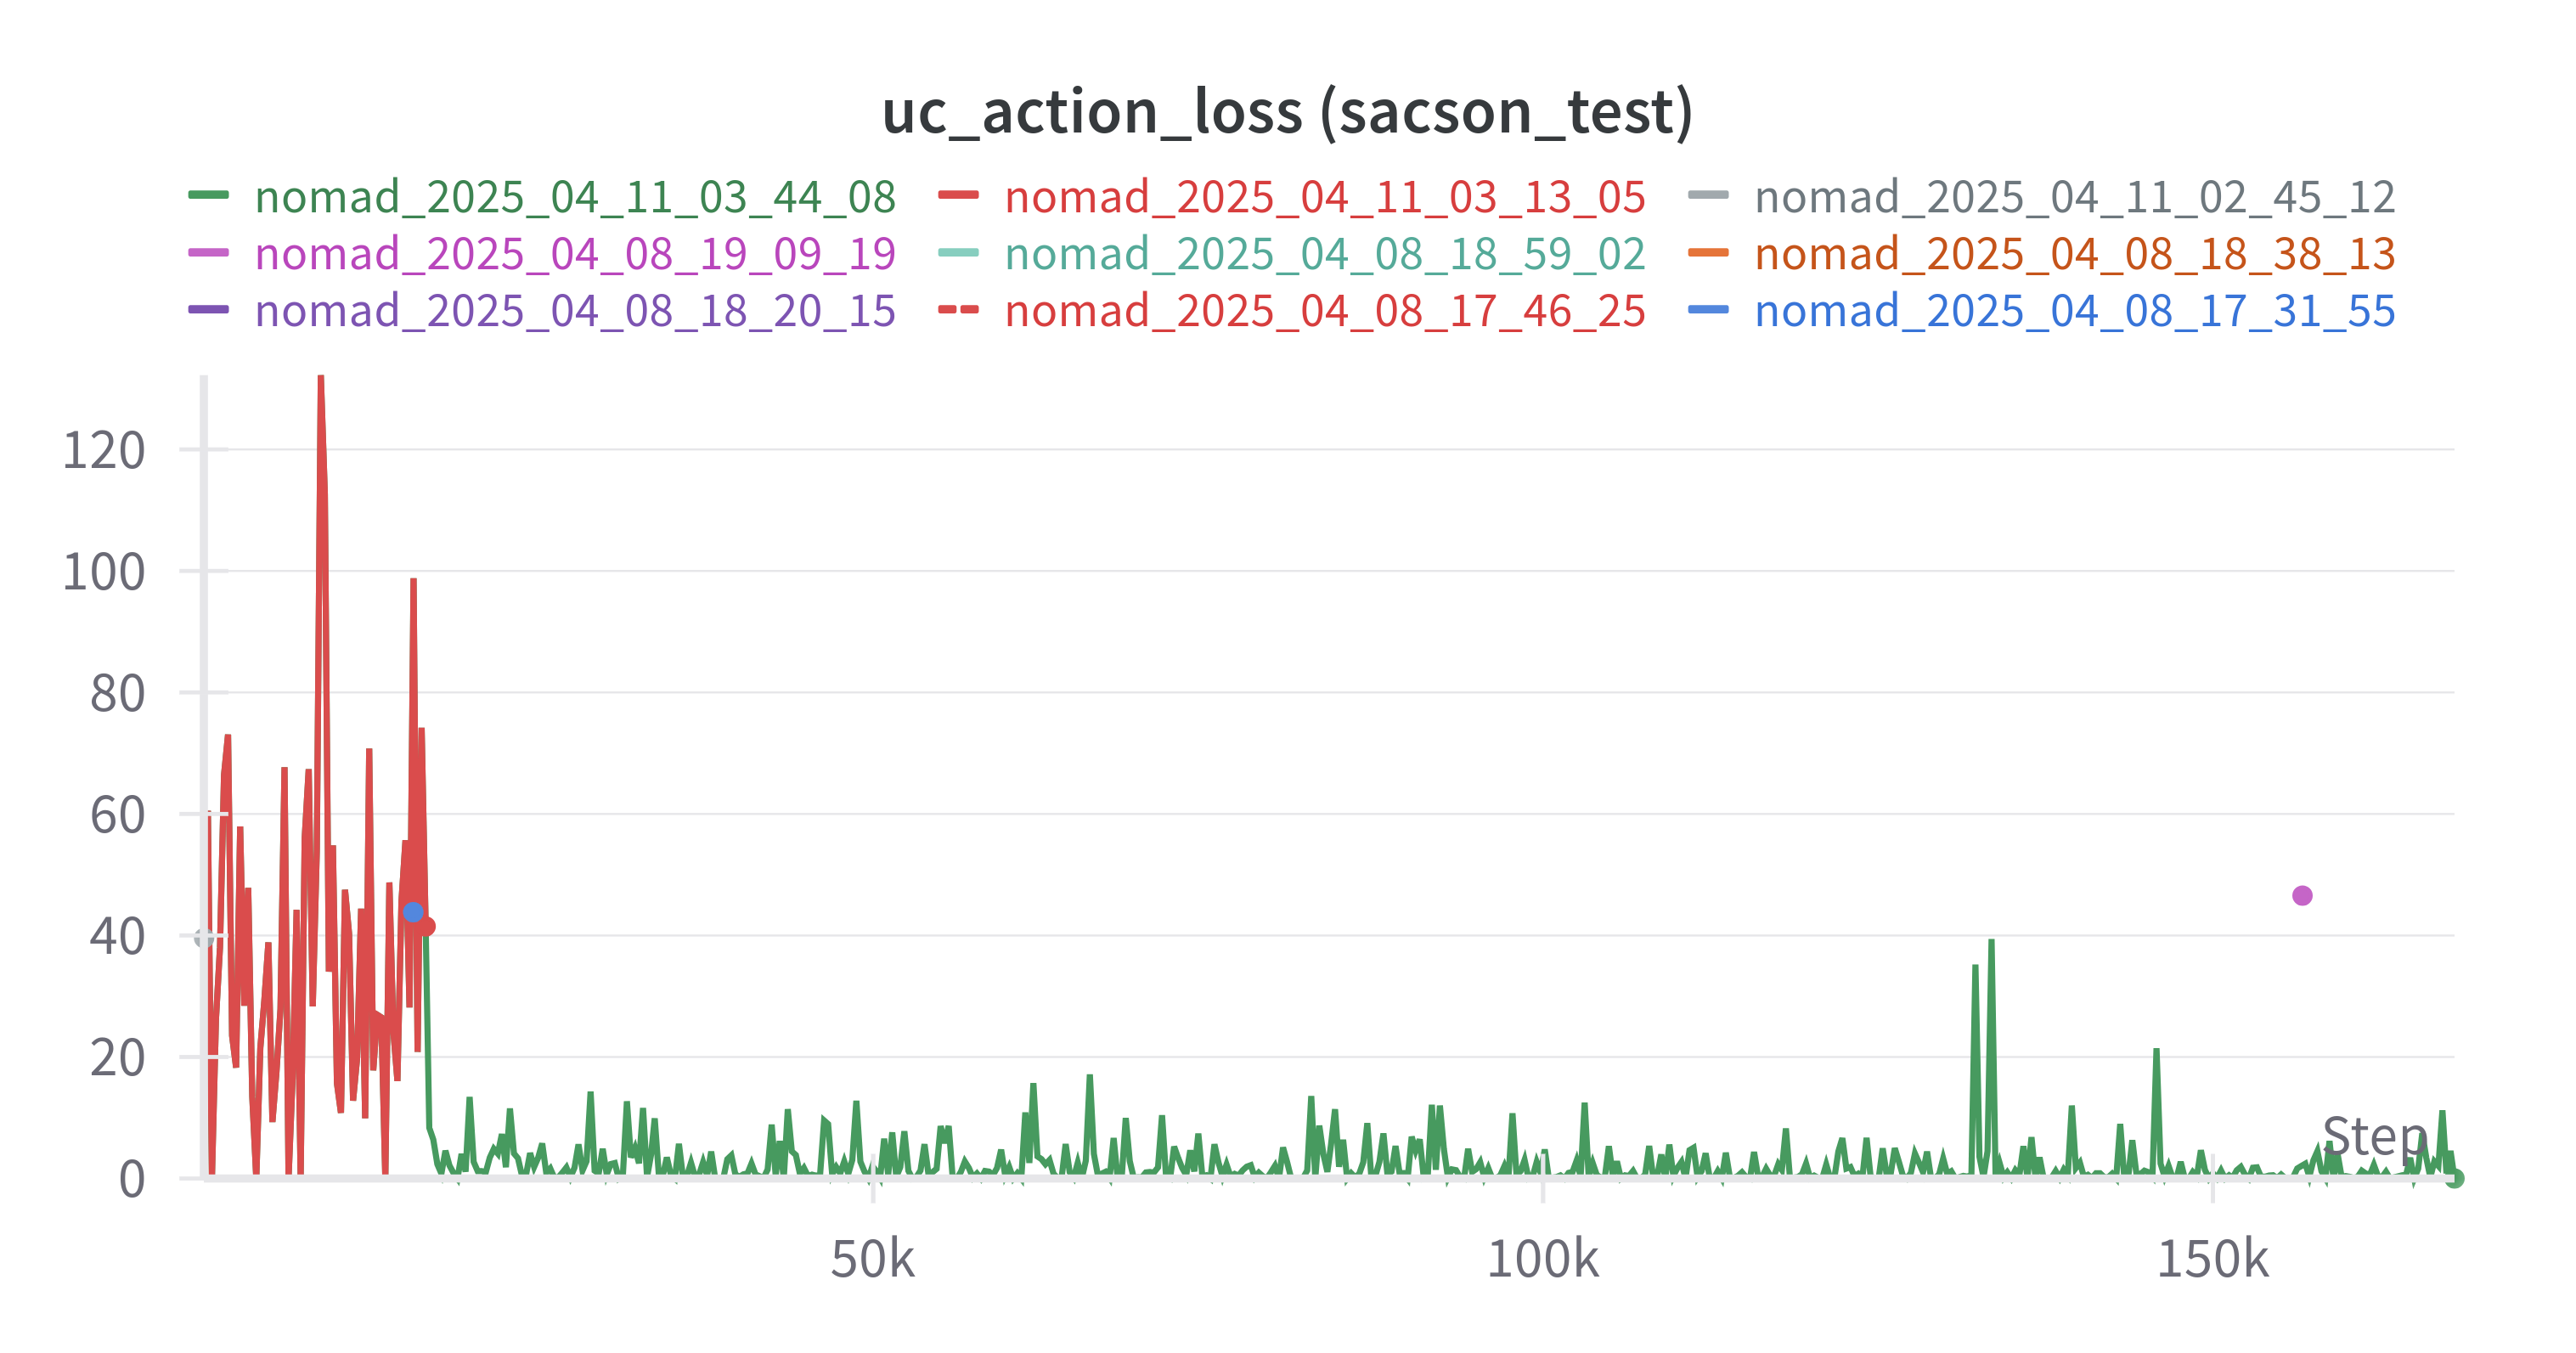
\includegraphics[width=\textwidth]{images/uc_action_test.png}
                
                \textbf{Validation Set}
            \end{minipage}
            
            \vspace{0.5em}
            \bigskip
            The unconditioned action loss measures model accuracy in open-loop, goal-agnostic settings. Lower loss indicates better generalization in exploratory behavior.
        \end{block}
    \end{frame}
    \begin{frame}{Experiments and Results: Distance and Diffusion Losses}
        \begin{block}{Overall Metrics}
            \begin{minipage}{0.48\textwidth}
                \centering
                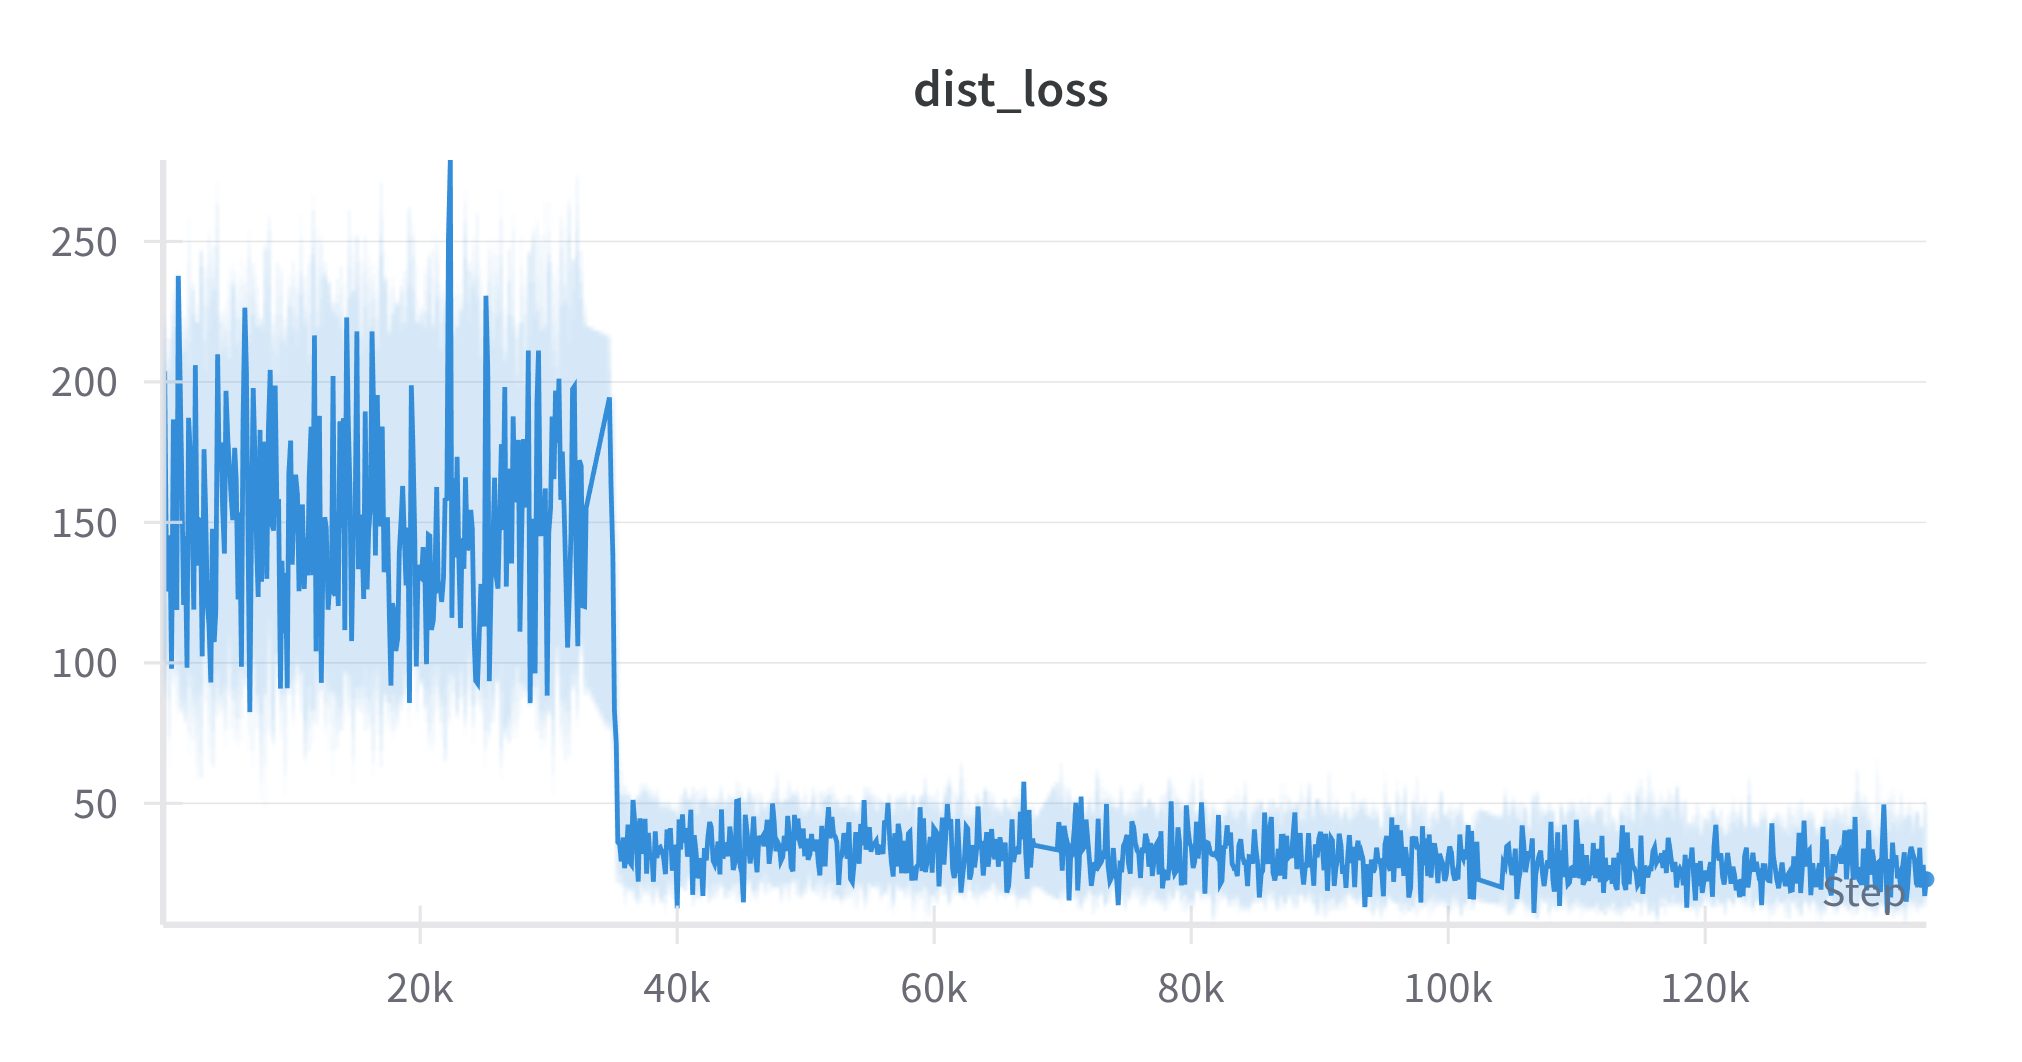
\includegraphics[width=\textwidth]{images/dist_loss.png}
                \textbf{Distance Loss}
            \end{minipage}
            \hfill
            \begin{minipage}{0.48\textwidth}
                \centering
                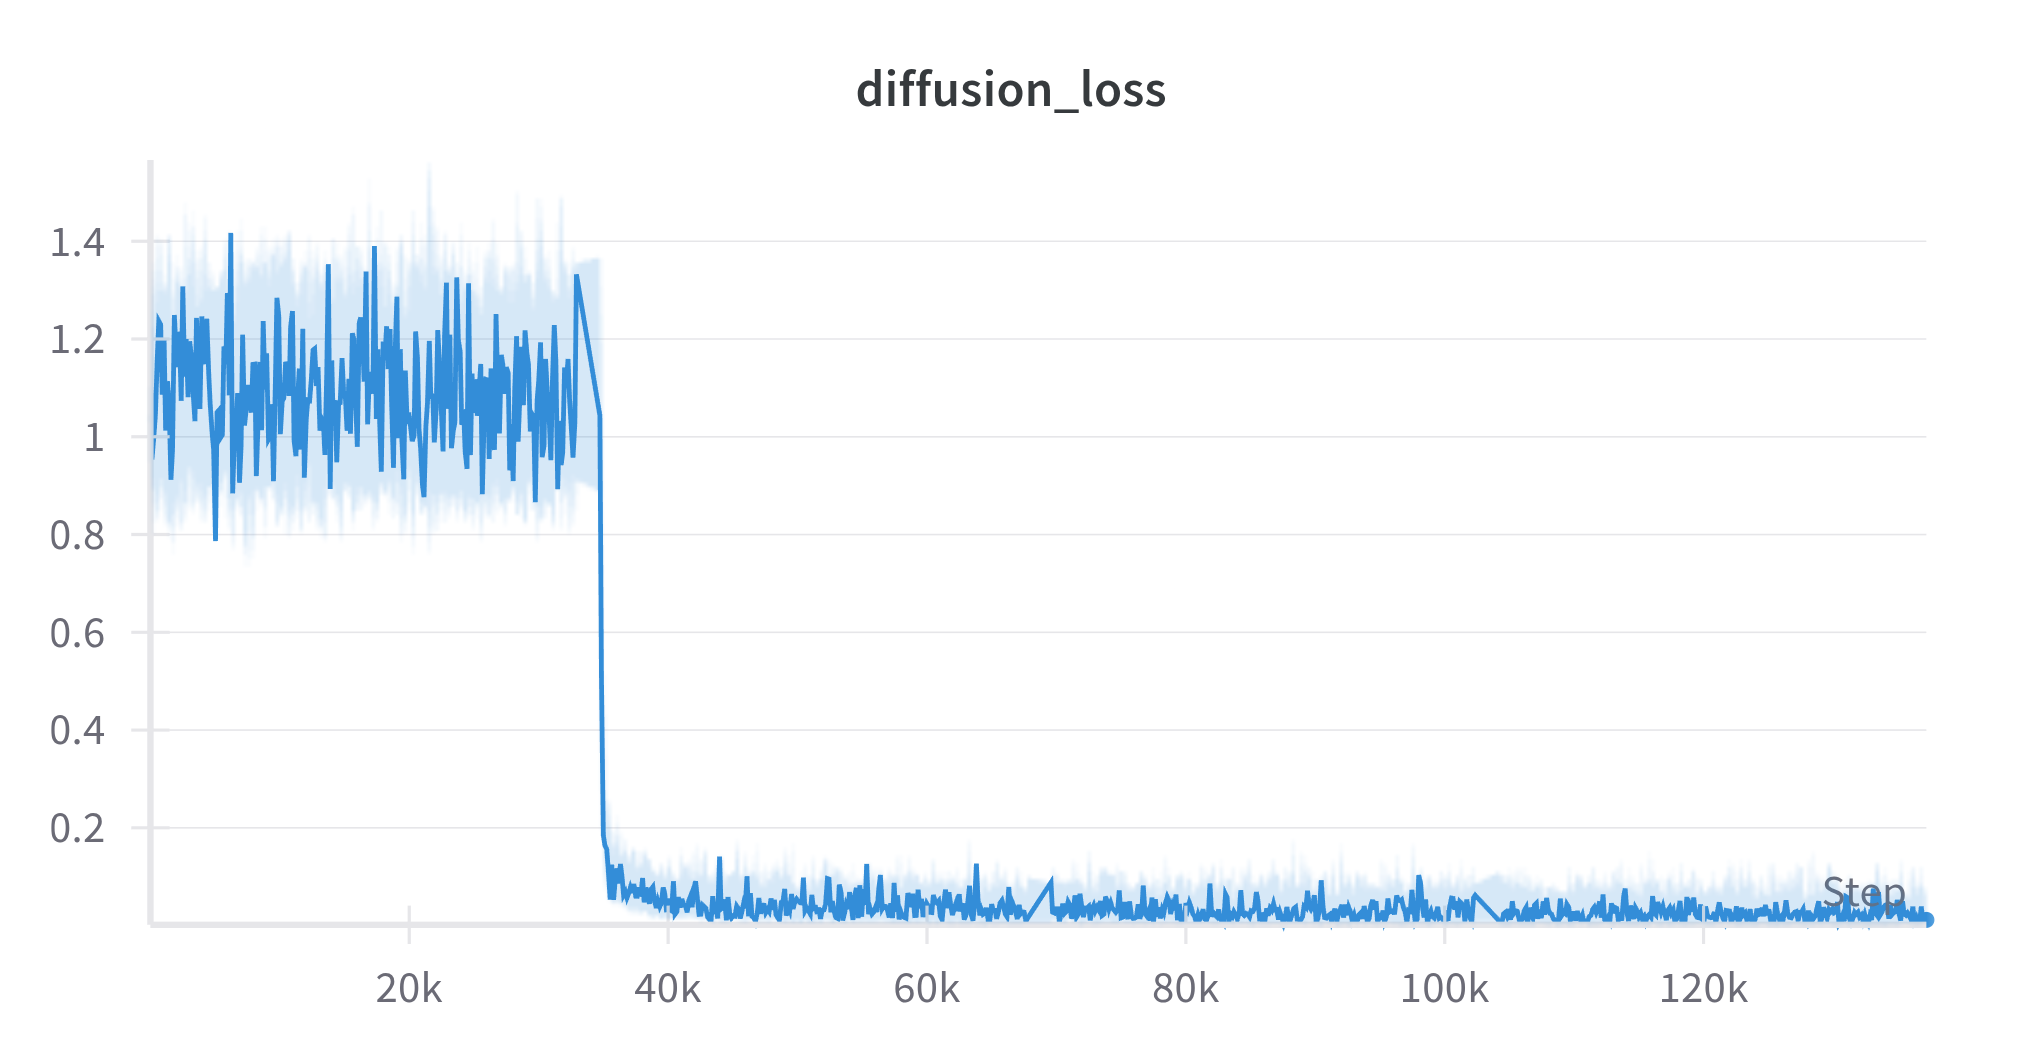
\includegraphics[width=\textwidth]{images/diffusion_loss.png}
                \textbf{Diffusion Loss}
            \end{minipage}
        \end{block}
    The sharp drop in loss around 35k steps marks a point where the model begins to learn more effectively.
    The losses stabilizes at a low value in the later stages, indicating that the model has successfully converged to a well-optimized solution for the training data.
    \end{frame}
    \begin{frame}{Experiments and Results: Diffusion Loss on Validation Set}
        \begin{columns}
            % Goal-Conditioned (m = 0)
            \begin{column}{0.48\textwidth}
                \begin{block}{\centering Goal-Conditioned ($m = 0$)}
                    \centering
                    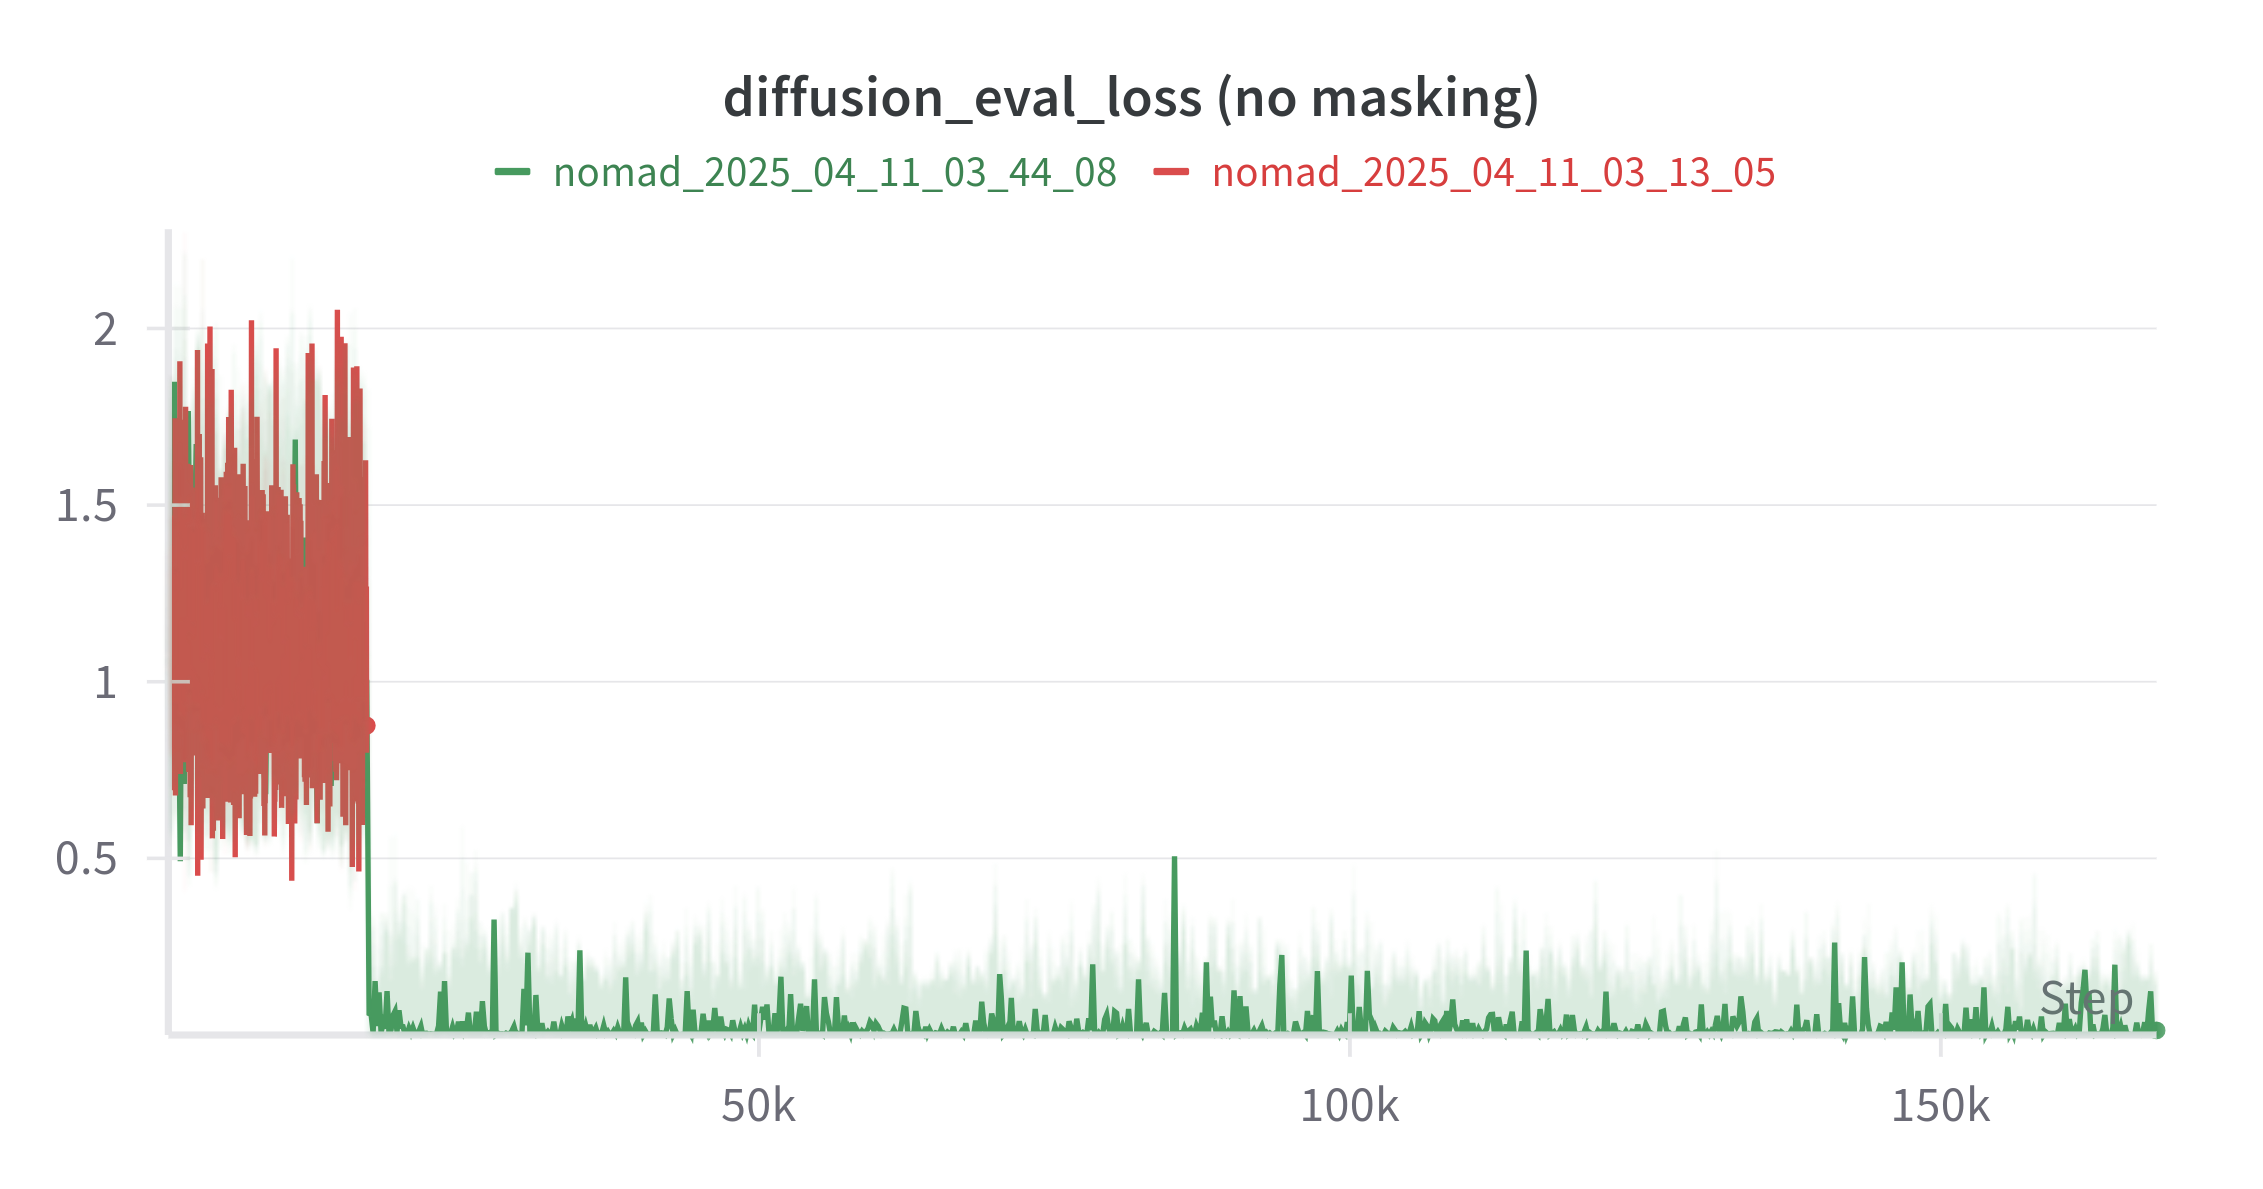
\includegraphics[width=\textwidth]{images/diff_eval_no_masking.png}
                    
                    \vspace{0.5em}
                    \tiny \textbf{All tokens receive goal signal.} \\
                    Evaluates the robot’s ability to follow a target.
                \end{block}
            \end{column}
            
            % Unconditioned (m = 1)
            \begin{column}{0.48\textwidth}
                \begin{block}{\centering Unconditioned ($m = 1$)}
                    \centering
                    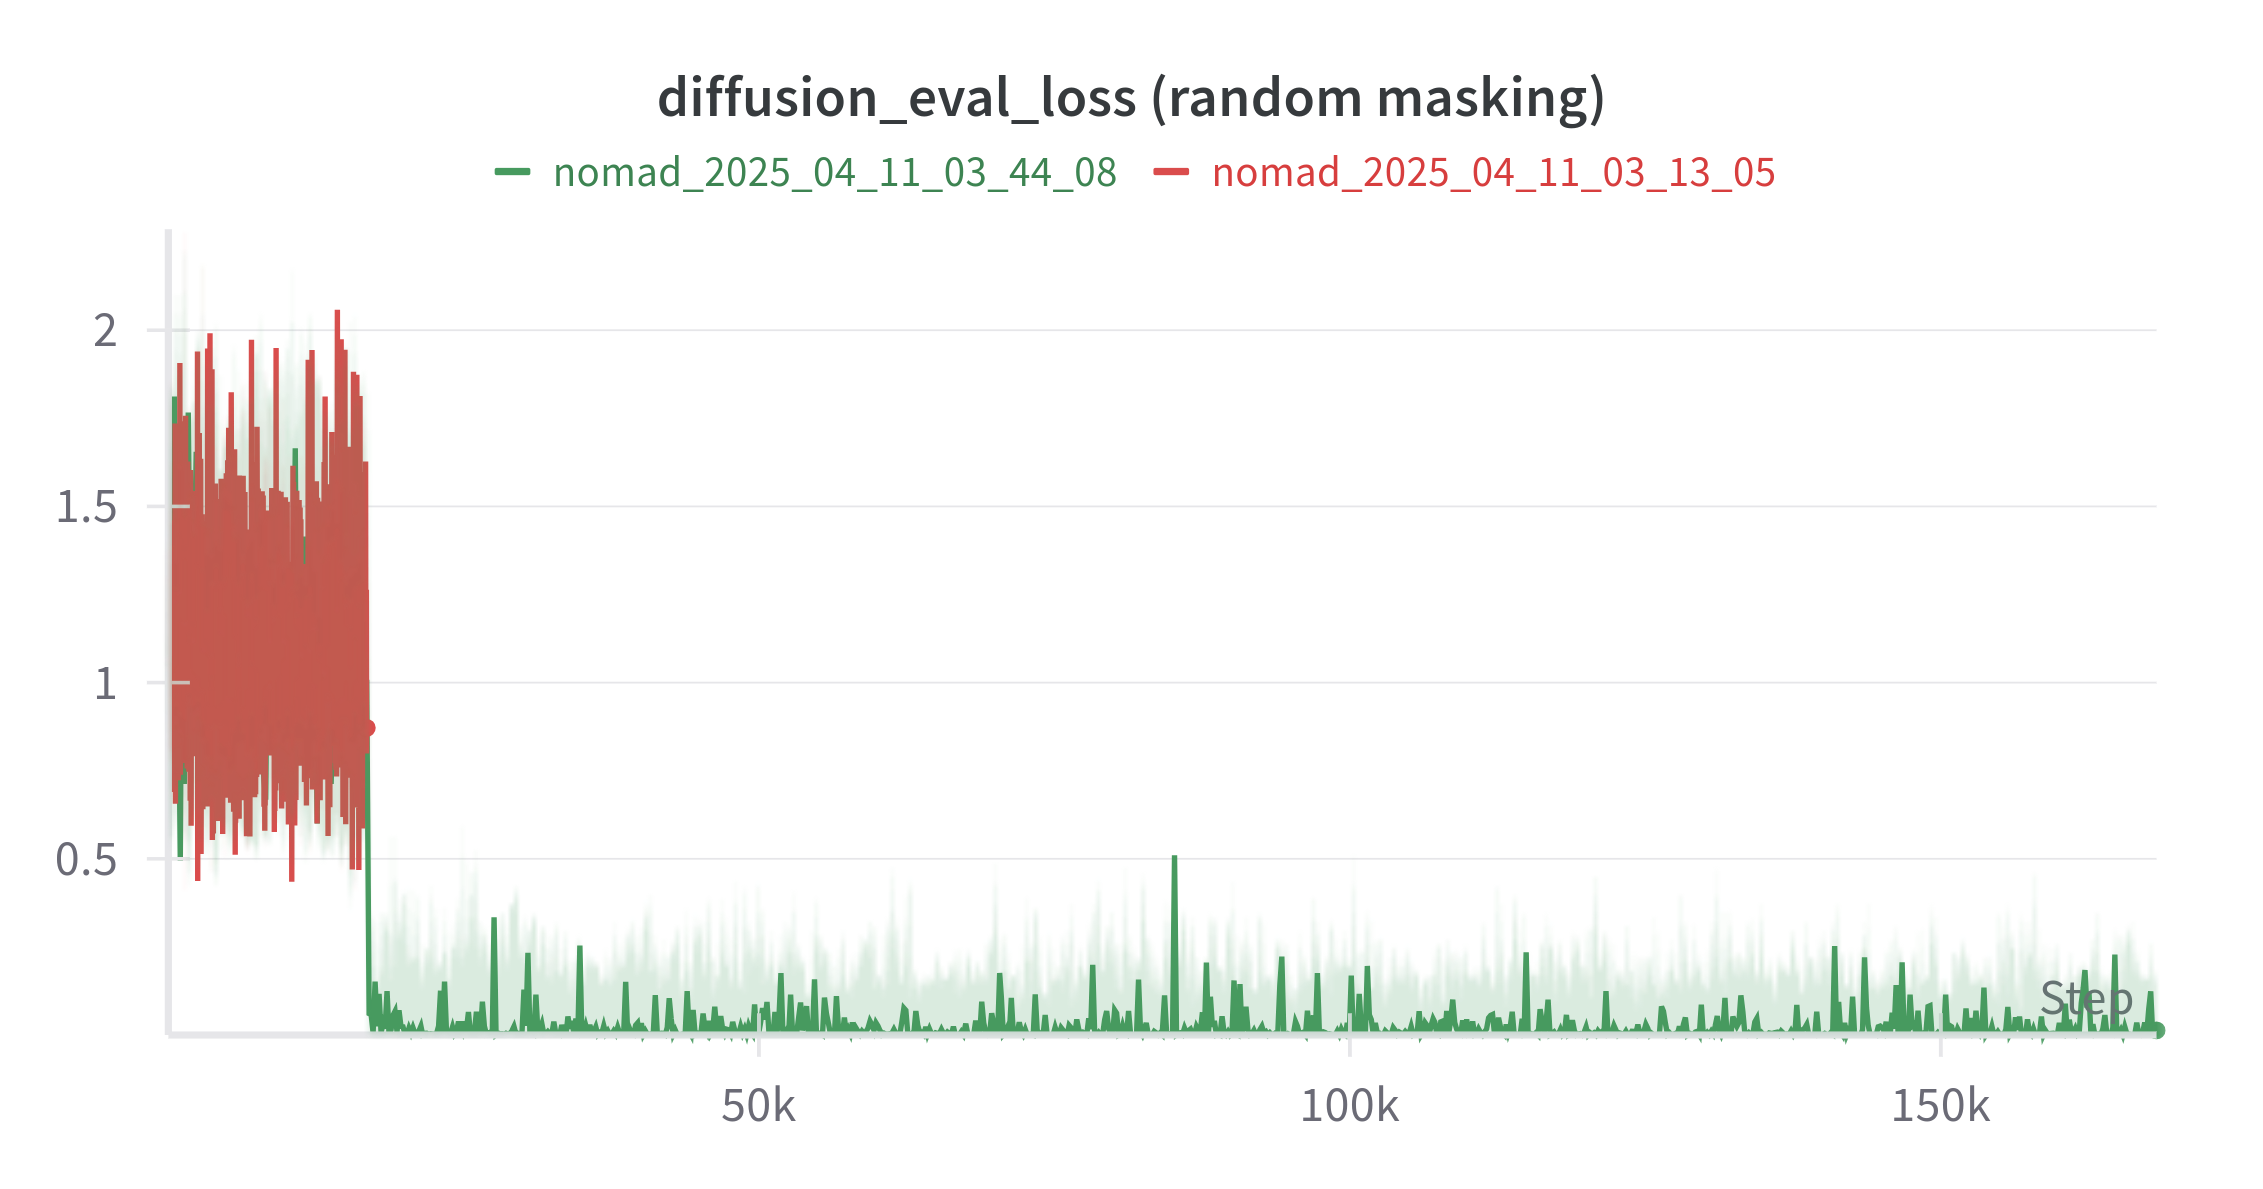
\includegraphics[width=\textwidth]{images/diff_eval_random.png}
                    
                    \vspace{0.5em}
                    \tiny \textbf{No goal information.} \\
                    Evaluates purely exploratory navigation behavior.
                \end{block}
            \end{column}
        \end{columns}
        
        \vspace{0.7em}
        \centering
        \small \textit{We see that loss goes downstream in both cases.}
    \end{frame}

    \begin{frame}{Evaluation: Mixed Masking ( $m \sim \mathcal{B}er(0.5)$ )}
        \begin{block}{Stochastic Goal Conditioning}
            \centering
            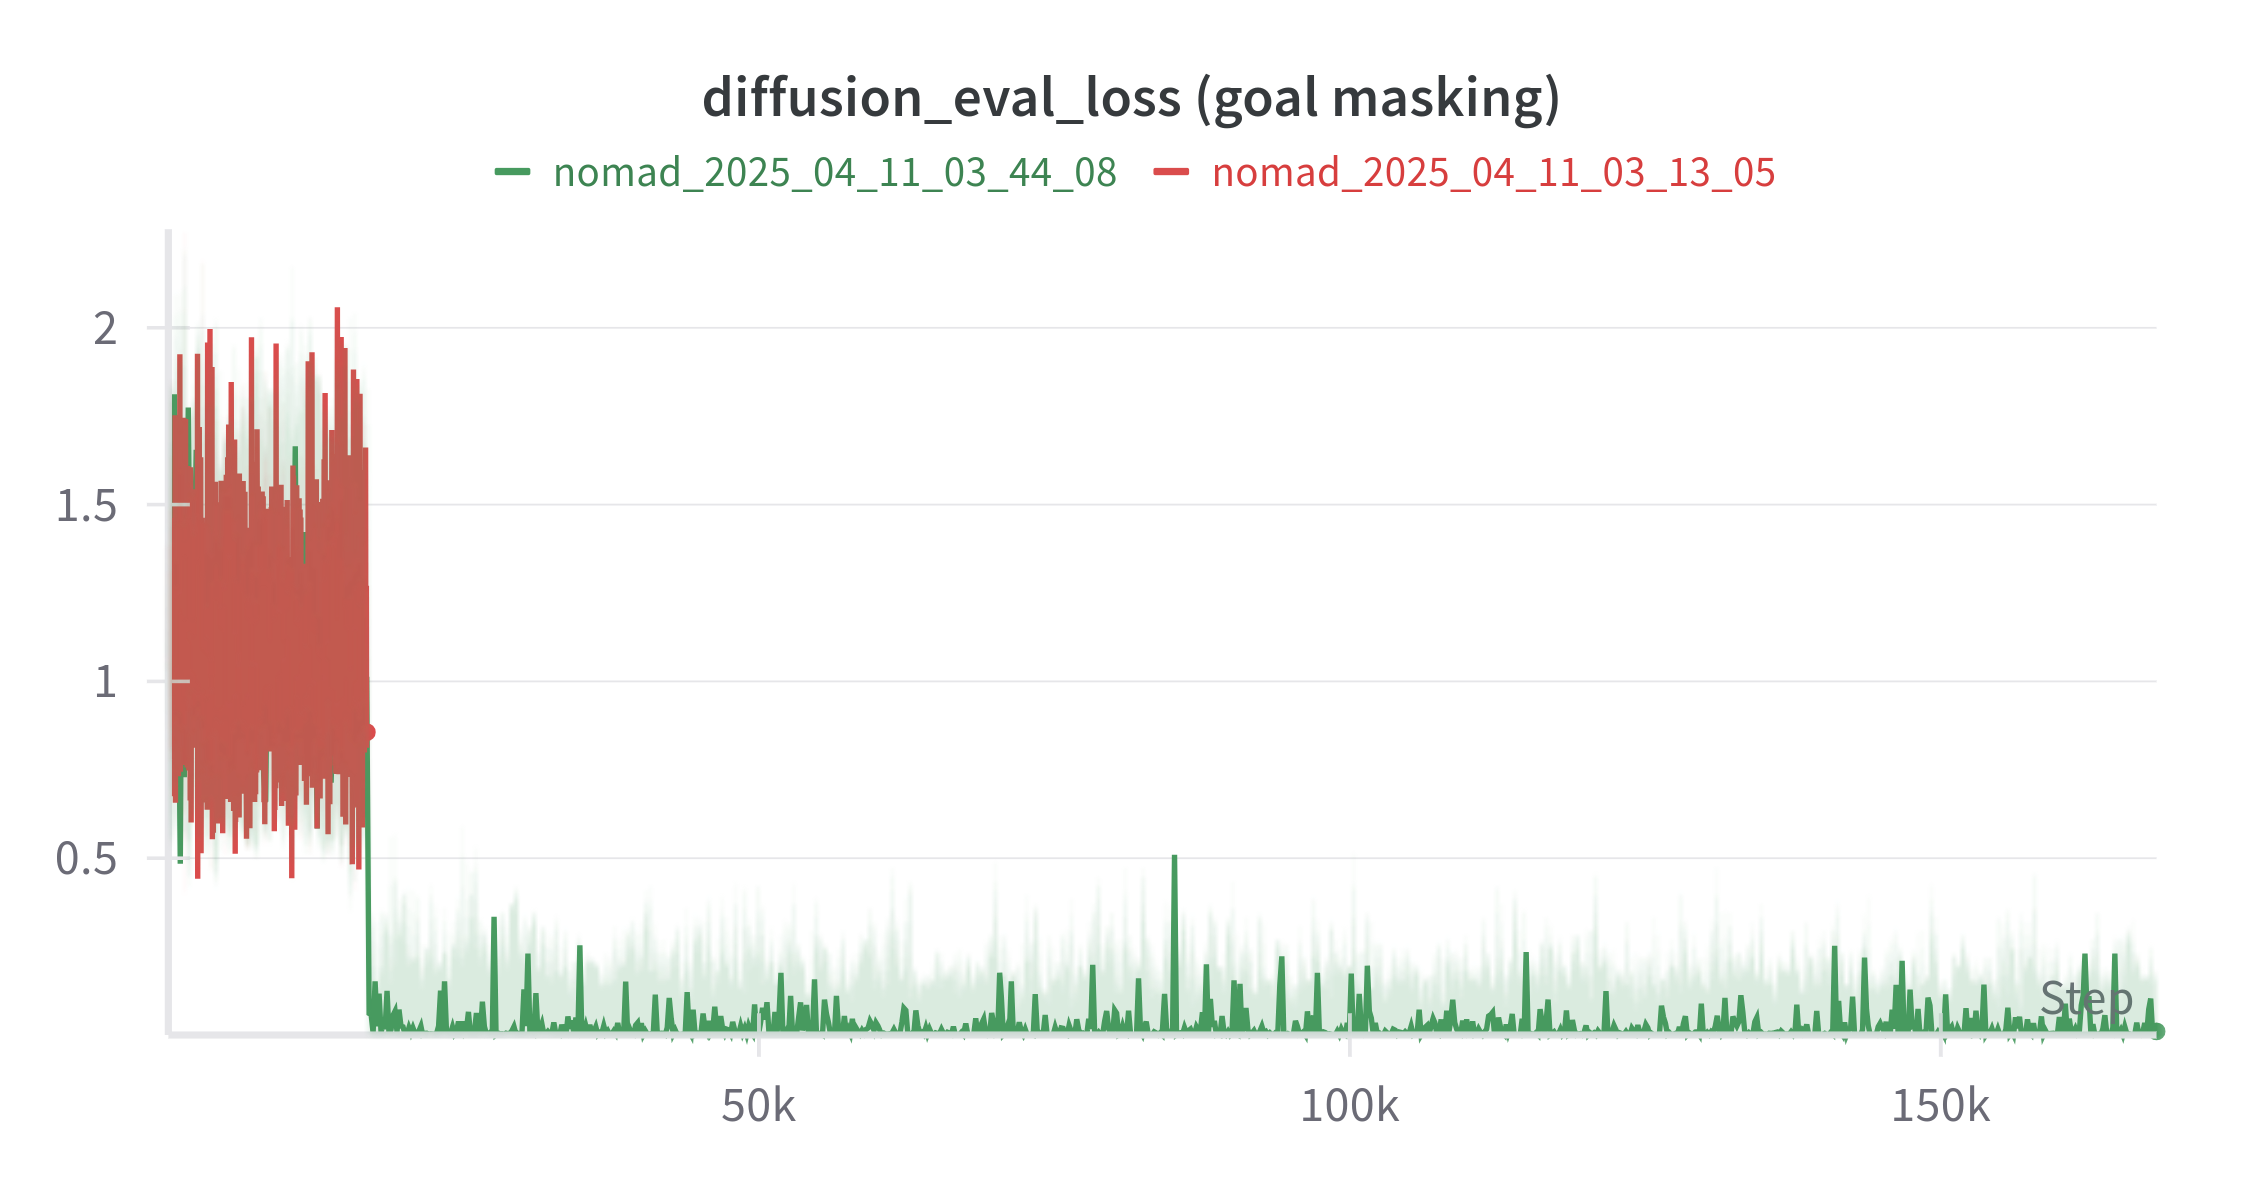
\includegraphics[width=0.8\textwidth]{images/diff_eval_goal_masking.png}
        \end{block}
        \textbf{Description:} \\
        Each token is randomly masked with probability 0.5. This encourages the model to balance between exploring and exploiting goal cues.
    \end{frame}
\begin{frame}{Experiments and Results :Total Loss}
    \begin{block}{Total Loss}
        \centering
        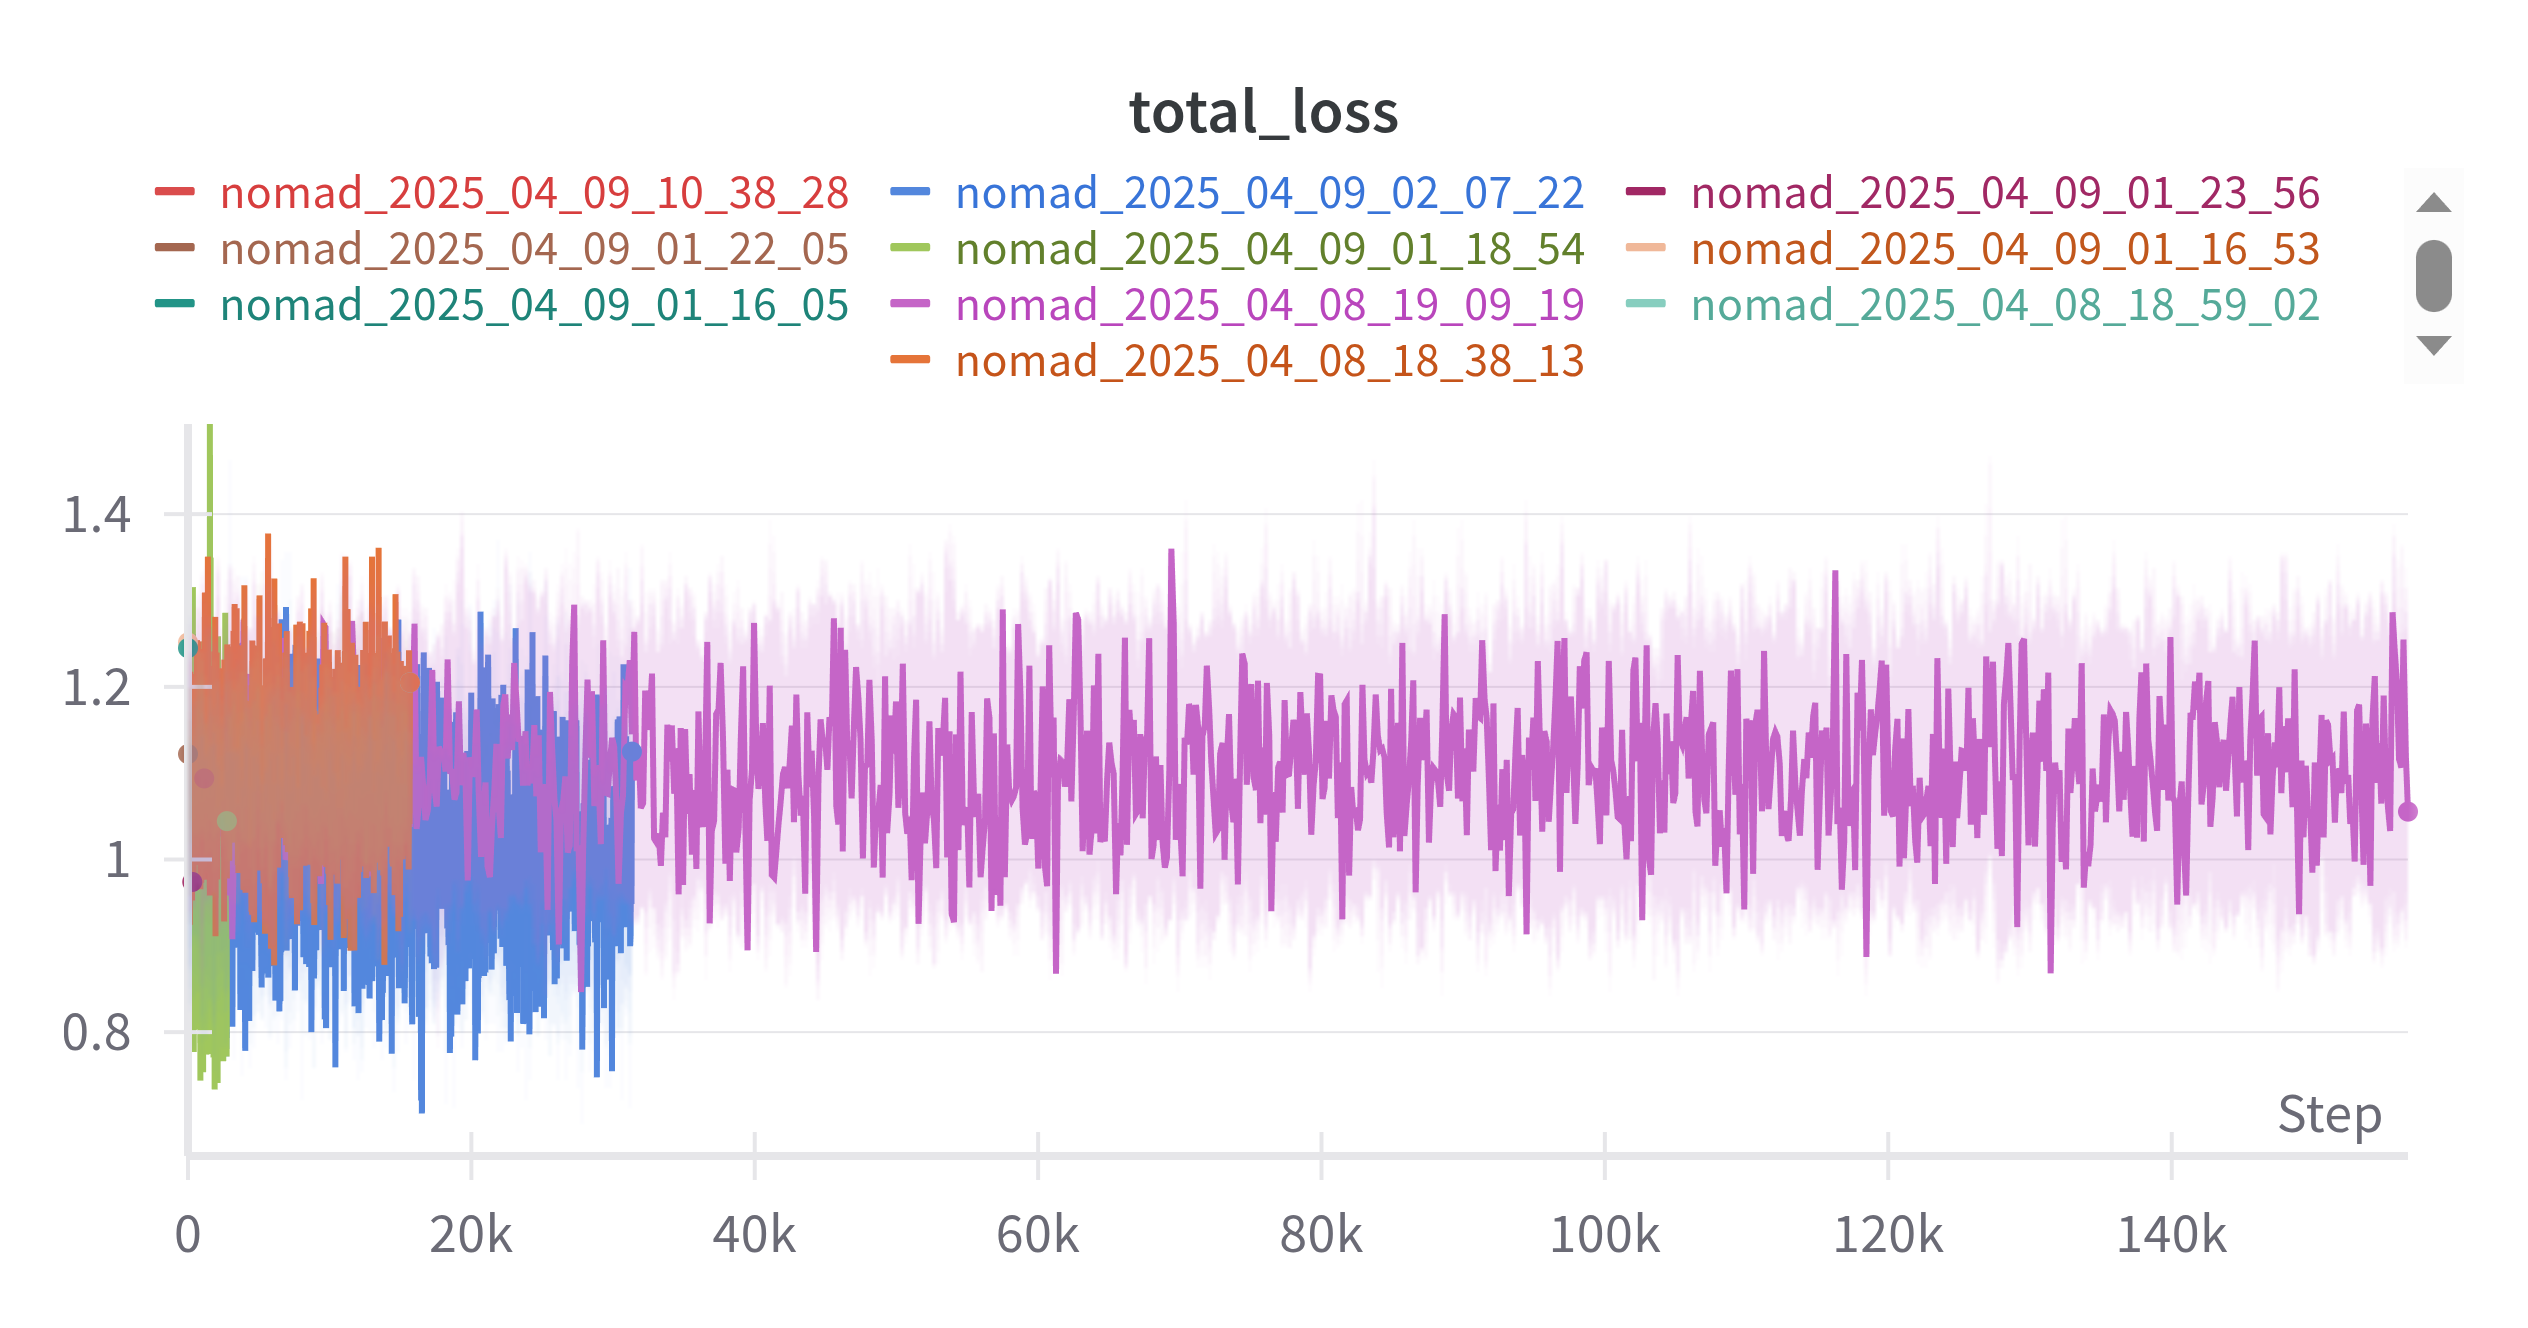
\includegraphics[width=0.75\textwidth]{images/total_loss.png}
        
        \vspace{0.5em}
        \small
        \textbf{Description:} 
        The total loss combines both the diffusion and distance losses, providing a holistic measure of model performance. The model appears to converge to a stable solution.
    \end{block}
\end{frame}


\begin{frame}{Comparision with ViNT: Temporal Distance Loss}
        \begin{block}{Motivation}
            ViNT serves as a strong baseline for visual navigation with transformer-based context encoding. We compare its distance prediction ability against NoMaD.
        \end{block}
    
        \begin{columns}
            \begin{column}{0.48\textwidth}
                \begin{block}{\centering \small \textbf{NoMaD Distance Loss}}
                    \centering
                    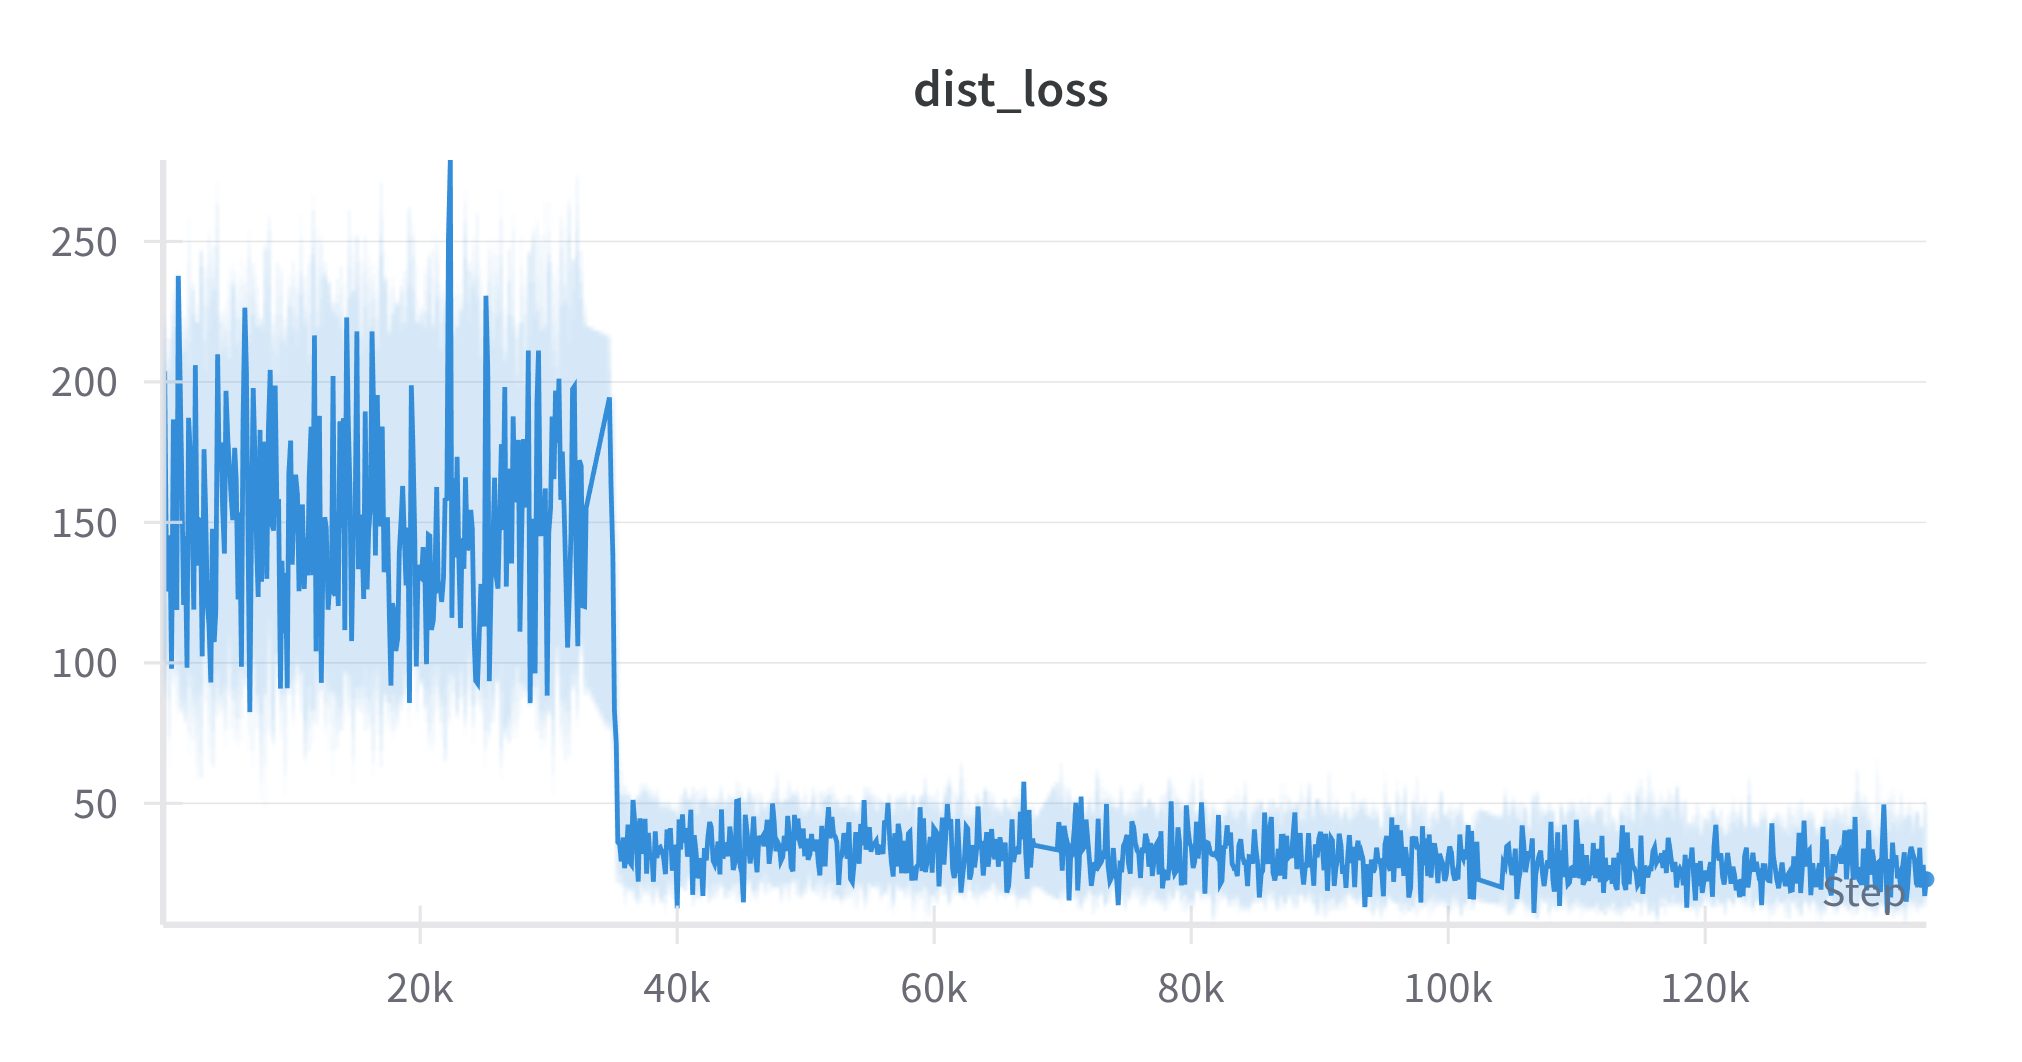
\includegraphics[width=\textwidth]{images/dist_loss.png}
                    \tiny NoMaD achieves lower and more stable distance loss due to diffusion-based modeling and goal conditioning.
                \end{block}
            \end{column}
    
            \begin{column}{0.48\textwidth}
                \begin{block}{\centering \small \textbf{ViNT Distance Loss}}
                    \centering
                    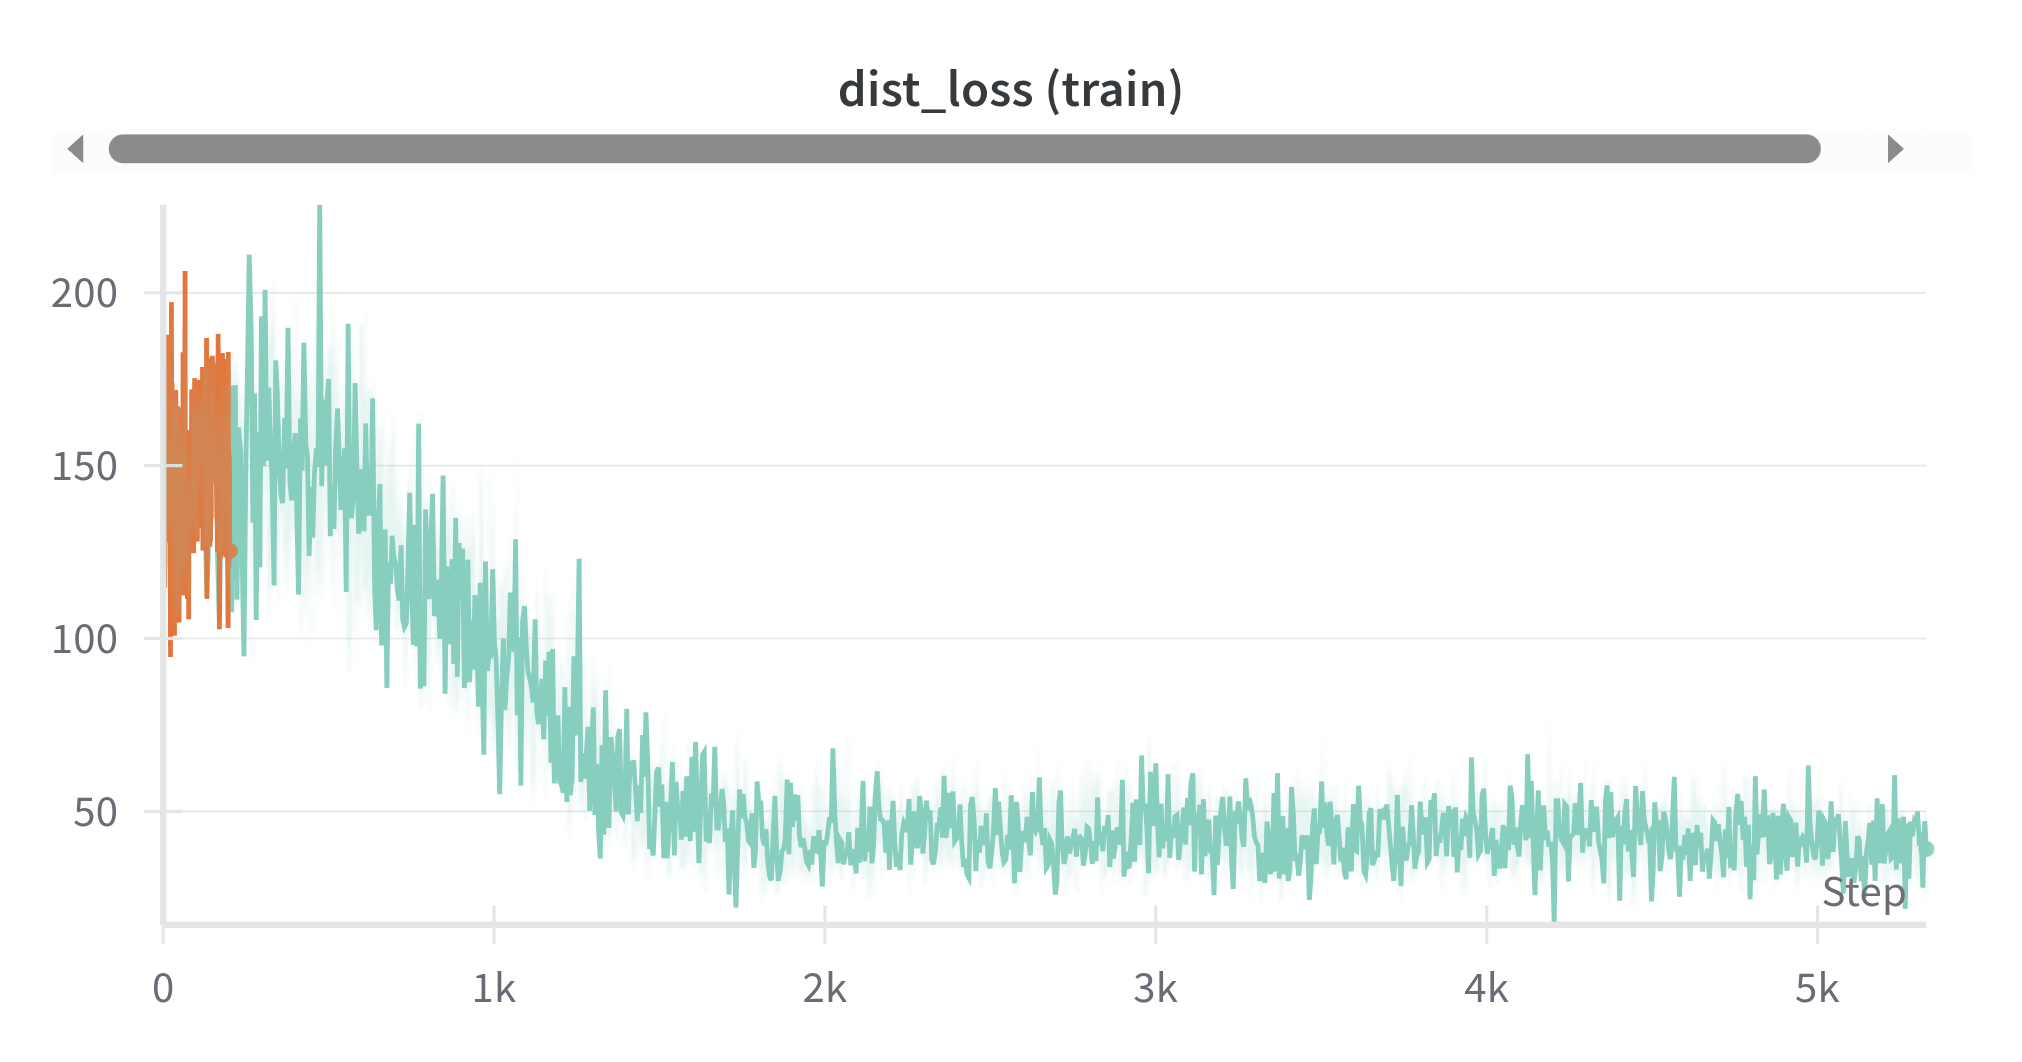
\includegraphics[width=\textwidth]{images/dist_loss (train).png}
                    \tiny ViNT performs comparably in early epochs but struggles with long-horizon distance regression.
                \end{block}
            \end{column}
        \end{columns}
    
        \vspace{0.5em}
        \centering
        \textit{Observation:} \textbf{NoMaD’s diffusion-based decoder improves distance supervision} without sacrificing ViNT’s transformer strengths.
\end{frame}

\begin{frame}{ViNT vs NoMaD: Action Loss}
    \begin{block}{Objective}
        We compare the quality of predicted waypoints by measuring the Mean Squared Error (MSE) between predicted and ground-truth actions.
    \end{block}

    \begin{columns}
        \begin{column}{0.48\textwidth}
            \begin{block}{\centering \small \textbf{NoMaD Action Loss}}
                \centering
                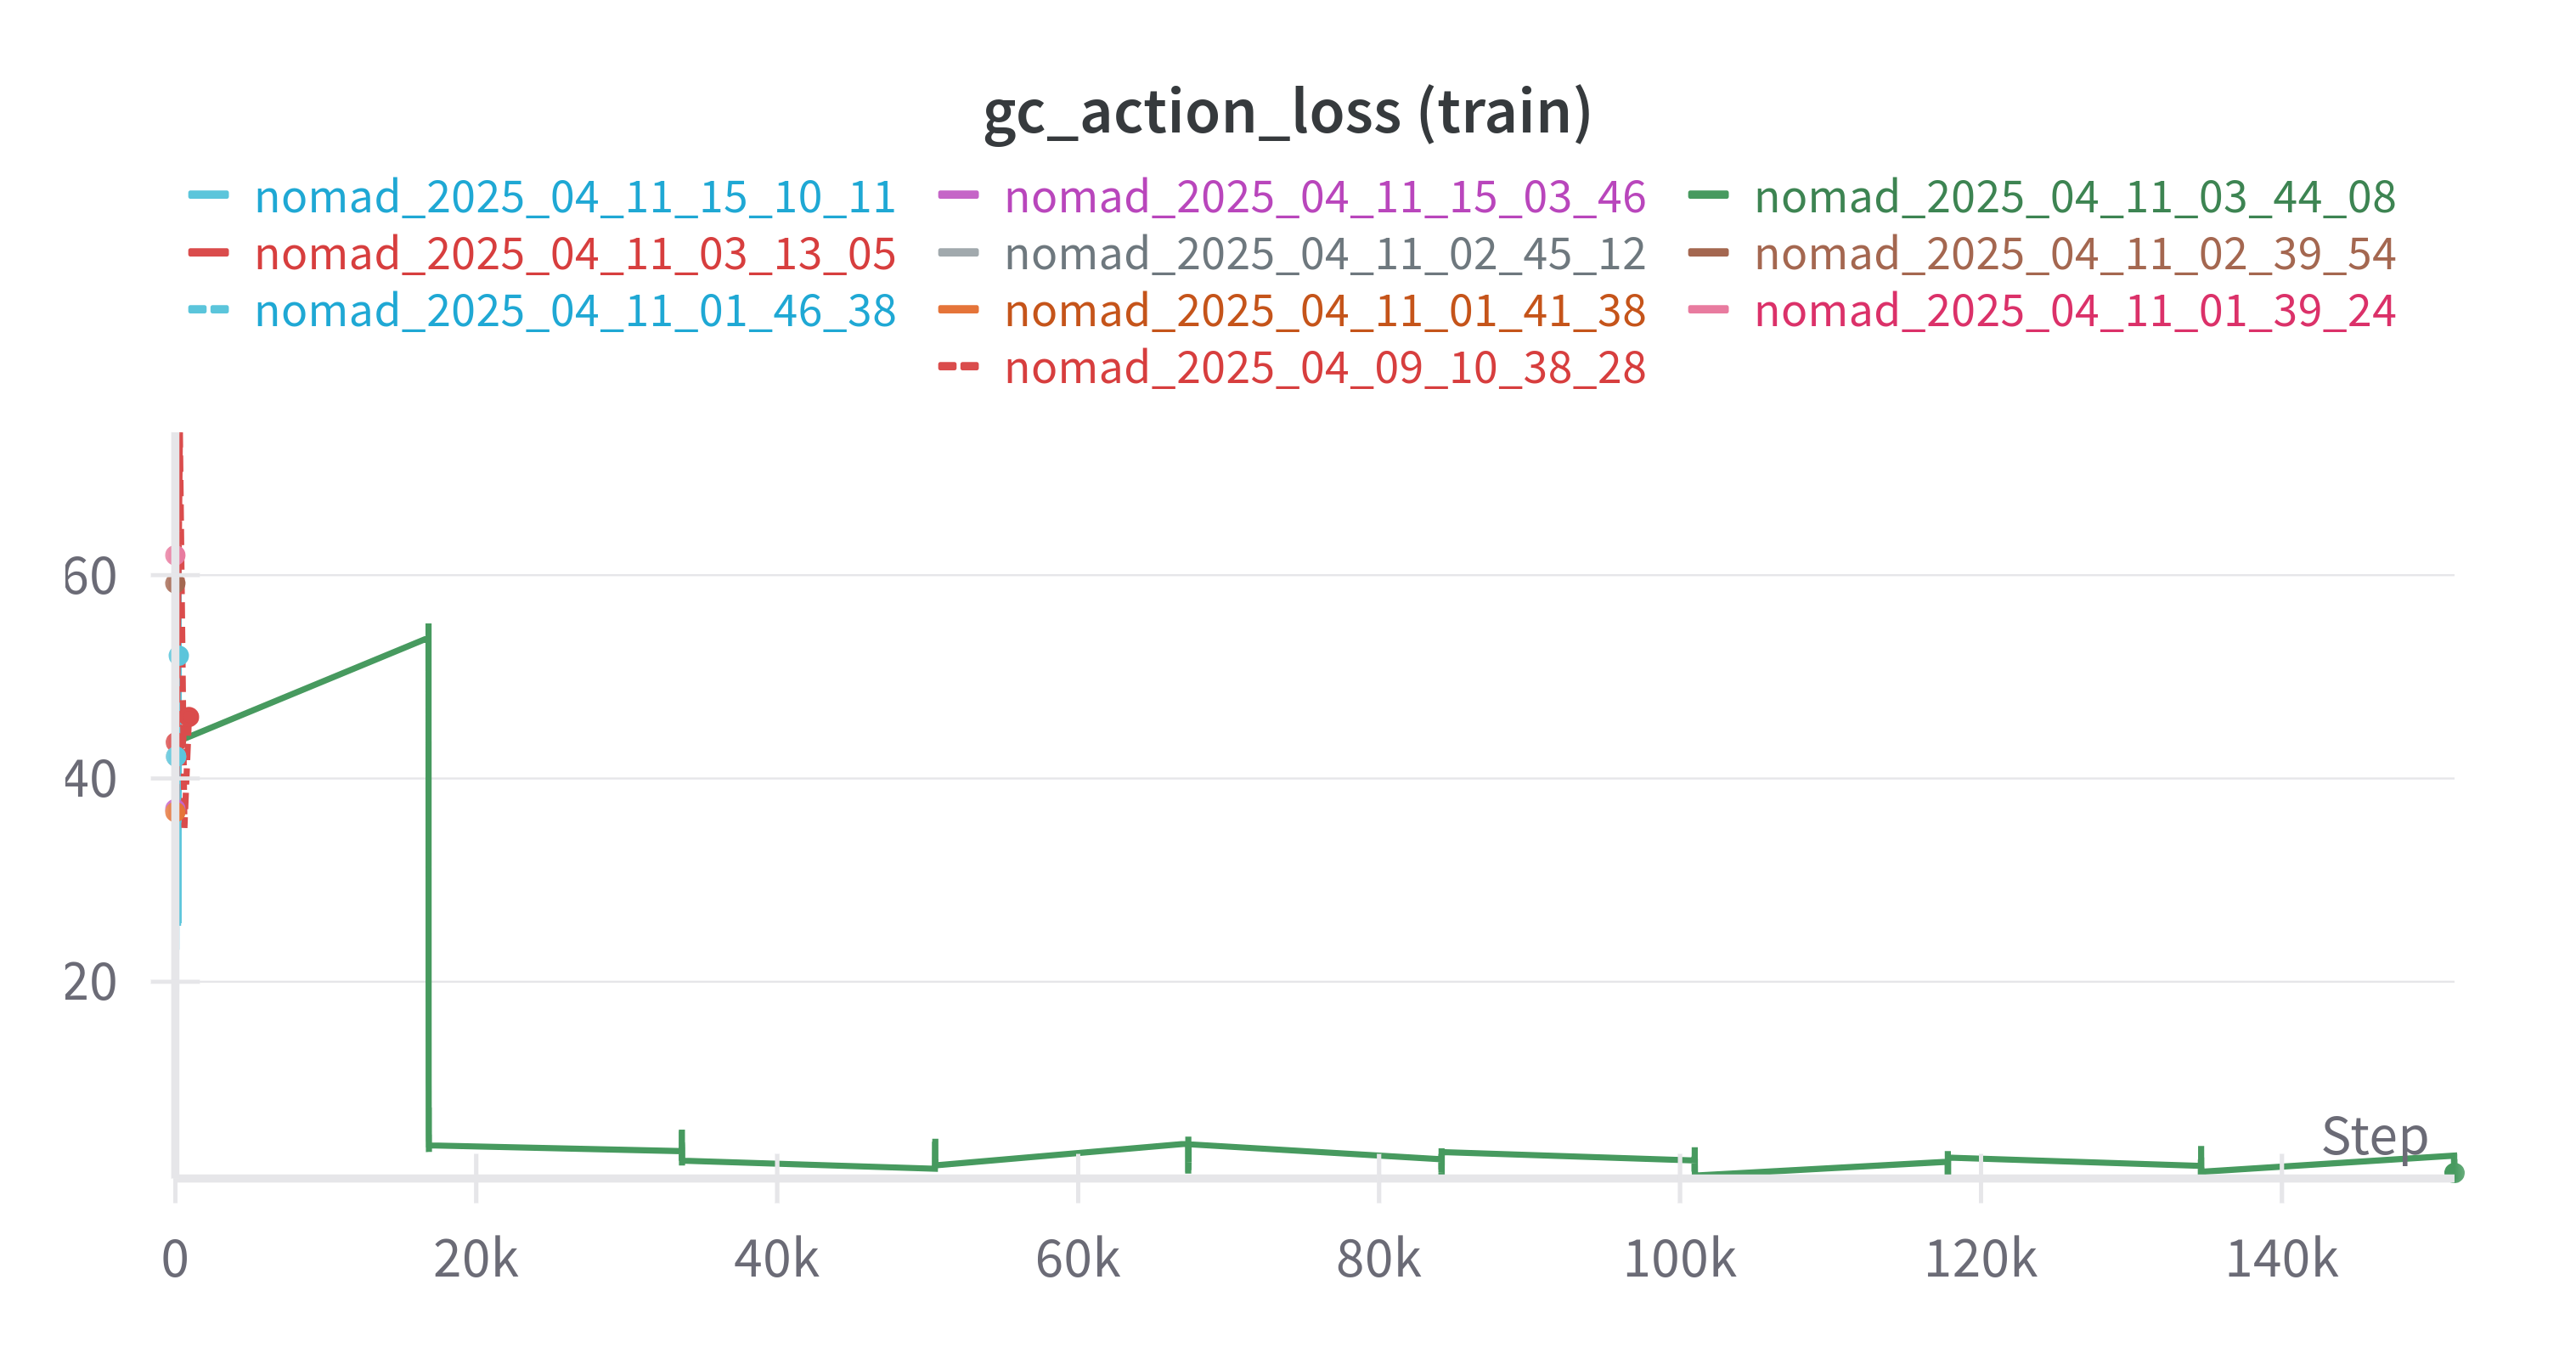
\includegraphics[width=\textwidth]{images/gc_actionloss_nomad.png}
                \tiny NoMaD consistently achieves lower action loss, aided by the stochastic denoising process and goal-conditioned context.
            \end{block}
        \end{column}

        \begin{column}{0.48\textwidth}
            \begin{block}{\centering \small \textbf{ViNT Action Loss}}
                \centering
                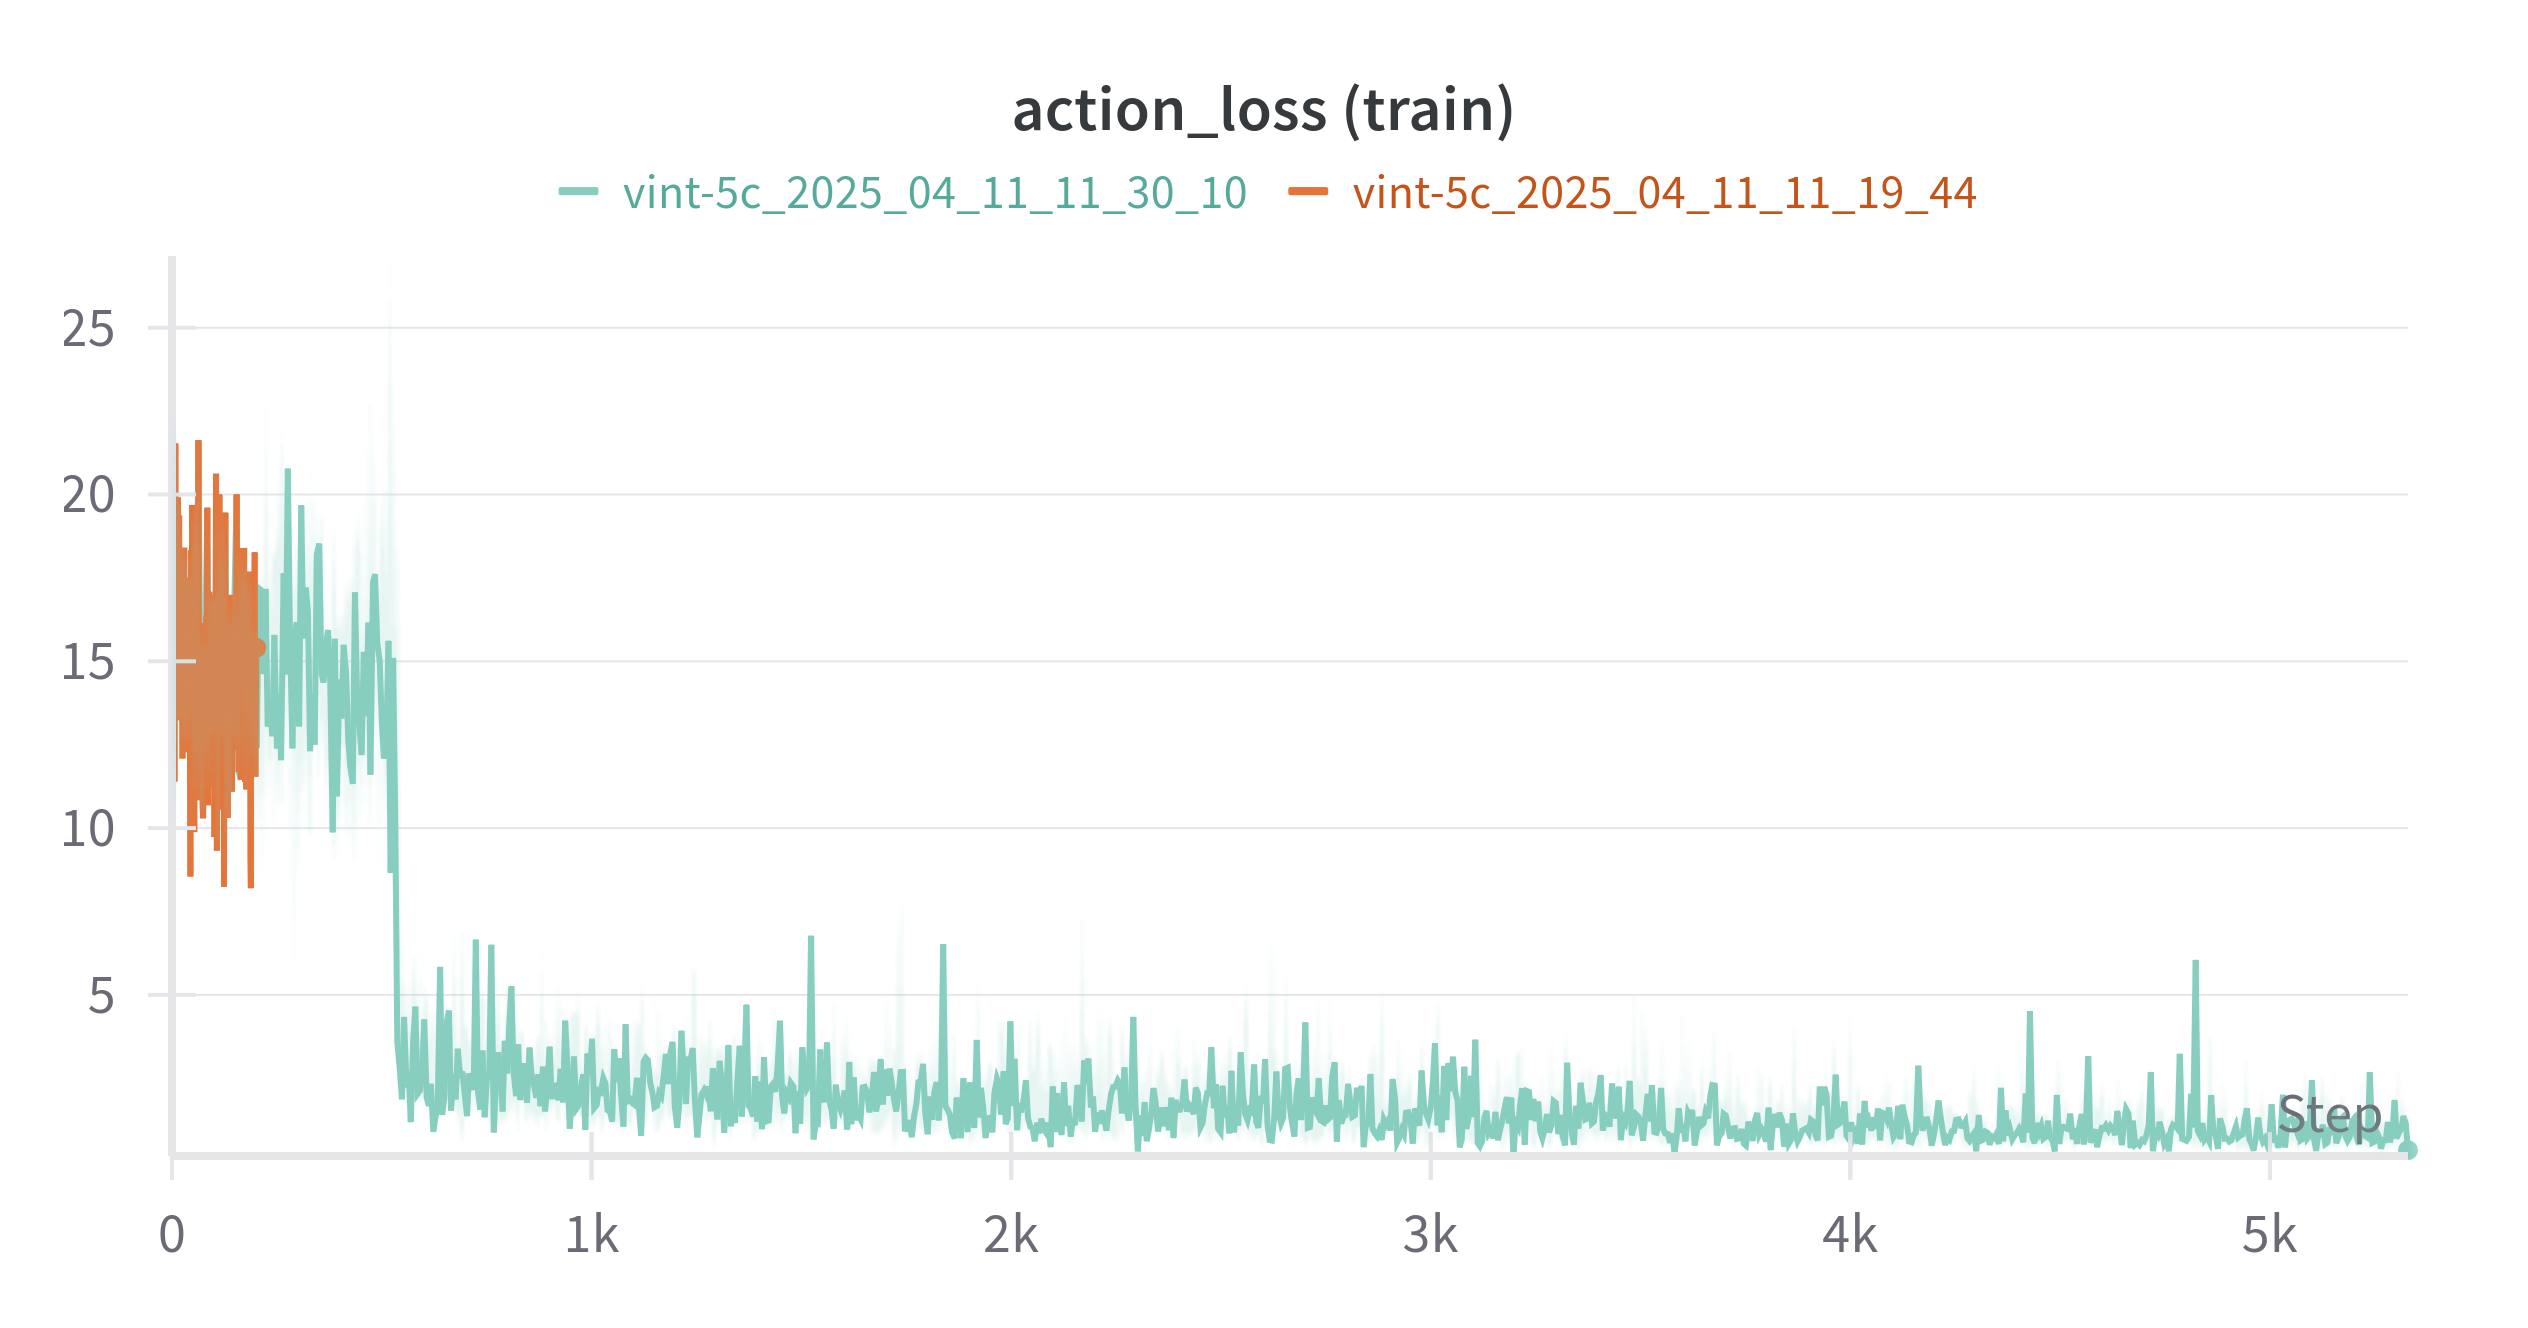
\includegraphics[width=\textwidth]{images/action_train_vint.png}
                \tiny ViNT shows slightly higher variance, and loss plateaus earlier due to MLP-based decoding.
            \end{block}
        \end{column}
    \end{columns}

    \vspace{0.5em}
    \centering
    \textit{Observation:} \textbf{NoMaD benefits from the expressiveness of diffusion decoding} in predicting fine-grained waypoint actions.
\end{frame}

\begin{frame}{Comparison with ViNT: Total Loss}
    \begin{block}{Motivation}
        To assess the overall effectiveness of NoMaD vs. ViNT, we compare the combined loss: action prediction loss + temporal distance prediction loss.
    \end{block}

    \begin{columns}
        \begin{column}{0.48\textwidth}
            \begin{block}{\centering \small \textbf{NoMaD Total Loss}}
                \centering
                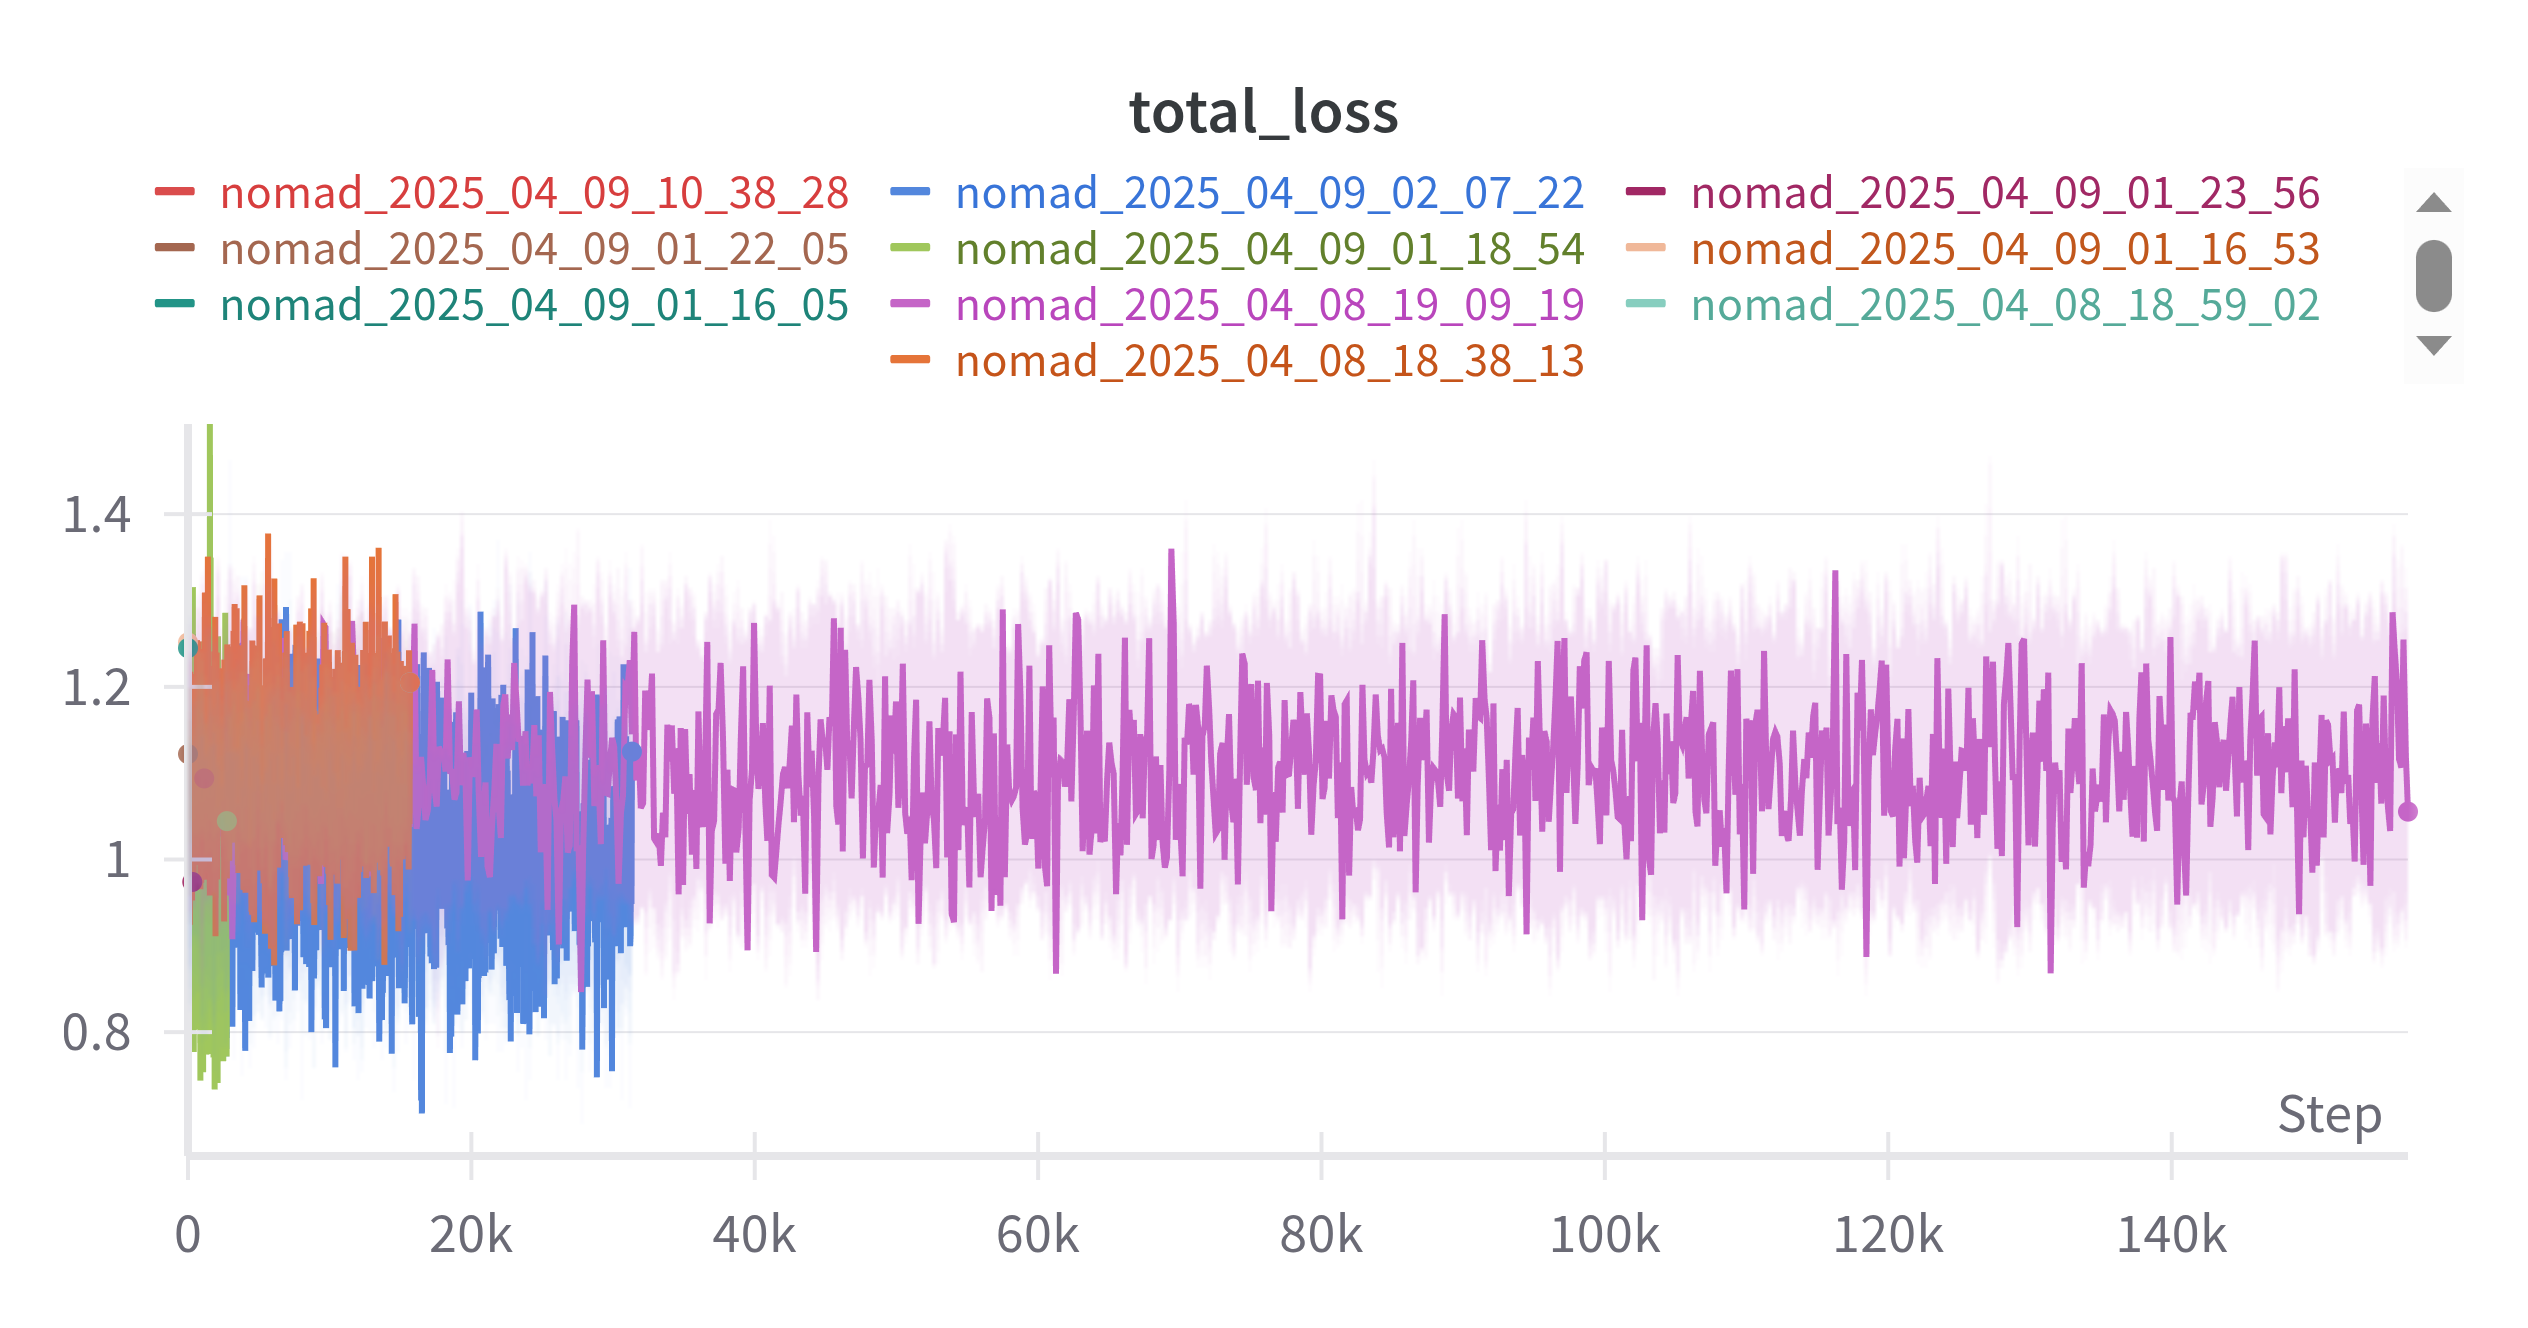
\includegraphics[width=\textwidth]{images/total_loss.png}
                \tiny NoMaD achieves better convergence, with lower final loss due to richer diffusion-based decoding.
            \end{block}
        \end{column}

        \begin{column}{0.48\textwidth}
            \begin{block}{\centering \small \textbf{ViNT Total Loss}}
                \centering
                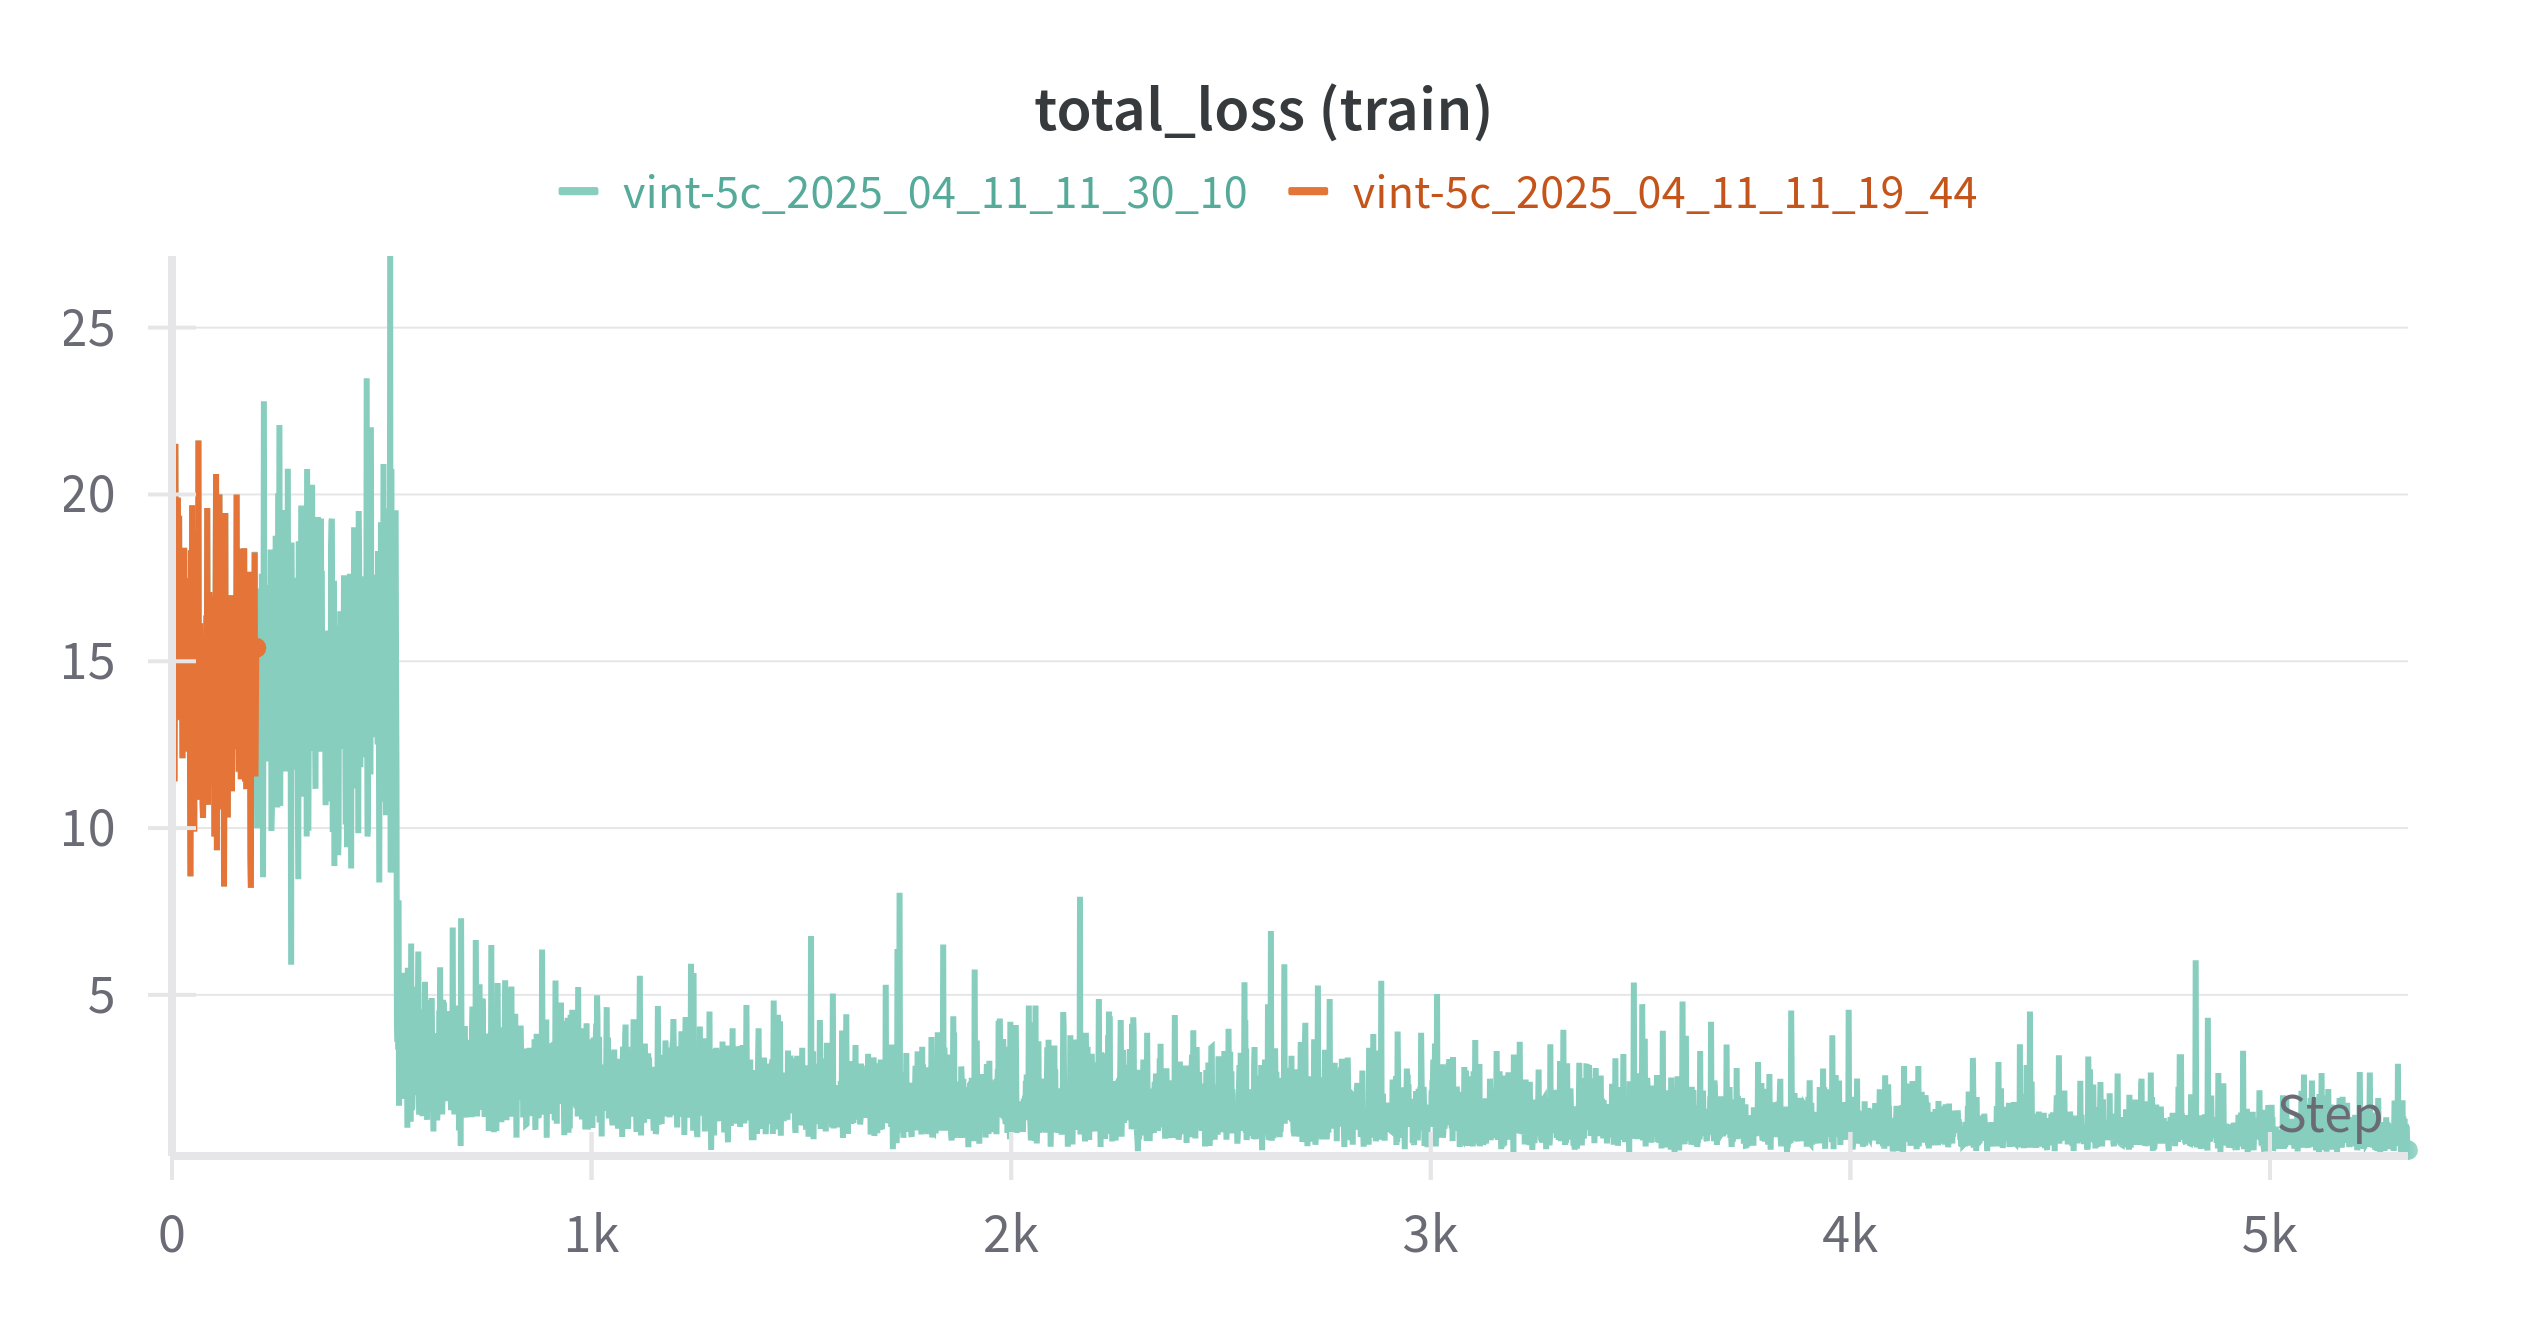
\includegraphics[width=\textwidth]{images/distloss_vint.png}
                \tiny ViNT exhibits slower learning and higher loss, limited by direct MLP-based action prediction.
            \end{block}
        \end{column}
    \end{columns}

    \vspace{0.5em}
    \centering
    \textit{Takeaway:} \textbf{NoMaD demonstrates improved learning dynamics and generalization.}
\end{frame}

\begin{frame}{Challenges Faced}
    \begin{itemize}
        \item CUDA out of memory errors were common during training, especially with larger batch sizes. We mitigated this by reducing the batch size and using gradient accumulation.
        \item The model was initially not being able to learn effectively, leading to high loss values. We debugged this by checking the data pipeline and ensuring that the input images were correctly preprocessed and normalized.
        \item The system in UG computational labs didnot have ROS installed, which was required to process the datasets. With the help of our TA, we used a docker file to set up a container with ROS and the required dependencies.
        \item The original codebase has several data-type related bugs which had to be fixed. For example, the original code was using torch.float32 for some tensors, while the model expected them to be in torch.float64. This caused several errors during training.
        \item The initial implementation caused several system crashes due to heavy computational load.
    \end{itemize}
\end{frame}

\begin{frame}{Team Contributions}
    \textbf{Abhishek Kumar Jha:} \\
    \begin{itemize}
        \item Implemented the Nomad Architecture and helped in the Training and Experiments
        \item Made the README file for the repository.
        \item Assisted in creating the report and Presentation.
        \item Contributed towards making the code demo video.
        \item Helped in integrating and debugging the diffusion policy repository
    
    \end{itemize}
    \textbf{Namashivayaa V:} \\
    \begin{itemize}
        \item Explained the workflow of the suggested papers to the entire team.
        \item Contributed in report formation, by adding important formulas and results in the
        appendix section.
        \item Extracted the .bag files which were around 300GB.
    \end{itemize}
\end{frame}

\newpage

\begin{frame}{Team Contributions}
    \textbf{Sehaj Ganjoo:} \\
    \begin{itemize}
        \item Implemented the ViNT architecture and trained it
        \item Helped in debuggeding the errors while training the NoMaD model
        \item Assisted in conducting experiments and analysis for the project
        \item Contributed towards the Presentation and project report
    \end{itemize}
    \textbf{Shobhnik Kriplani:} \\
    \begin{itemize}
        \item Implemented the NoMaD architecture
        \item Developed the training pipeline
        \item Conducted experiments and analysis
        \item Made a website for the project

        
    \end{itemize}
\end{frame}

\begin{frame}{Conclusion and Future Work}
\begin{itemize}
    \item Successfully trained NoMaD using diffusion for visual navigation
    \item Showed compatibility with ViNT-based perception
    \item Future work:
    \begin{itemize}
        \item Deploy NoMaD on real robots and check performance on real world environments
        \item Explore the use of NoMaD for other tasks like object detection and tracking
        \item Explore how we can improve the current architecture.
        \item Try larger ViTs and alternate decoders
    \end{itemize}
\end{itemize}
\end{frame}

\begin{frame}{Q\&A}
    \begin{center}
        \Huge{\textbf{Thank You!}}\\
    \end{center}
\end{frame}

\section{Appendices}
\begin{frame}{Appendices}
    \begin{block}{Appendices}
        \begin{itemize}
            \item Appendix A: Additional Results
            \item Appendix B: Implementation Details
            \item Appendix C: References
        \end{itemize}
    \end{block}
\end{frame}
\begin{frame}{Appendix A: Additional Results}
    \begin{block}{Additional Results}
        \begin{itemize}
            \item Additional results and analysis of NoMaD's performance
        \end{itemize}
    \end{block}
\end{frame}
\begin{frame}{Experiments and Results: Cosine Similarity}
    \begin{block}{Goal-Conditioned Action Waypoints Cosine Similarity}
        \begin{minipage}{0.48\textwidth}
            \centering
            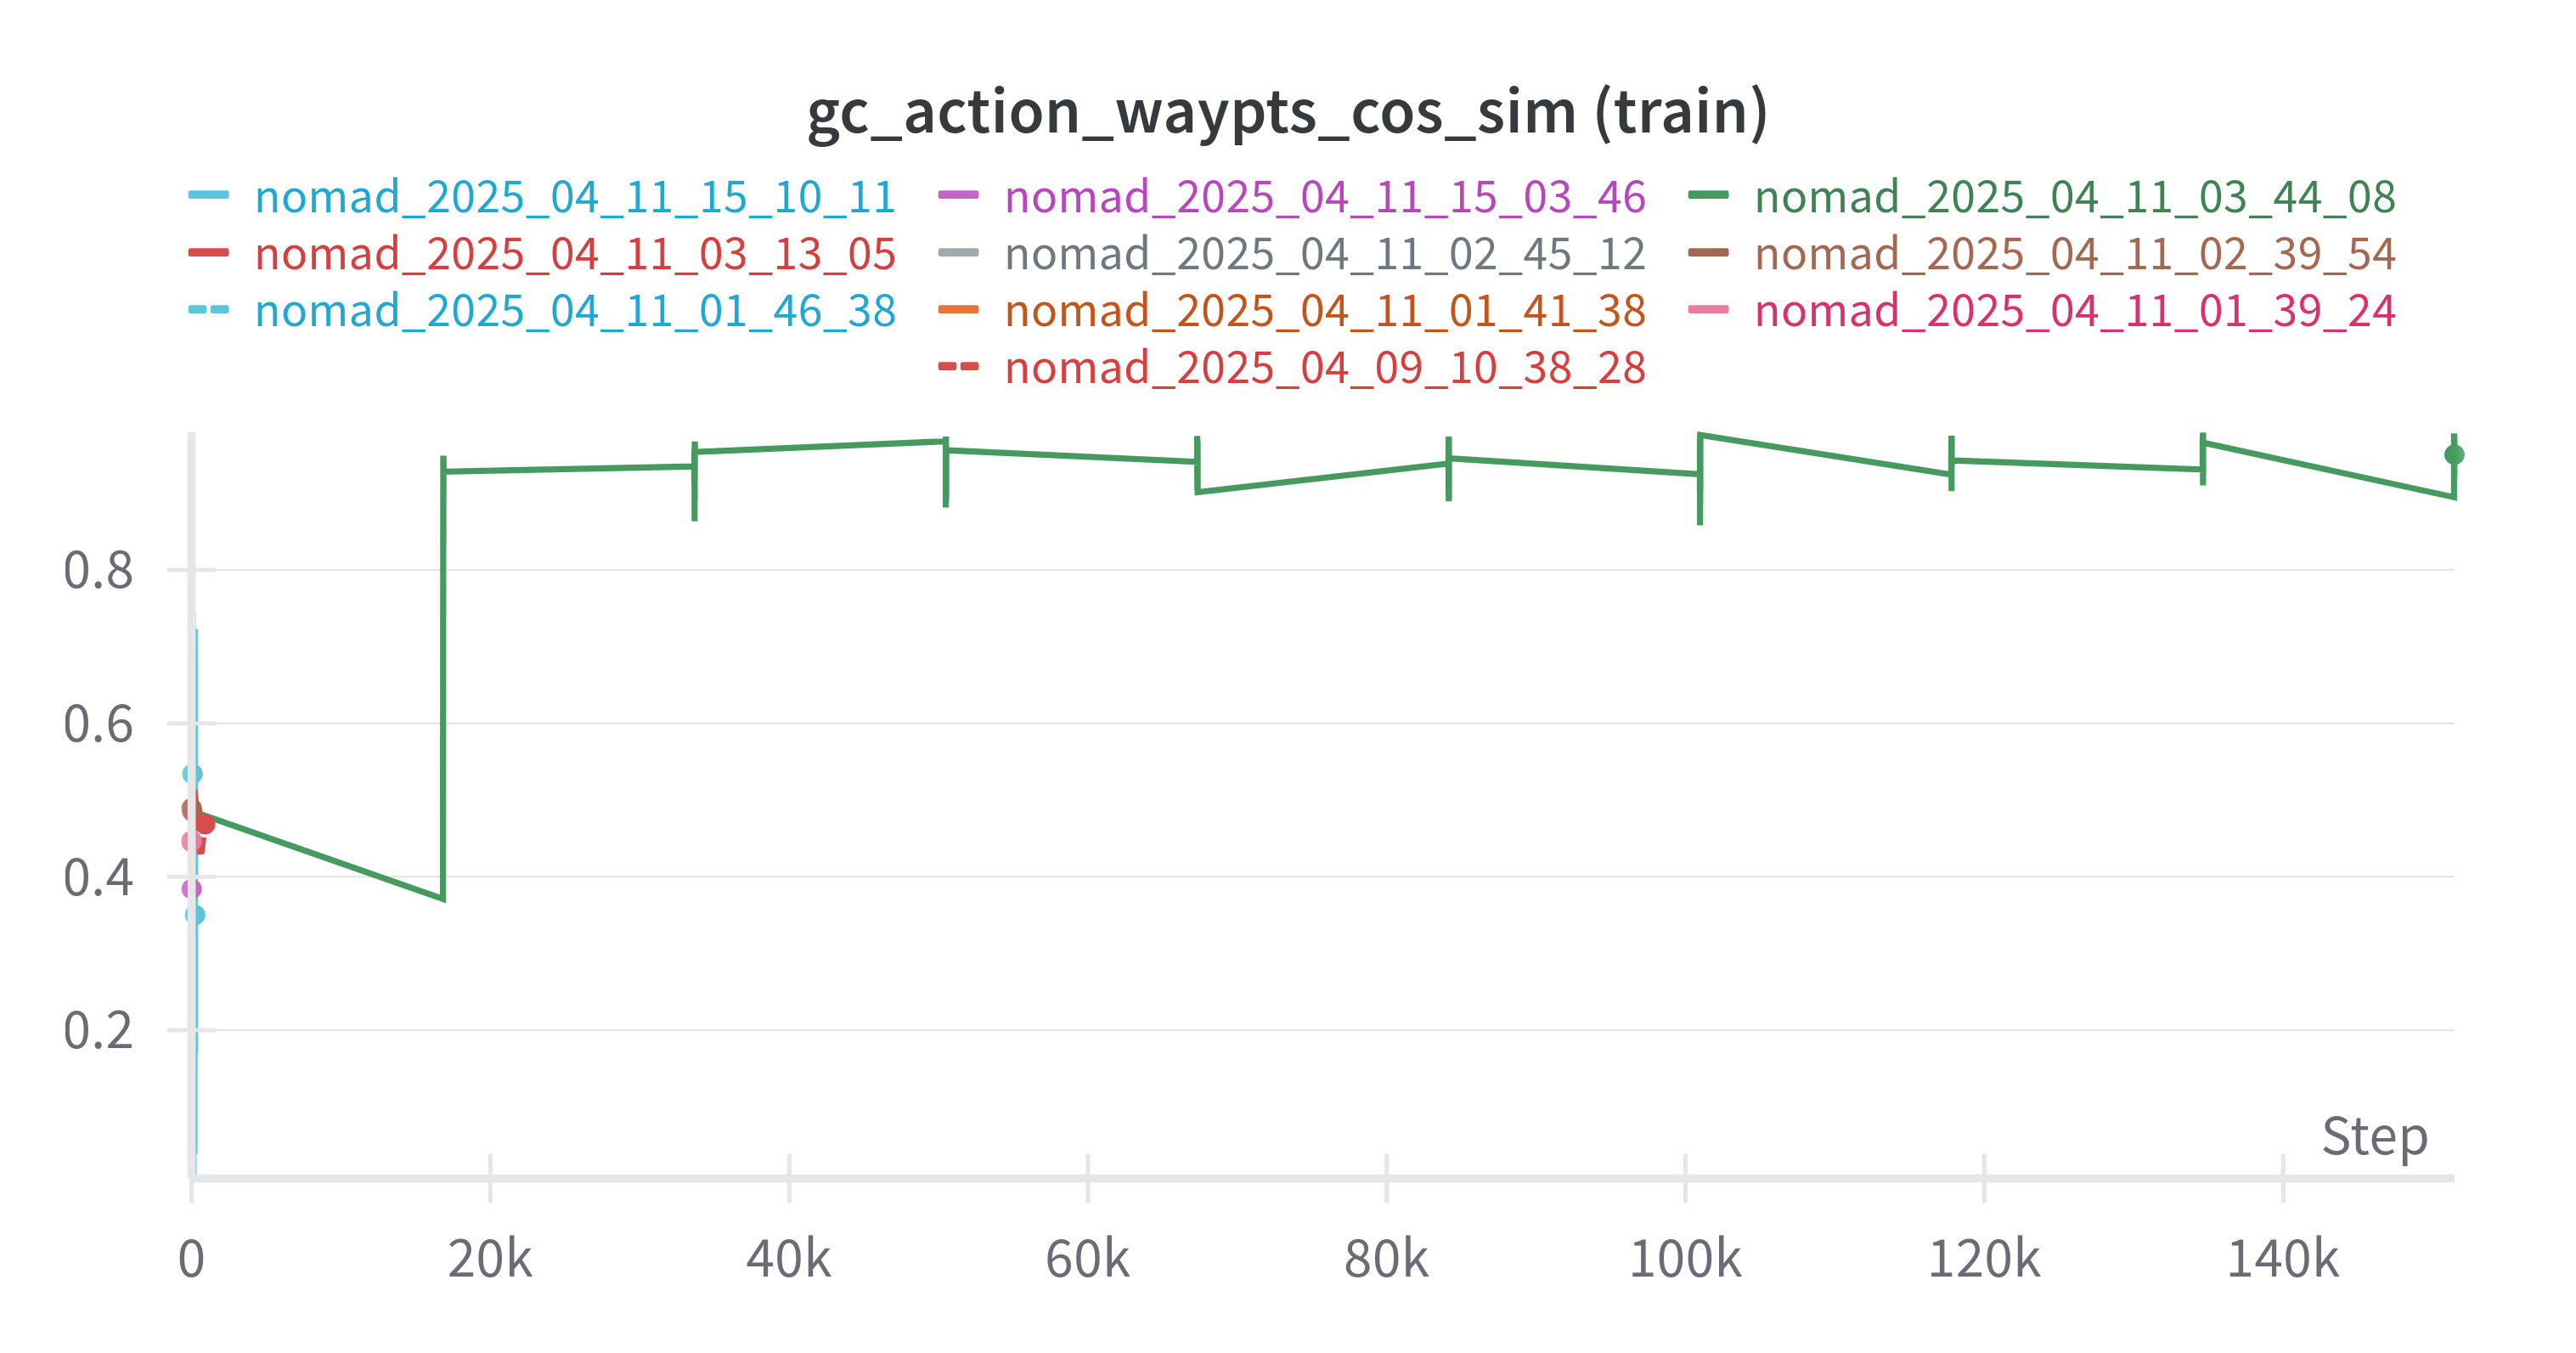
\includegraphics[width=\textwidth]{images/gc_action_sim_nomad.png}

        
            \textbf{Training Set}
        \end{minipage}
        \hfill
        \begin{minipage}{0.48\textwidth}
            \centering
            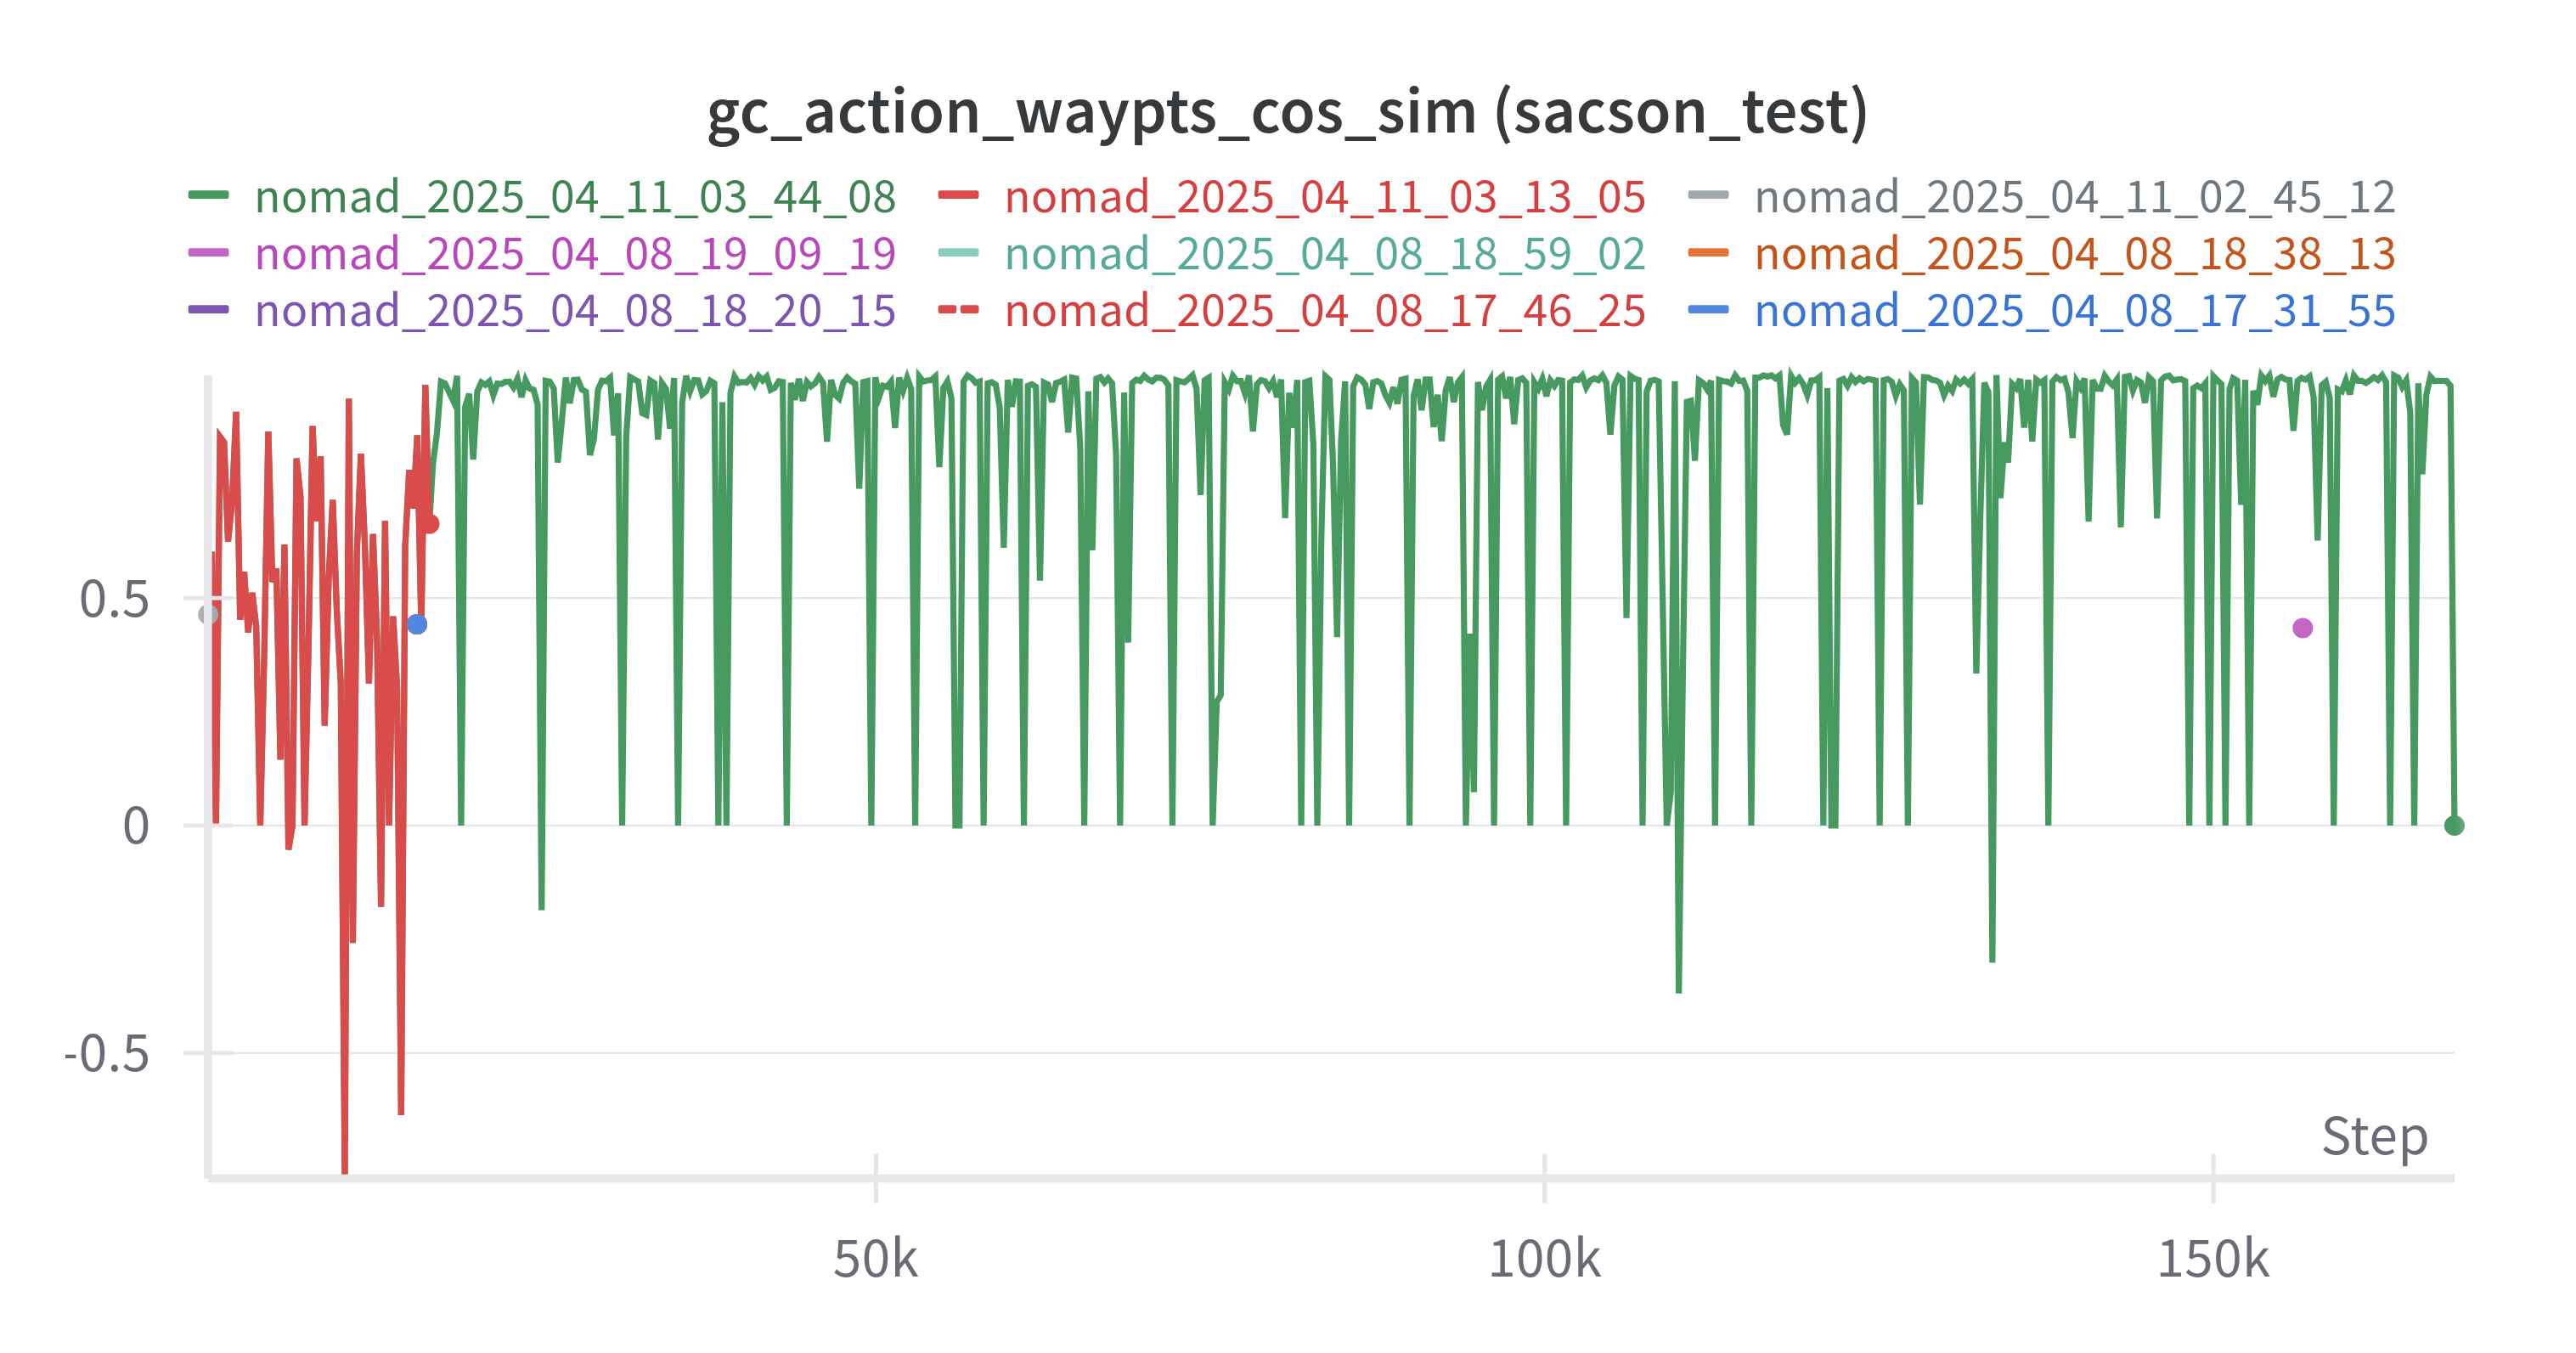
\includegraphics[width=\textwidth]{images/gc_action_cos_sim_test.png}

            \textbf{Validation Set}
        \end{minipage}
        
        \vspace{0.5em}
        \bigskip
        Cosine similarity evaluates directional alignment between predicted and ground-truth action waypoints. 
        Higher values ($\sim1.0$) indicate better trajectory alignment under goal-conditioned settings.
    \end{block}
\end{frame}
\begin{frame}{Experiments and Results: Multi-Action Cosine Similarity}
    \begin{block}{Goal-Conditioned Multi-Action Waypoints Cosine Similarity}
        \begin{minipage}{0.48\textwidth}
            \centering
            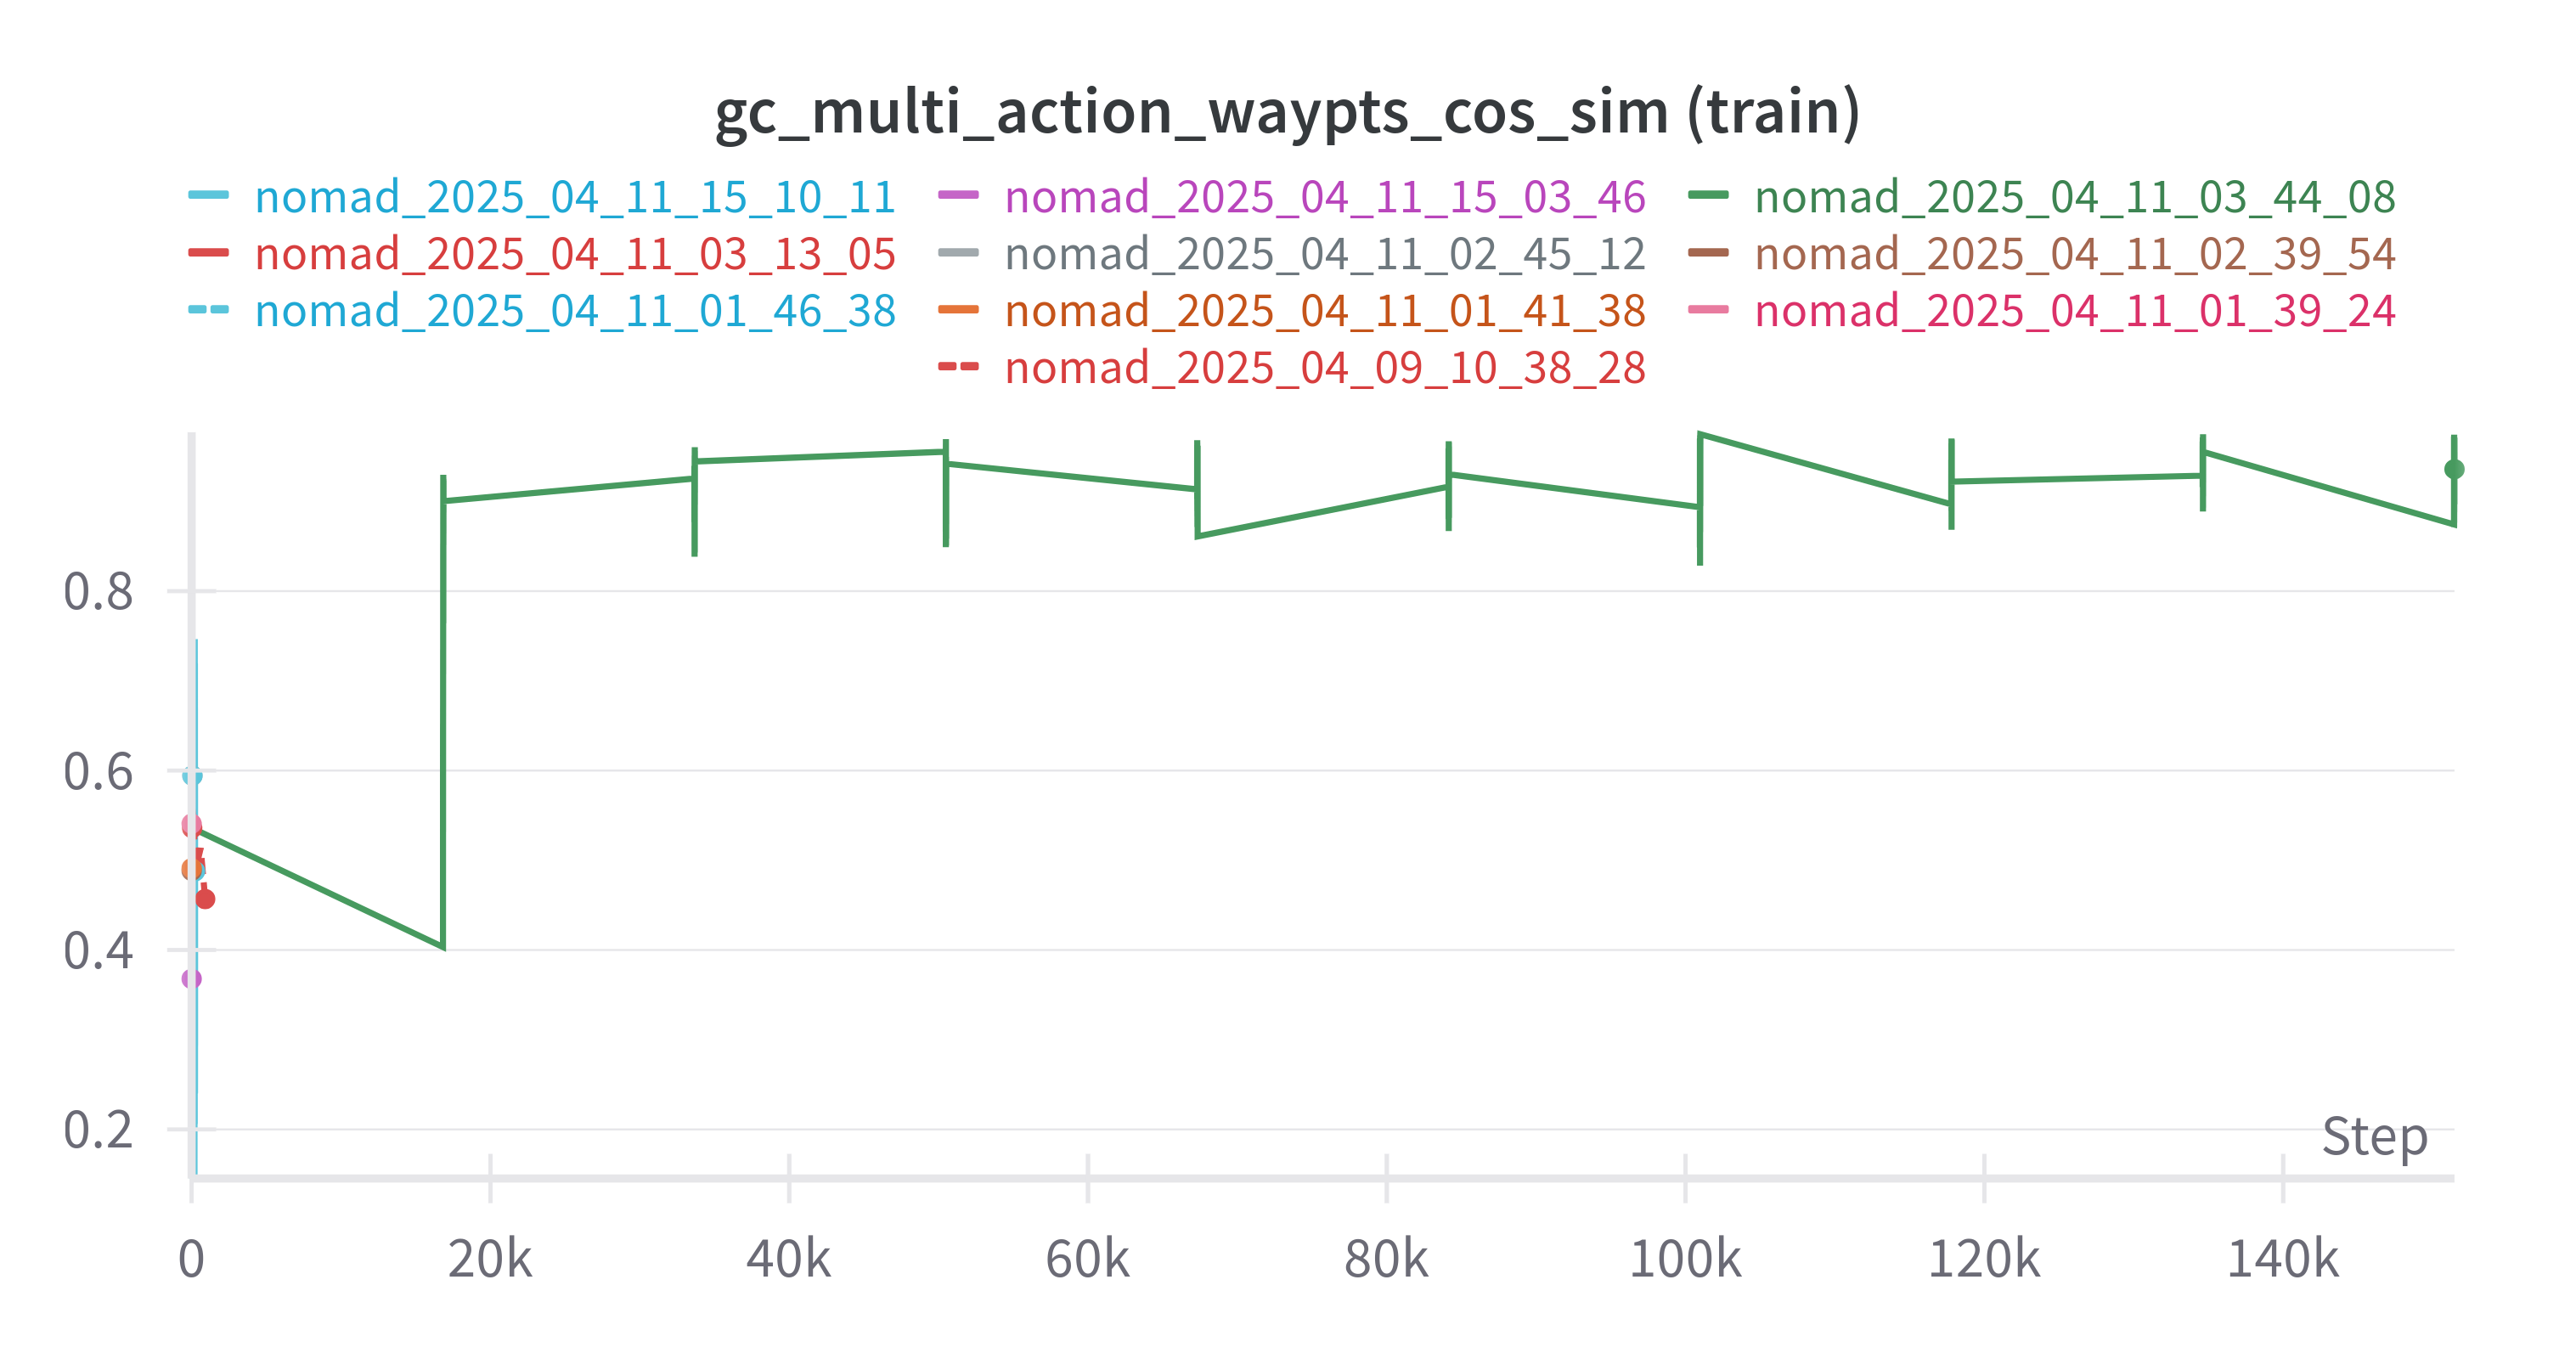
\includegraphics[width=\textwidth]{images/multi_action_sim_train.png}
            
            
            \textbf{Training Set}
        \end{minipage}
        \hfill
        \begin{minipage}{0.48\textwidth}
            \centering
            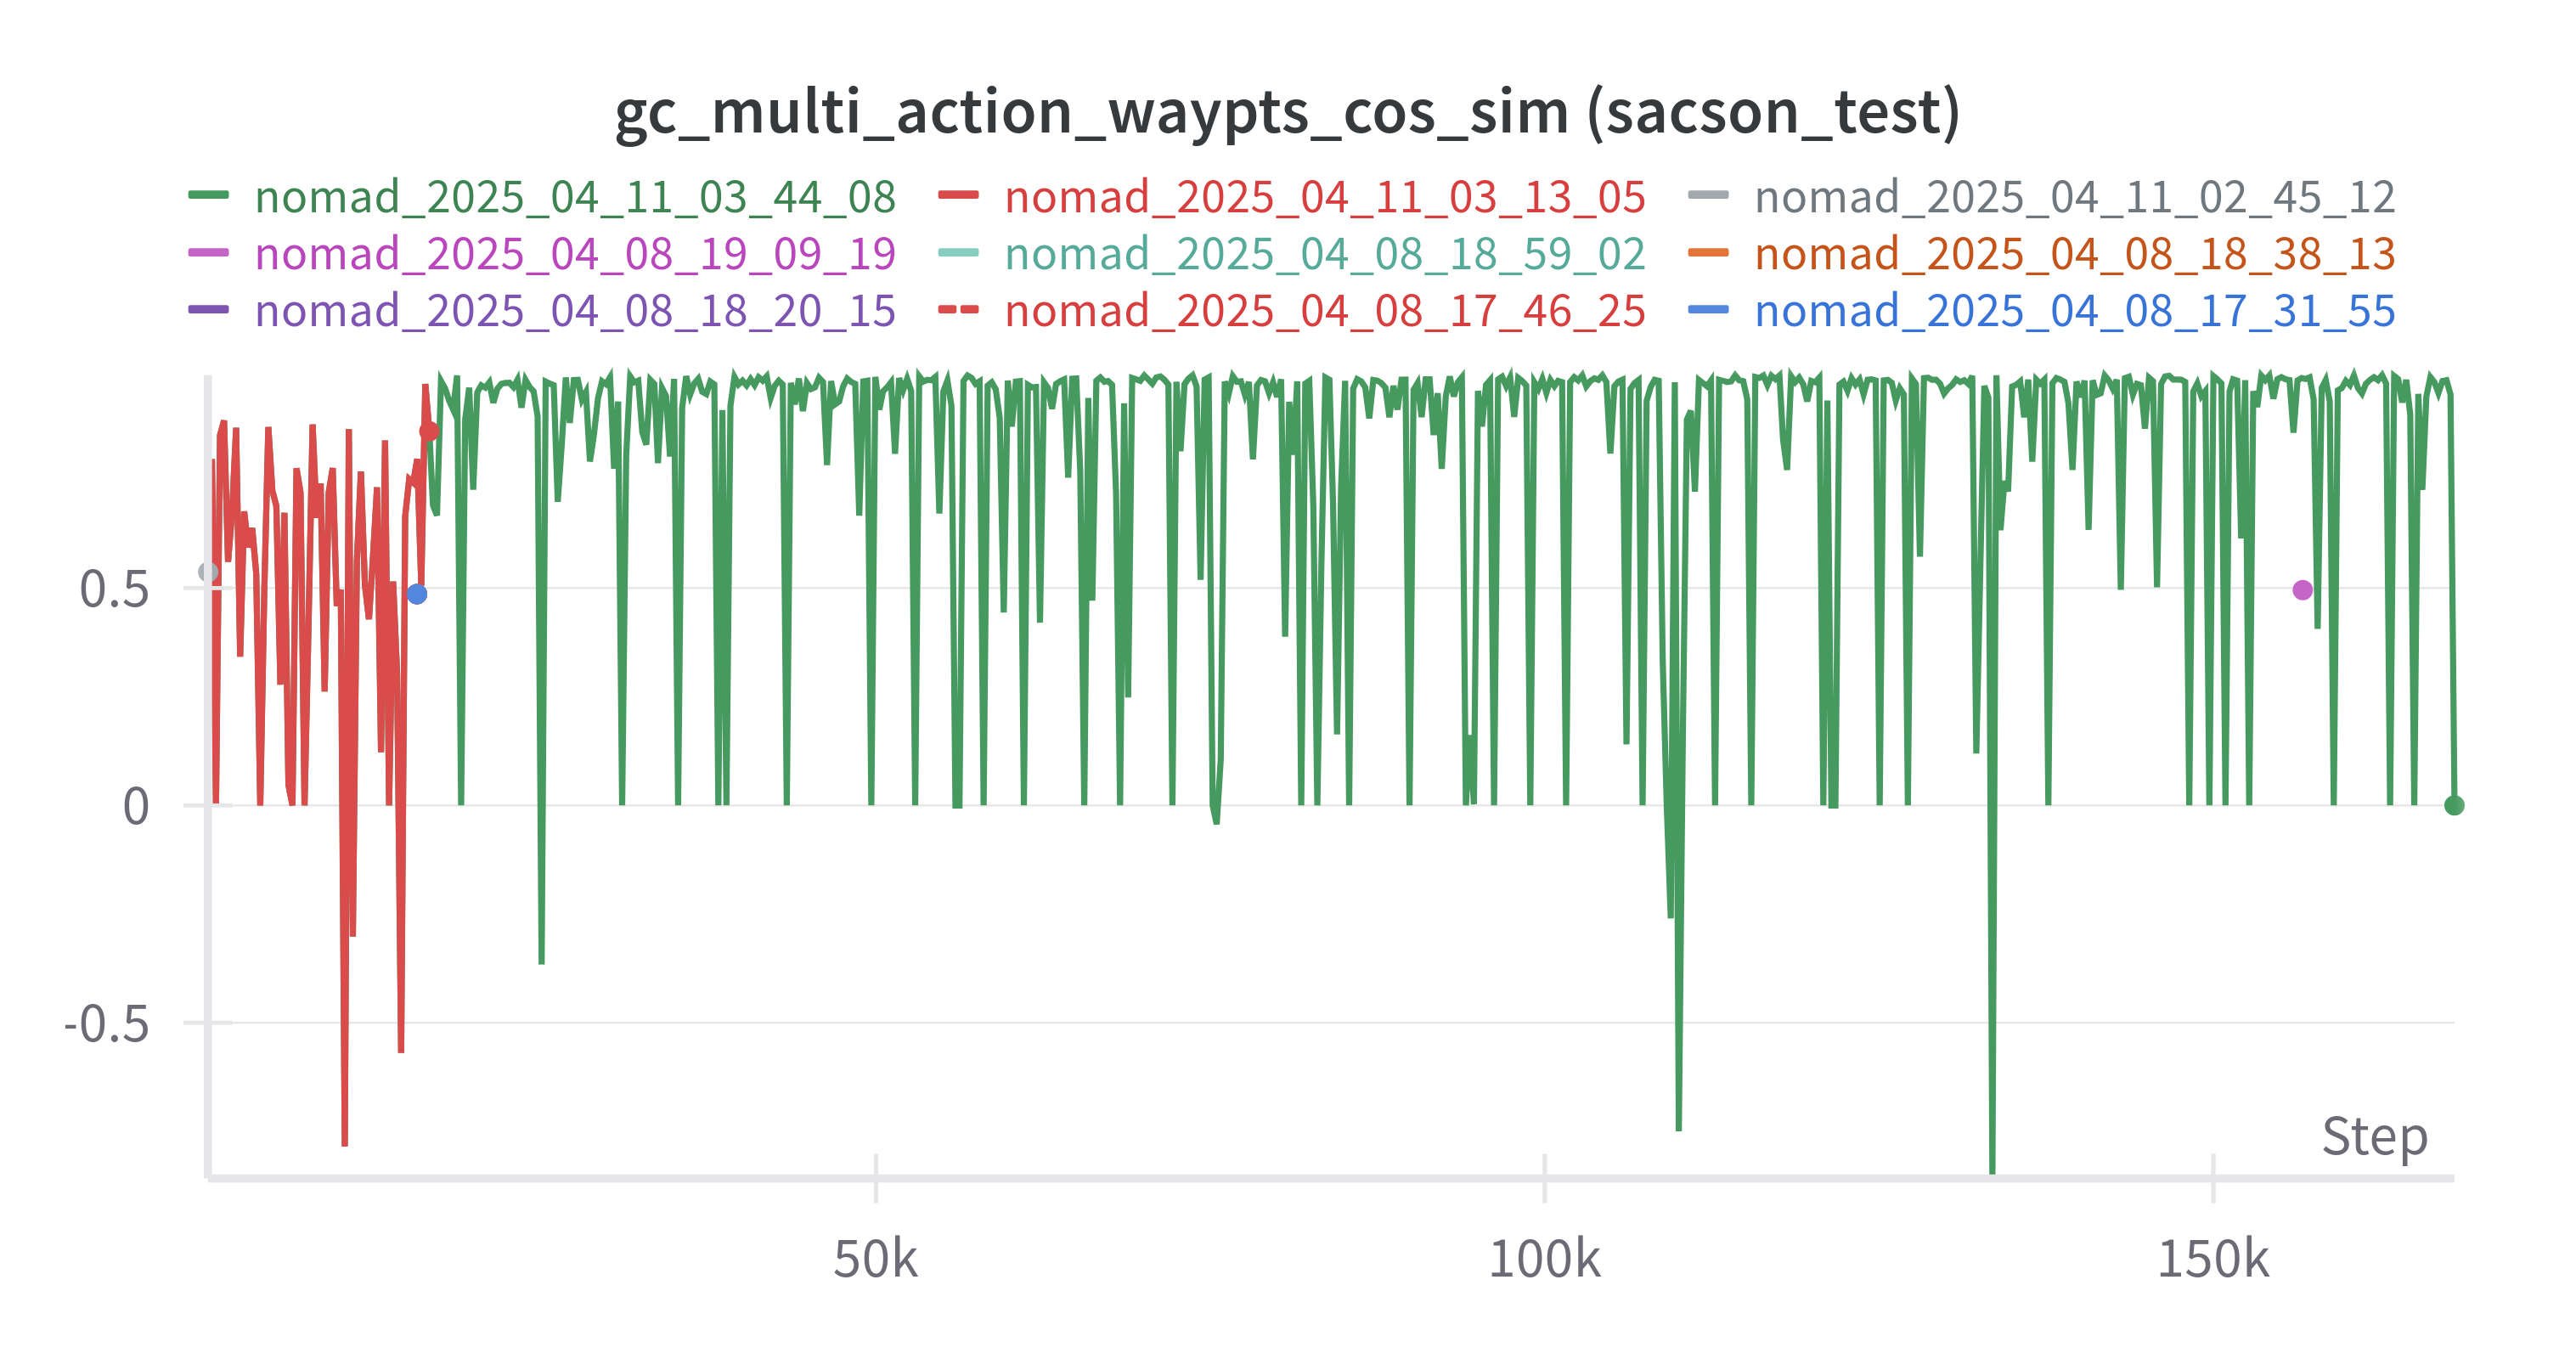
\includegraphics[width=\textwidth]{images/multi_action_sim.png}
        
            
            \textbf{Validation Set}
        \end{minipage}
        
        \vspace{0.5em}
        \bigskip
        Multi-action cosine similarity compares the overall alignment of full predicted trajectory vectors with ground truth, rather than frame-by-frame. This provides a more holistic measure of long-horizon trajectory quality.
    \end{block}
\end{frame}

\begin{frame}{Experiments and Results: UC Multi-Action Cosine Similarity}
    \begin{block}{Unconditioned Multi-Action Waypoints Cosine Similarity}
        \begin{minipage}{0.48\textwidth}
            \centering
            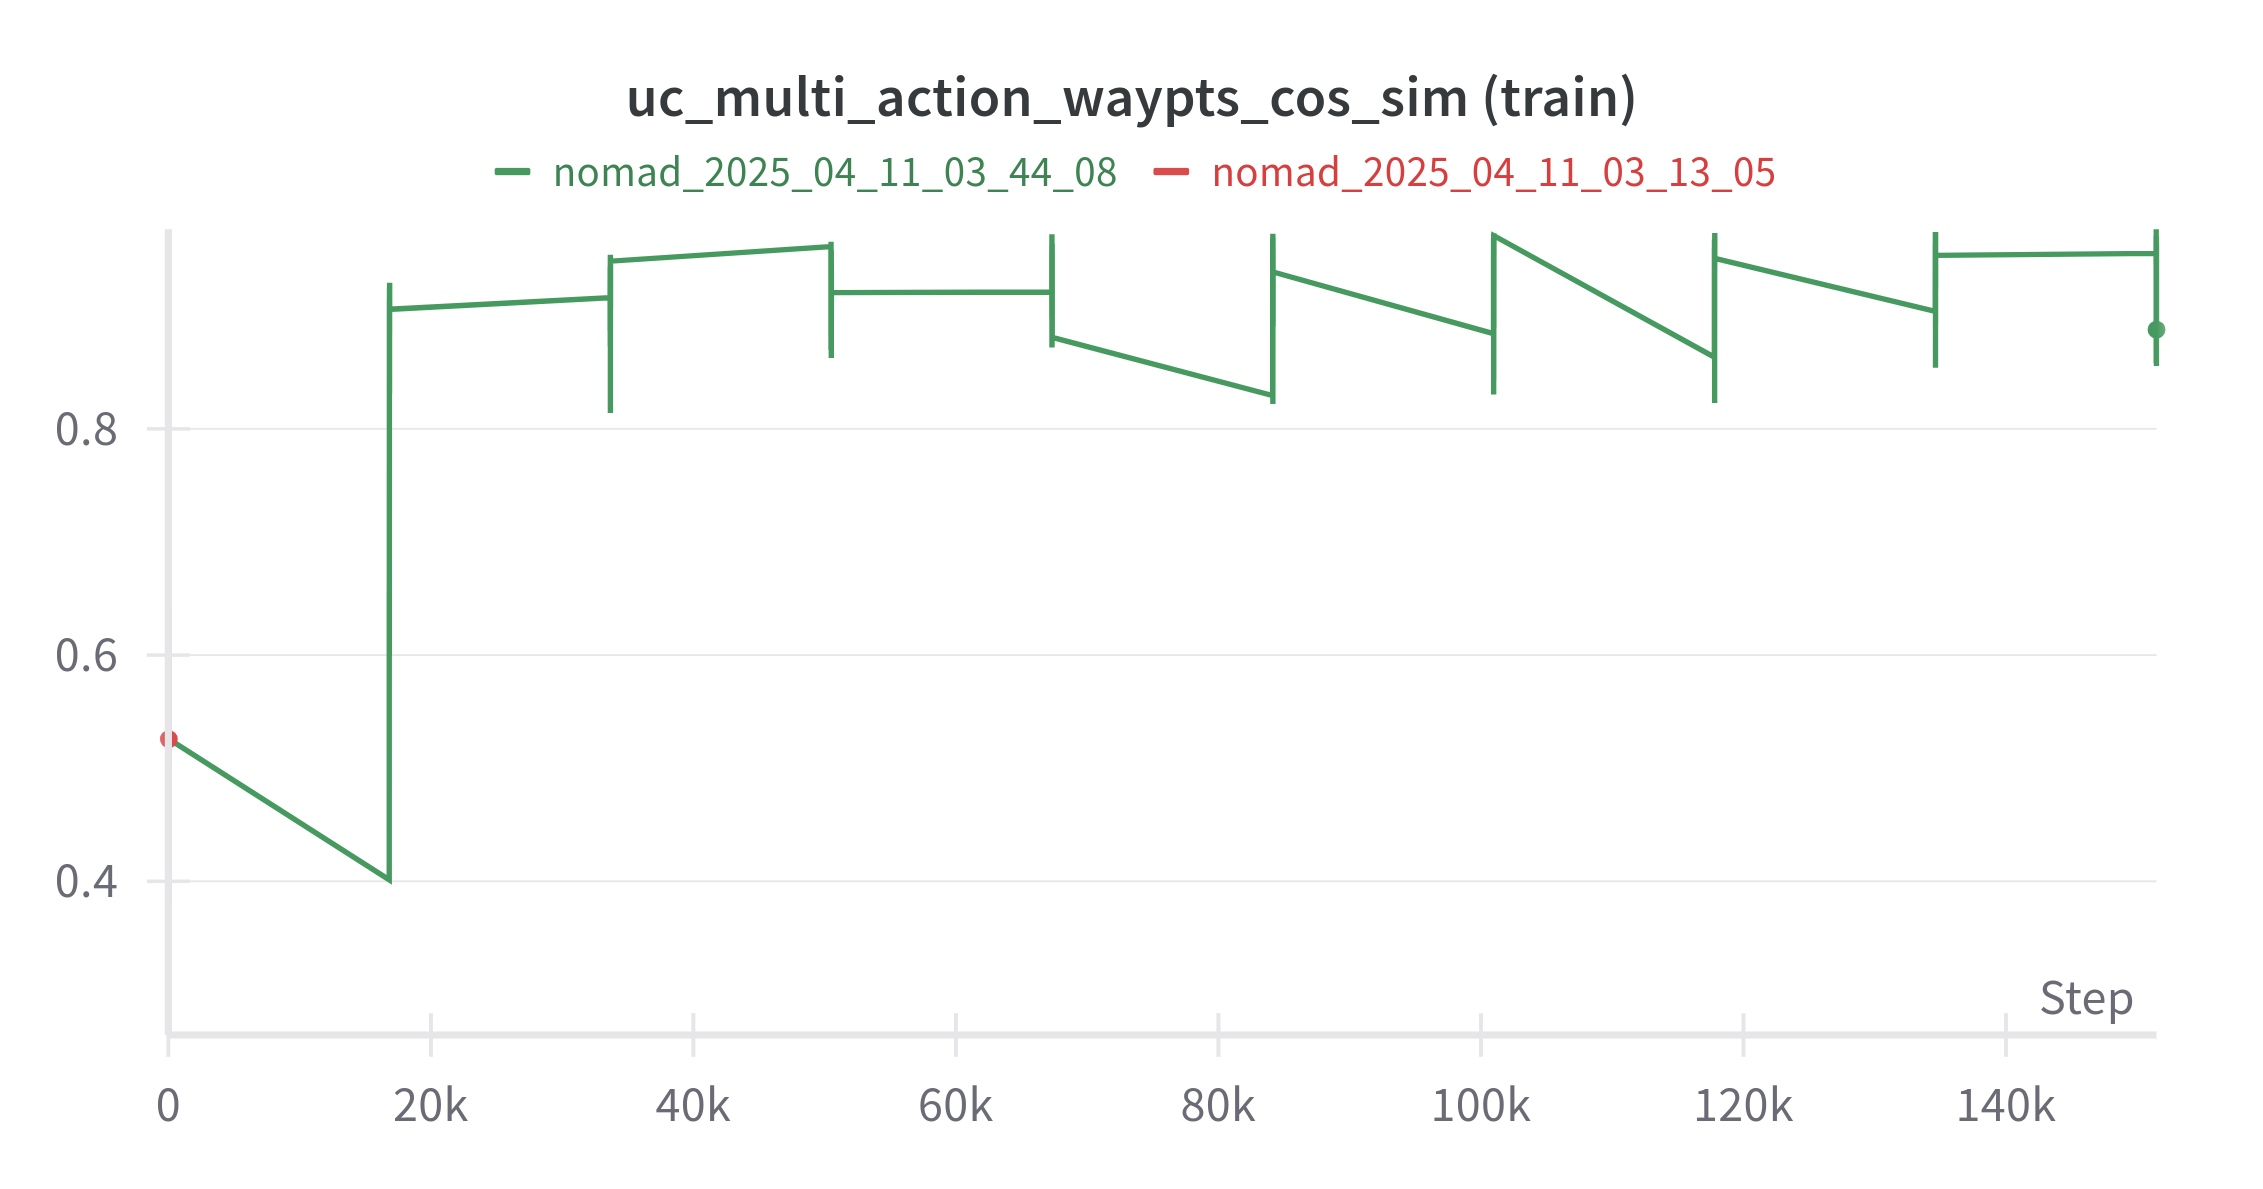
\includegraphics[width=\textwidth]{images/cs_multi_action_cos_train.png}
            
            \textbf{Training Set}
        \end{minipage}
        \hfill
        \begin{minipage}{0.48\textwidth}
            \centering
            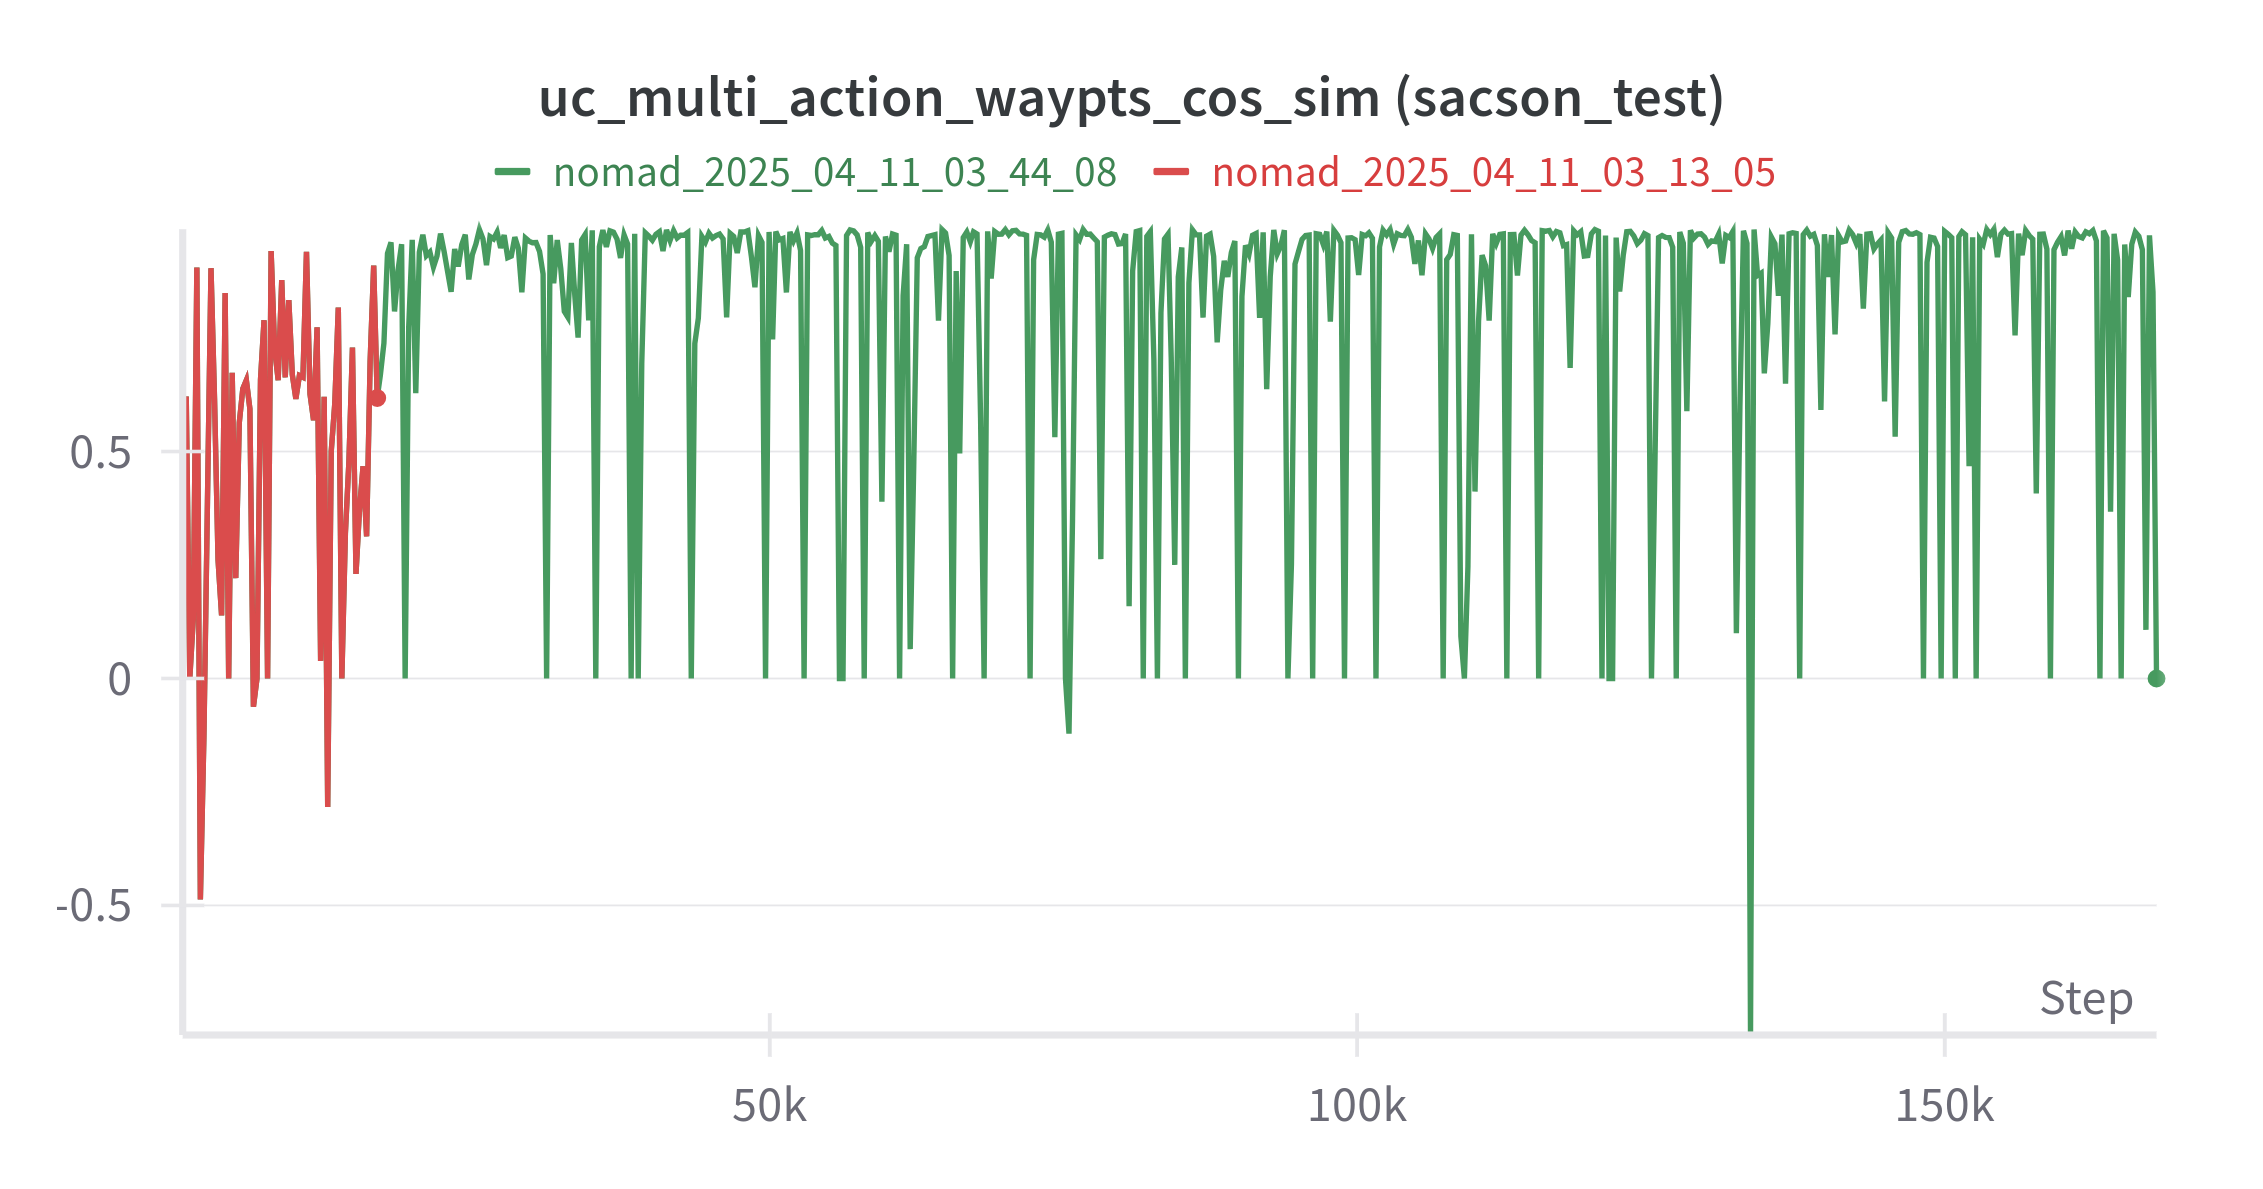
\includegraphics[width=\textwidth]{images/uc_multi_action_sim_test.png}
            
            \textbf{Validation Set}
        \end{minipage}
        
        \vspace{0.5em}
        \bigskip
        Cosine similarity across the full predicted trajectory in unconditioned setting. Higher similarity indicates better alignment with ground-truth behavior.
    \end{block}
\end{frame}
\end{document}
